\chapter{Results and Discussion}\label{cha:discussion}

% \todo{we managed to get a closed loop, to increase speed and to estimate the force. 

% But measurements were shitty because no equipments.
% Model has oscillations because it feedback small forces.
% Friction model improves that from the simulation we made and should be even better when used.
% +Philipe 

% Communication does not reach the aimed refresh rate so force feedback doesn't either.
% Compression should help if it is fast.
% Code should be optimizing by using lower level libraries for communication on linux.
% Safety should be considered more than what we did.
% Consider implementing a real time system like RTAI.

% }

\section{Results}


\todo{The results about communication were already stated in Communication, should they be moved?}

An operator clamps a finger by controlling the Geomagic Touch. As no equipment is available for measuring the force applied by the end-effector, the estimated force is compared with the position error and the current applied to the actuator. The experiment is made for the maximum frequency reached of 638 Hz in \figref{fig:fbkm}, which shows the operator slowly clamping the finger. For comparison, measurements for the original frequency of 100 Hz are displayed in \figref{fig:fbkm_100}, where the operator clamps and releases the finger at a fast pace.


\begin{figure}[H]
  % This file was created by matlab2tikz.
%
%The latest updates can be retrieved from
%  http://www.mathworks.com/matlabcentral/fileexchange/22022-matlab2tikz-matlab2tikz
%where you can also make suggestions and rate matlab2tikz.
%
\definecolor{mycolor1}{rgb}{0.00000,0.44700,0.74100}%
\definecolor{mycolor2}{rgb}{0.85000,0.32500,0.09800}%
%
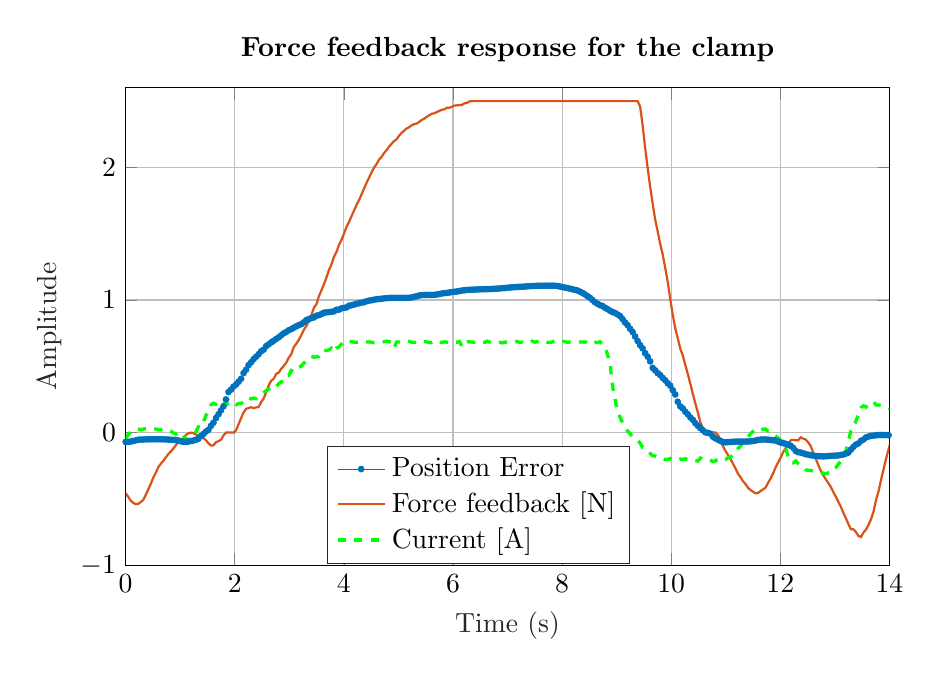
\begin{tikzpicture}

\begin{axis}[%
width=0.8\columnwidth,
height=0.5\columnwidth,
at={(2.512in,1.147in)},
scale only axis,
xmin=0,
xmax=14,
xlabel style={font=\color{white!15!black}},
xlabel={Time (s)},
ymin=-1,
ymax=2.6,
ylabel style={font=\color{white!15!black}},
ylabel={Amplitude},
axis background/.style={fill=white},
title style={font=\bfseries},
title={Force feedback response for the clamp},
xmajorgrids,
ymajorgrids,
legend style={legend cell align=left, align=left, draw=white!15!black, at={(0.66,0.25)}}
]
\addplot [color=mycolor1, draw=none, mark=*, mark size=1,mark options={solid, mycolor1}]
  table[row sep=crcr]{%
0	-0.069839\\
0.046	-0.0691929999999998\\
0.092	-0.0674169999999998\\
0.138	-0.0627580000000001\\
0.184	-0.0585599999999999\\
0.23	-0.053715\\
0.276	-0.052262\\
0.322	-0.0517779999999999\\
0.368	-0.0508089999999999\\
0.414	-0.050325\\
0.46	-0.0500019999999999\\
0.506	-0.0500019999999999\\
0.552	-0.0500019999999999\\
0.598	-0.0500019999999999\\
0.644	-0.050233\\
0.69	-0.0504629999999999\\
0.736	-0.0509360000000001\\
0.782	-0.0523979999999999\\
0.828	-0.0533170000000001\\
0.874	-0.0544640000000001\\
0.92	-0.0558380000000001\\
0.966	-0.059431\\
1.012	-0.0646089999999999\\
1.058	-0.069102\\
1.104	-0.070166\\
1.15	-0.0678619999999999\\
1.196	-0.0632820000000001\\
1.242	-0.0596559999999999\\
1.288	-0.054314\\
1.334	-0.045984\\
1.38	-0.0253700000000001\\
1.426	-0.00976399999999988\\
1.472	0.00805999999999996\\
1.518	0.0212249999999999\\
1.564	0.051482\\
1.61	0.0750869999999999\\
1.656	0.109672\\
1.702	0.138343\\
1.748	0.168177\\
1.794	0.199188\\
1.84	0.250473\\
1.886	0.306211\\
1.932	0.324103\\
1.978	0.347052\\
2.024	0.362787\\
2.07	0.383776\\
2.116	0.406007\\
2.162	0.449559\\
2.208	0.474824\\
2.254	0.508958\\
2.3	0.530804\\
2.346	0.554437\\
2.392	0.572537\\
2.438	0.591942\\
2.484	0.614258\\
2.53	0.625926\\
2.576	0.652916\\
2.622	0.665954\\
2.668	0.680707\\
2.714	0.6931054\\
2.76	0.7064931\\
2.806	0.7187228\\
2.852	0.7341136\\
2.898	0.7492224\\
2.944	0.7593239\\
2.99	0.7720971\\
3.036	0.7809118\\
3.082	0.7910974\\
3.128	0.8020223\\
3.174	0.81066\\
3.22	0.8186307\\
3.266	0.8319814\\
3.312	0.8492741\\
3.358	0.8558223\\
3.404	0.8646376\\
3.45	0.868742\\
3.496	0.8814436\\
3.542	0.8863328\\
3.588	0.8938385\\
3.634	0.9044656\\
3.68	0.9069801\\
3.726	0.9089659\\
3.772	0.9109976\\
3.818	0.9148639\\
3.864	0.9265554\\
3.91	0.9278963\\
3.956	0.9373217\\
4.002	0.940841\\
4.048	0.9445568\\
4.094	0.95726415\\
4.14	0.9604788\\
4.186	0.96597617\\
4.232	0.97119919\\
4.278	0.97641396\\
4.324	0.9801821\\
4.37	0.9838232\\
4.416	0.9907857\\
4.462	0.99572\\
4.508	0.9983443\\
4.554	1.0027004\\
4.6	1.0057562\\
4.646	1.0081051\\
4.692	1.0098843\\
4.738	1.0125273\\
4.784	1.0145615\\
4.83	1.015724\\
4.876	1.0164667\\
4.922	1.0164667\\
4.968	1.0164667\\
5.014	1.0164667\\
5.06	1.0164667\\
5.106	1.0164667\\
5.152	1.0164667\\
5.198	1.017048\\
5.244	1.0196638\\
5.29	1.0246052\\
5.336	1.0286748\\
5.382	1.0344887\\
5.428	1.0368141\\
5.474	1.0379768\\
5.52	1.0385582\\
5.566	1.0385582\\
5.612	1.0385582\\
5.658	1.0391396\\
5.704	1.0420462\\
5.75	1.045534\\
5.796	1.0490214\\
5.842	1.0522178\\
5.888	1.0536705\\
5.934	1.0571568\\
5.98	1.059633\\
6.026	1.062445\\
6.072	1.0644935\\
6.118	1.0679936\\
6.164	1.0718006\\
6.21	1.0739226\\
6.256	1.0760766\\
6.302	1.0773746\\
6.348	1.0781606\\
6.394	1.0786866\\
6.44	1.0796386\\
6.486	1.0806226\\
6.532	1.0811326\\
6.578	1.0815816\\
6.624	1.0821676\\
6.67	1.0826356\\
6.716	1.0836156\\
6.762	1.0849286\\
6.808	1.0862066\\
6.854	1.0874876\\
6.9	1.0889816\\
6.946	1.0904386\\
6.992	1.0921886\\
7.038	1.0943516\\
7.084	1.0958206\\
7.13	1.0971756\\
7.176	1.0983656\\
7.222	1.0995076\\
7.268	1.1005966\\
7.314	1.1015086\\
7.36	1.1031166\\
7.406	1.1045566\\
7.452	1.1057716\\
7.498	1.1059546\\
7.544	1.1072416\\
7.59	1.1076566\\
7.636	1.1080086\\
7.682	1.1083606\\
7.728	1.1083606\\
7.774	1.1082496\\
7.82	1.1082496\\
7.866	1.1078506\\
7.912	1.1055066\\
7.958	1.1023436\\
8.004	1.0977176\\
8.05	1.0940366\\
8.096	1.0909596\\
8.142	1.0861036\\
8.188	1.0816106\\
8.234	1.0766646\\
8.28	1.0723386\\
8.326	1.0637863\\
8.372	1.0543818\\
8.418	1.0428257\\
8.464	1.029448\\
8.51	1.0175659\\
8.556	1.0002029\\
8.602	0.9837055\\
8.648	0.97187785\\
8.694	0.96156563\\
8.74	0.9554396\\
8.786	0.942303\\
8.832	0.9318928\\
8.878	0.9191614\\
8.924	0.9095359\\
8.97	0.9029574\\
9.016	0.8912888\\
9.062	0.879097\\
9.108	0.8563865\\
9.154	0.8307516\\
9.2	0.8113894\\
9.246	0.7837317\\
9.292	0.7592755\\
9.338	0.725409\\
9.384	0.691096\\
9.43	0.659743\\
9.476	0.635184\\
9.522	0.599631\\
9.568	0.572746\\
9.614	0.537474\\
9.66	0.488529\\
9.706	0.470013\\
9.752	0.449131\\
9.798	0.434072\\
9.844	0.412879\\
9.89	0.394881\\
9.936	0.372667\\
9.982	0.354272\\
10.028	0.320757\\
10.074	0.287993\\
10.12	0.232964\\
10.166	0.197741\\
10.212	0.18275\\
10.258	0.156795\\
10.304	0.138484\\
10.35	0.114872\\
10.396	0.097008\\
10.442	0.071595\\
10.488	0.05155\\
10.534	0.034095\\
10.58	0.0179400000000001\\
10.626	0.002305\\
10.672	-0.00167099999999998\\
10.718	-0.00769699999999984\\
10.764	-0.030978\\
10.81	-0.0429710000000001\\
10.856	-0.053148\\
10.902	-0.0618189999999998\\
10.948	-0.0720810000000001\\
10.994	-0.0724389999999999\\
11.04	-0.0717700000000001\\
11.086	-0.0703040000000001\\
11.132	-0.068948\\
11.178	-0.0678830000000001\\
11.224	-0.067339\\
11.27	-0.067339\\
11.316	-0.067339\\
11.362	-0.0671580000000001\\
11.408	-0.0669960000000001\\
11.454	-0.065239\\
11.5	-0.063358\\
11.546	-0.0595410000000001\\
11.592	-0.054964\\
11.638	-0.052603\\
11.684	-0.051604\\
11.73	-0.0518610000000002\\
11.776	-0.053331\\
11.822	-0.0551919999999999\\
11.868	-0.0570810000000002\\
11.914	-0.059763\\
11.96	-0.0673490000000001\\
12.006	-0.075137\\
12.052	-0.0787260000000001\\
12.098	-0.084632\\
12.144	-0.090457\\
12.19	-0.099099\\
12.236	-0.115104\\
12.282	-0.138322\\
12.328	-0.147654\\
12.374	-0.150269\\
12.42	-0.156016\\
12.466	-0.1626\\
12.512	-0.166108\\
12.558	-0.169979\\
12.604	-0.172681\\
12.65	-0.176454\\
12.696	-0.177723\\
12.742	-0.178345\\
12.788	-0.179376\\
12.834	-0.178237\\
12.88	-0.176378\\
12.926	-0.175254\\
12.972	-0.174123\\
13.018	-0.172999\\
13.064	-0.171682\\
13.11	-0.167706\\
13.156	-0.164679\\
13.202	-0.157745\\
13.248	-0.1501\\
13.294	-0.127712\\
13.34	-0.106903\\
13.386	-0.0901689999999999\\
13.432	-0.0812360000000001\\
13.478	-0.0620539999999998\\
13.524	-0.0516510000000001\\
13.57	-0.035822\\
13.616	-0.029779\\
13.662	-0.0236429999999999\\
13.708	-0.0221900000000002\\
13.754	-0.0202520000000002\\
13.8	-0.0181120000000001\\
13.846	-0.018038\\
13.892	-0.018243\\
13.938	-0.0184470000000001\\
13.984	-0.019682\\
14.03	-0.0207010000000001\\
14.076	-0.0221230000000001\\
14.122	-0.023096\\
14.168	-0.023096\\
14.214	-0.023096\\
14.26	-0.0234529999999999\\
14.306	-0.024132\\
14.352	-0.0254239999999999\\
14.398	-0.0299449999999999\\
14.444	-0.033693\\
14.49	-0.0363100000000001\\
14.536	-0.0374399999999999\\
14.582	-0.0393779999999999\\
14.628	-0.039701\\
14.674	-0.0398689999999999\\
14.72	-0.0398770000000002\\
14.766	-0.039682\\
14.812	-0.039682\\
14.858	-0.039682\\
14.904	-0.039682\\
14.95	-0.039682\\
14.996	-0.0391299999999999\\
15.042	-0.0387390000000001\\
15.088	-0.0385439999999999\\
15.134	-0.038152\\
15.18	-0.0377609999999999\\
15.226	-0.0377609999999999\\
15.272	-0.0377609999999999\\
15.318	-0.0377609999999999\\
15.364	-0.0377609999999999\\
15.41	-0.0377609999999999\\
15.456	-0.0375649999999998\\
15.502	-0.0375649999999998\\
15.548	-0.036365\\
15.594	-0.0331220000000001\\
15.64	-0.030756\\
15.686	-0.0297510000000001\\
15.732	-0.02959\\
15.778	-0.028459\\
};
\addlegendentry{Position Error}

\addplot [color=mycolor2, thick]
  table[row sep=crcr]{%
0	-0.457965\\
0.046	-0.482939\\
0.092	-0.512125\\
0.138	-0.528618\\
0.184	-0.539522\\
0.23	-0.537151\\
0.276	-0.524402\\
0.322	-0.507127\\
0.368	-0.470289\\
0.414	-0.428809\\
0.46	-0.387254\\
0.506	-0.339716\\
0.552	-0.303282\\
0.598	-0.26139\\
0.644	-0.235044\\
0.69	-0.212801\\
0.736	-0.186553\\
0.782	-0.161903\\
0.828	-0.14172\\
0.874	-0.120005\\
0.92	-0.094566\\
0.966	-0.0684803\\
1.012	-0.0608241\\
1.058	-0.0433587\\
1.104	-0.0174891\\
1.15	-0.00521286\\
1.196	0.000178016\\
1.242	-0.00297375\\
1.288	-0.0138918\\
1.334	-0.026421\\
1.38	-0.0261145\\
1.426	-0.0405375\\
1.472	-0.0576523\\
1.518	-0.0799315\\
1.564	-0.0976721\\
1.61	-0.0951568\\
1.656	-0.0724242\\
1.702	-0.0633538\\
1.748	-0.0541451\\
1.794	-0.021039\\
1.84	0.000387498\\
1.886	0.00063466\\
1.932	0.000510842\\
1.978	1.40871e-05\\
2.024	0.0176141\\
2.07	0.0641683\\
2.116	0.109299\\
2.162	0.152024\\
2.208	0.179542\\
2.254	0.185892\\
2.3	0.191742\\
2.346	0.185386\\
2.392	0.189675\\
2.438	0.193986\\
2.484	0.230854\\
2.53	0.257935\\
2.576	0.303503\\
2.622	0.357063\\
2.668	0.390772\\
2.714	0.405952\\
2.76	0.443154\\
2.806	0.452801\\
2.852	0.481958\\
2.898	0.503039\\
2.944	0.527297\\
2.99	0.56528\\
3.036	0.591189\\
3.082	0.645425\\
3.128	0.670379\\
3.174	0.699748\\
3.22	0.735109\\
3.266	0.774628\\
3.312	0.805072\\
3.358	0.83938\\
3.404	0.882872\\
3.45	0.942162\\
3.496	0.967106\\
3.542	1.02907\\
3.588	1.07135\\
3.634	1.11914\\
3.68	1.16782\\
3.726	1.22586\\
3.772	1.26648\\
3.818	1.32544\\
3.864	1.36167\\
3.91	1.41453\\
3.956	1.45284\\
4.002	1.50118\\
4.048	1.55186\\
4.094	1.58921\\
4.14	1.63147\\
4.186	1.67488\\
4.232	1.71576\\
4.278	1.75288\\
4.324	1.79633\\
4.37	1.84079\\
4.416	1.88369\\
4.462	1.92324\\
4.508	1.96243\\
4.554	1.99936\\
4.6	2.02567\\
4.646	2.05945\\
4.692	2.08038\\
4.738	2.10928\\
4.784	2.13069\\
4.83	2.15696\\
4.876	2.17937\\
4.922	2.19947\\
4.968	2.21219\\
5.014	2.24018\\
5.06	2.26189\\
5.106	2.27821\\
5.152	2.29389\\
5.198	2.3042\\
5.244	2.31804\\
5.29	2.32692\\
5.336	2.33094\\
5.382	2.34414\\
5.428	2.35817\\
5.474	2.36845\\
5.52	2.38155\\
5.566	2.39363\\
5.612	2.40496\\
5.658	2.40824\\
5.704	2.41806\\
5.75	2.42631\\
5.796	2.4351\\
5.842	2.43808\\
5.888	2.45076\\
5.934	2.45048\\
5.98	2.45716\\
6.026	2.4668\\
6.072	2.46822\\
6.118	2.46973\\
6.164	2.47081\\
6.21	2.48353\\
6.256	2.48696\\
6.302	2.49787\\
6.348	2.5\\
6.394	2.5\\
6.44	2.5\\
6.486	2.5\\
6.532	2.49992\\
6.578	2.5\\
6.624	2.5\\
6.67	2.5\\
6.716	2.5\\
6.762	2.5\\
6.808	2.5\\
6.854	2.5\\
6.9	2.5\\
6.946	2.5\\
6.992	2.5\\
7.038	2.5\\
7.084	2.5\\
7.13	2.5\\
7.176	2.5\\
7.222	2.5\\
7.268	2.5\\
7.314	2.5\\
7.36	2.5\\
7.406	2.5\\
7.452	2.5\\
7.498	2.5\\
7.544	2.5\\
7.59	2.5\\
7.636	2.5\\
7.682	2.5\\
7.728	2.5\\
7.774	2.5\\
7.82	2.5\\
7.866	2.5\\
7.912	2.5\\
7.958	2.5\\
8.004	2.5\\
8.05	2.5\\
8.096	2.5\\
8.142	2.5\\
8.188	2.5\\
8.234	2.5\\
8.28	2.5\\
8.326	2.5\\
8.372	2.5\\
8.418	2.5\\
8.464	2.5\\
8.51	2.5\\
8.556	2.5\\
8.602	2.5\\
8.648	2.5\\
8.694	2.5\\
8.74	2.5\\
8.786	2.5\\
8.832	2.5\\
8.878	2.5\\
8.924	2.5\\
8.97	2.5\\
9.016	2.5\\
9.062	2.5\\
9.108	2.5\\
9.154	2.5\\
9.2	2.5\\
9.246	2.5\\
9.292	2.5\\
9.338	2.5\\
9.384	2.5\\
9.43	2.45972\\
9.476	2.31758\\
9.522	2.14825\\
9.568	1.99722\\
9.614	1.85379\\
9.66	1.72876\\
9.706	1.60717\\
9.752	1.51777\\
9.798	1.42349\\
9.844	1.34486\\
9.89	1.24209\\
9.936	1.13853\\
9.982	1.0087\\
10.028	0.888403\\
10.074	0.786921\\
10.12	0.712798\\
10.166	0.633521\\
10.212	0.58201\\
10.258	0.510575\\
10.304	0.442393\\
10.35	0.369444\\
10.396	0.293081\\
10.442	0.220909\\
10.488	0.152474\\
10.534	0.078849\\
10.58	0.0342911\\
10.626	0.000124028\\
10.672	0.000301921\\
10.718	0.000252726\\
10.764	0.000330059\\
10.81	0.000273753\\
10.856	-0.0174561\\
10.902	-0.0569983\\
10.948	-0.101156\\
10.994	-0.137496\\
11.04	-0.16853\\
11.086	-0.20015\\
11.132	-0.233028\\
11.178	-0.269616\\
11.224	-0.309738\\
11.27	-0.335806\\
11.316	-0.366884\\
11.362	-0.387696\\
11.408	-0.416516\\
11.454	-0.432208\\
11.5	-0.445834\\
11.546	-0.45736\\
11.592	-0.45423\\
11.638	-0.440815\\
11.684	-0.428176\\
11.73	-0.413655\\
11.776	-0.377847\\
11.822	-0.346186\\
11.868	-0.30626\\
11.914	-0.261468\\
11.96	-0.224553\\
12.006	-0.188972\\
12.052	-0.146403\\
12.098	-0.116957\\
12.144	-0.0867584\\
12.19	-0.0573152\\
12.236	-0.0552171\\
12.282	-0.0574377\\
12.328	-0.0575676\\
12.374	-0.0349744\\
12.42	-0.046042\\
12.466	-0.0523814\\
12.512	-0.0740595\\
12.558	-0.101582\\
12.604	-0.151553\\
12.65	-0.197503\\
12.696	-0.243833\\
12.742	-0.288091\\
12.788	-0.321104\\
12.834	-0.352334\\
12.88	-0.379869\\
12.926	-0.410188\\
12.972	-0.449443\\
13.018	-0.483054\\
13.064	-0.523156\\
13.11	-0.558781\\
13.156	-0.606164\\
13.202	-0.644778\\
13.248	-0.689715\\
13.294	-0.72931\\
13.34	-0.729152\\
13.386	-0.749485\\
13.432	-0.779093\\
13.478	-0.786947\\
13.524	-0.753038\\
13.57	-0.730523\\
13.616	-0.695568\\
13.662	-0.65353\\
13.708	-0.595233\\
13.754	-0.50868\\
13.8	-0.441981\\
13.846	-0.355192\\
13.892	-0.275813\\
13.938	-0.196536\\
13.984	-0.125382\\
14.03	-0.0564939\\
14.076	0.000372308\\
14.122	0.000553329\\
14.168	0.000643569\\
14.214	0.000462548\\
14.26	0.00539057\\
14.306	0.0388688\\
14.352	0.0787901\\
14.398	0.106753\\
14.444	0.130374\\
14.49	0.152278\\
14.536	0.170294\\
14.582	0.159808\\
14.628	0.155049\\
14.674	0.143513\\
14.72	0.12149\\
14.766	0.0911616\\
14.812	0.0673271\\
14.858	0.0494943\\
14.904	0.0241393\\
14.95	0.00996927\\
14.996	0.000383604\\
15.042	1.06228e-05\\
15.088	0.000199578\\
15.134	0.00057731\\
15.18	0.000486604\\
15.226	0.000296169\\
15.272	0.000202064\\
15.318	0.000297389\\
15.364	0.000202064\\
15.41	0.000297389\\
15.456	0.000682615\\
15.502	0.000490612\\
15.548	0.000398122\\
15.594	0.00049462\\
15.64	0.000399735\\
15.686	0.000596488\\
15.732	0.000108347\\
15.778	0.000401348\\
};
\addlegendentry{Force feedback [N]}

\addplot [color=green, dashed, very thick]
  table[row sep=crcr]{%
0	-0.0462933\\
0.046	-0.0146618\\
0.092	0.00131416\\
0.138	0.0156918\\
0.184	0.0268745\\
0.23	0.0278339\\
0.276	0.0204849\\
0.322	0.027195\\
0.368	0.0300694\\
0.414	0.0303898\\
0.46	0.026556\\
0.506	0.0262356\\
0.552	0.0275135\\
0.598	0.0217628\\
0.644	0.0211239\\
0.69	0.026556\\
0.736	0.0195255\\
0.782	0.0188866\\
0.828	0.0115376\\
0.874	-0.00220108\\
0.92	-0.00891113\\
0.966	-0.0418205\\
1.012	-0.0236073\\
1.058	-0.0344715\\
1.104	-0.0450153\\
1.15	-0.0504456\\
1.196	-0.0485287\\
1.242	-0.0261631\\
1.288	0.0057869\\
1.334	0.0434895\\
1.38	0.0380573\\
1.426	0.081192\\
1.472	0.129118\\
1.518	0.168417\\
1.564	0.209953\\
1.61	0.222414\\
1.656	0.213787\\
1.702	0.216024\\
1.748	0.229124\\
1.794	0.210911\\
1.84	0.235514\\
1.886	0.200048\\
1.932	0.214746\\
1.978	0.216024\\
2.024	0.209953\\
2.07	0.219858\\
2.116	0.220497\\
2.162	0.229124\\
2.208	0.231041\\
2.254	0.261074\\
2.3	0.255003\\
2.346	0.260756\\
2.392	0.25724\\
2.438	0.278328\\
2.484	0.286955\\
2.53	0.301332\\
2.576	0.316988\\
2.622	0.329769\\
2.668	0.333603\\
2.714	0.356928\\
2.76	0.346703\\
2.806	0.368429\\
2.852	0.383766\\
2.898	0.388559\\
2.944	0.428497\\
2.99	0.431053\\
3.036	0.468117\\
3.082	0.458851\\
3.128	0.487926\\
3.174	0.492718\\
3.22	0.502623\\
3.266	0.524349\\
3.312	0.540007\\
3.358	0.557259\\
3.404	0.57675\\
3.45	0.56908\\
3.496	0.571957\\
3.542	0.575151\\
3.588	0.605825\\
3.634	0.625315\\
3.68	0.618925\\
3.726	0.624355\\
3.772	0.636816\\
3.818	0.607422\\
3.864	0.637775\\
3.91	0.646082\\
3.956	0.668768\\
4.002	0.687618\\
4.048	0.682827\\
4.094	0.686979\\
4.14	0.686022\\
4.186	0.682186\\
4.232	0.681547\\
4.278	0.683466\\
4.324	0.682507\\
4.37	0.681868\\
4.416	0.682827\\
4.462	0.684423\\
4.508	0.681547\\
4.554	0.677713\\
4.6	0.681868\\
4.646	0.680908\\
4.692	0.685062\\
4.738	0.685383\\
4.784	0.690174\\
4.83	0.685383\\
4.876	0.682507\\
4.922	0.640331\\
4.968	0.684105\\
5.014	0.683466\\
5.06	0.681229\\
5.106	0.687939\\
5.152	0.685701\\
5.198	0.688257\\
5.244	0.681229\\
5.29	0.679312\\
5.336	0.684744\\
5.382	0.688896\\
5.428	0.682827\\
5.474	0.687618\\
5.52	0.684105\\
5.566	0.67963\\
5.612	0.678034\\
5.658	0.687939\\
5.704	0.682507\\
5.75	0.686661\\
5.796	0.678991\\
5.842	0.684744\\
5.888	0.681868\\
5.934	0.685701\\
5.98	0.687939\\
6.026	0.681868\\
6.072	0.681868\\
6.118	0.687618\\
6.164	0.648638\\
6.21	0.681229\\
6.256	0.685701\\
6.302	0.684423\\
6.348	0.683784\\
6.394	0.681229\\
6.44	0.688578\\
6.486	0.681868\\
6.532	0.682186\\
6.578	0.68059\\
6.624	0.689856\\
6.67	0.683466\\
6.716	0.689856\\
6.762	0.682827\\
6.808	0.681229\\
6.854	0.680908\\
6.9	0.676756\\
6.946	0.682507\\
6.992	0.682827\\
7.038	0.680908\\
7.084	0.681229\\
7.13	0.68059\\
7.176	0.687939\\
7.222	0.678352\\
7.268	0.682827\\
7.314	0.6742\\
7.36	0.682827\\
7.406	0.682827\\
7.452	0.690174\\
7.498	0.681547\\
7.544	0.686979\\
7.59	0.685383\\
7.636	0.684744\\
7.682	0.692091\\
7.728	0.682186\\
7.774	0.678673\\
7.82	0.684744\\
7.866	0.692091\\
7.912	0.685383\\
7.958	0.682827\\
8.004	0.689535\\
8.05	0.685383\\
8.096	0.681547\\
8.142	0.683146\\
8.188	0.679951\\
8.234	0.682186\\
8.28	0.683784\\
8.326	0.683466\\
8.372	0.683784\\
8.418	0.681547\\
8.464	0.69273\\
8.51	0.680269\\
8.556	0.678034\\
8.602	0.680908\\
8.648	0.67963\\
8.694	0.685701\\
8.74	0.667809\\
8.786	0.65439\\
8.832	0.587612\\
8.878	0.522753\\
8.924	0.353092\\
8.97	0.255323\\
9.016	0.151484\\
9.062	0.117296\\
9.108	0.0735226\\
9.154	0.0380573\\
9.2	0.0124969\\
9.246	-0.00699234\\
9.292	-0.0335121\\
9.338	-0.043417\\
9.384	-0.0552387\\
9.43	-0.0792027\\
9.476	-0.110834\\
9.522	-0.115625\\
9.568	-0.141827\\
9.614	-0.156843\\
9.66	-0.174736\\
9.706	-0.176014\\
9.752	-0.183681\\
9.798	-0.182404\\
9.844	-0.197102\\
9.89	-0.203171\\
9.936	-0.201254\\
9.982	-0.195503\\
10.028	-0.207645\\
10.074	-0.211479\\
10.12	-0.208923\\
10.166	-0.199337\\
10.212	-0.202213\\
10.258	-0.196781\\
10.304	-0.204449\\
10.35	-0.202852\\
10.396	-0.202213\\
10.442	-0.209881\\
10.488	-0.214354\\
10.534	-0.191988\\
10.58	-0.20381\\
10.626	-0.202532\\
10.672	-0.203171\\
10.718	-0.208284\\
10.764	-0.21755\\
10.81	-0.212437\\
10.856	-0.201574\\
10.902	-0.212118\\
10.948	-0.202532\\
10.994	-0.201893\\
11.04	-0.190392\\
11.086	-0.184641\\
11.132	-0.171221\\
11.178	-0.150454\\
11.224	-0.119141\\
11.27	-0.100929\\
11.316	-0.0760078\\
11.362	-0.0552387\\
11.408	-0.0299988\\
11.454	-0.0085907\\
11.5	0.00866318\\
11.546	0.0224018\\
11.592	0.0313473\\
11.638	0.019846\\
11.684	0.0259171\\
11.73	0.027195\\
11.776	0.011219\\
11.822	0.00866318\\
11.868	-0.0140228\\
11.914	-0.0271225\\
11.96	-0.0399017\\
12.006	-0.058115\\
12.052	-0.0986919\\
12.098	-0.1201\\
12.144	-0.177292\\
12.19	-0.223619\\
12.236	-0.228094\\
12.282	-0.213715\\
12.328	-0.234484\\
12.374	-0.251417\\
12.42	-0.258127\\
12.466	-0.280811\\
12.512	-0.283369\\
12.558	-0.285925\\
12.604	-0.290716\\
12.65	-0.299664\\
12.696	-0.305414\\
12.742	-0.307331\\
12.788	-0.305414\\
12.834	-0.309568\\
12.88	-0.303177\\
12.926	-0.30126\\
12.972	-0.274742\\
13.018	-0.263878\\
13.064	-0.237679\\
13.11	-0.216272\\
13.156	-0.174736\\
13.202	-0.137352\\
13.248	-0.0641861\\
13.294	0.0150528\\
13.34	0.0339031\\
13.386	0.0882206\\
13.432	0.139662\\
13.478	0.188227\\
13.524	0.202286\\
13.57	0.193338\\
13.616	0.21826\\
13.662	0.226248\\
13.708	0.234556\\
13.754	0.208355\\
13.8	0.208994\\
13.846	0.203243\\
13.892	0.196533\\
13.938	0.189505\\
13.984	0.18631\\
14.03	0.17321\\
14.076	0.157873\\
14.122	0.146051\\
14.168	0.111225\\
14.214	0.0952492\\
14.26	0.0613823\\
14.306	0.0450859\\
14.352	0.0188866\\
14.398	-0.00571442\\
14.444	-0.0213718\\
14.49	-0.0296783\\
14.536	-0.0402222\\
14.582	-0.0309563\\
14.628	-0.0306377\\
14.674	-0.036068\\
14.72	-0.0379848\\
14.766	-0.0357494\\
14.812	-0.0312767\\
14.858	-0.0383053\\
14.904	-0.0303173\\
14.95	-0.0306377\\
14.996	-0.0296783\\
15.042	-0.0216904\\
15.088	-0.0216904\\
15.134	-0.0137024\\
15.18	0.000675201\\
15.226	-0.00251961\\
15.272	0.0124969\\
15.318	0.0131359\\
15.364	0.0211239\\
15.41	0.0255966\\
15.456	0.0287914\\
15.502	0.0310287\\
15.548	0.0326252\\
15.594	0.0262356\\
15.64	0.0294304\\
15.686	0.0422115\\
15.732	0.0479622\\
15.778	0.0447674\\
};
\addlegendentry{Current [A]}

\end{axis}
\end{tikzpicture}%
  \caption{Clamping a finger using a refresh rate of 638 Hz for the communication}
  \label{fig:fbkm}
\end{figure}

\begin{figure}[H]
  % This file was created by matlab2tikz.
%
%The latest updates can be retrieved from
%  http://www.mathworks.com/matlabcentral/fileexchange/22022-matlab2tikz-matlab2tikz
%where you can also make suggestions and rate matlab2tikz.
%
\definecolor{mycolor1}{rgb}{0.00000,0.44700,0.74100}%
\definecolor{mycolor2}{rgb}{0.85000,0.32500,0.09800}%
%
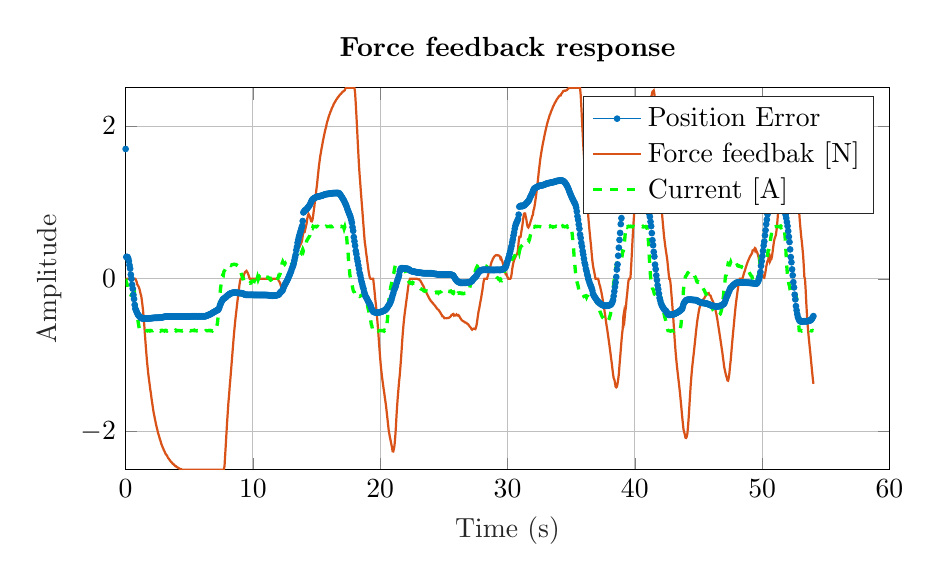
\begin{tikzpicture}

\begin{axis}[%
width=0.8\columnwidth,
height=0.4\columnwidth,
at={(2.512in,1.147in)},
scale only axis,
xmin=0,
xmax=60,
xlabel style={font=\color{white!15!black}},
xlabel={Time (s)},
ymin=-2.5,
ymax=2.5,
ylabel style={font=\color{white!15!black}},
ylabel={Amplitude},
axis background/.style={fill=white},
title style={font=\bfseries},
title={Force feedback response},
xmajorgrids,
ymajorgrids,
legend style={legend cell align=left, align=left, draw=white!15!black}
]
\addplot [color=mycolor1, draw=none, mark=*, mark size=1,  mark options={solid, mycolor1}]
  table[row sep=crcr]{%
0	1.7\\
0.0507779121398926	0.28547\\
0.101555824279785	0.285632\\
0.152333736419678	0.28547\\
0.20311164855957	0.265286\\
0.253889560699463	0.232825\\
0.304667472839355	0.179853\\
0.355445384979248	0.133506\\
0.406223297119141	0.05487\\
0.457001209259033	0.000454000000000065\\
0.507779121398926	-0.078344\\
0.558557033538818	-0.129526\\
0.609334945678711	-0.210262\\
0.660112857818604	-0.264355\\
0.710890769958496	-0.340569\\
0.761668682098389	-0.389818\\
0.812446594238281	-0.409841\\
0.863224506378174	-0.43277\\
0.914002418518066	-0.44924\\
0.964780330657959	-0.468778\\
1.01555824279785	-0.479116\\
1.06633615493774	-0.490258\\
1.11711406707764	-0.496878\\
1.16789197921753	-0.500754\\
1.21866989135742	-0.51351\\
1.26944780349731	-0.517708\\
1.32022571563721	-0.518036\\
1.3710036277771	-0.518367\\
1.42178153991699	-0.518698\\
1.47255945205688	-0.519029\\
1.52333736419678	-0.519194\\
1.57411527633667	-0.519194\\
1.62489318847656	-0.519194\\
1.67567110061646	-0.518993\\
1.72644901275635	-0.518993\\
1.77722692489624	-0.518728\\
1.82800483703613	-0.518066\\
1.87878274917603	-0.517467\\
1.92956066131592	-0.516803\\
1.98033857345581	-0.516\\
2.0311164855957	-0.515297\\
2.0818943977356	-0.513756\\
2.13267230987549	-0.513084\\
2.18345022201538	-0.512242\\
2.23422813415527	-0.511398\\
2.28500604629517	-0.510721\\
2.33578395843506	-0.510382\\
2.38656187057495	-0.510043\\
2.43733978271484	-0.509363\\
2.48811769485474	-0.509363\\
2.53889560699463	-0.509363\\
2.58967351913452	-0.509193\\
2.64045143127441	-0.508511\\
2.69122934341431	-0.50834\\
2.7420072555542	-0.507725\\
2.79278516769409	-0.50704\\
2.84356307983398	-0.505462\\
2.89434099197388	-0.503364\\
2.94511890411377	-0.501222\\
2.99589681625366	-0.498786\\
3.04667472839355	-0.497562\\
3.09745264053345	-0.495382\\
3.14823055267334	-0.494077\\
3.19900846481323	-0.493901\\
3.24978637695312	-0.493725\\
3.30056428909302	-0.493618\\
3.35134220123291	-0.493618\\
3.4021201133728	-0.493618\\
3.4528980255127	-0.493618\\
3.50367593765259	-0.493618\\
3.55445384979248	-0.493511\\
3.60523176193237	-0.493243\\
3.65600967407227	-0.493243\\
3.70678758621216	-0.493243\\
3.75756549835205	-0.493243\\
3.80834341049194	-0.493243\\
3.85912132263184	-0.493243\\
3.90989923477173	-0.493243\\
3.96067714691162	-0.493135\\
4.01145505905151	-0.493027\\
4.06223297119141	-0.492919\\
4.1130108833313	-0.492919\\
4.16378879547119	-0.492919\\
4.21456670761108	-0.492919\\
4.26534461975098	-0.492919\\
4.31612253189087	-0.492919\\
4.36690044403076	-0.492919\\
4.41767835617065	-0.492919\\
4.46845626831055	-0.492811\\
4.51923418045044	-0.492811\\
4.57001209259033	-0.492811\\
4.62079000473022	-0.492811\\
4.67156791687012	-0.492811\\
4.72234582901001	-0.492811\\
4.7731237411499	-0.492811\\
4.82390165328979	-0.492811\\
4.87467956542969	-0.492703\\
4.92545747756958	-0.492703\\
4.97623538970947	-0.492703\\
5.02701330184937	-0.492487\\
5.07779121398926	-0.492161\\
5.12856912612915	-0.491288\\
5.17934703826904	-0.491068\\
5.23012495040894	-0.490959\\
5.28090286254883	-0.490959\\
5.33168077468872	-0.490959\\
5.38245868682861	-0.490959\\
5.43323659896851	-0.490849\\
5.4840145111084	-0.490849\\
5.53479242324829	-0.491025\\
5.58557033538818	-0.491025\\
5.63634824752808	-0.491025\\
5.68712615966797	-0.491025\\
5.73790407180786	-0.491025\\
5.78868198394775	-0.491025\\
5.83945989608765	-0.491025\\
5.89023780822754	-0.491025\\
5.94101572036743	-0.491025\\
5.99179363250732	-0.491025\\
6.04257154464722	-0.491025\\
6.09334945678711	-0.491025\\
6.144127368927	-0.491025\\
6.19490528106689	-0.491025\\
6.24568319320679	-0.491025\\
6.29646110534668	-0.488728\\
6.34723901748657	-0.484861\\
6.39801692962646	-0.481097\\
6.44879484176636	-0.47744\\
6.49957275390625	-0.473755\\
6.55035066604614	-0.469556\\
6.60112857818604	-0.46706\\
6.65190649032593	-0.463404\\
6.70268440246582	-0.459673\\
6.75346231460571	-0.45395\\
6.80424022674561	-0.447573\\
6.8550181388855	-0.442244\\
6.90579605102539	-0.439009\\
6.95657396316528	-0.43359\\
7.00735187530518	-0.428907\\
7.05812978744507	-0.422616\\
7.10890769958496	-0.417942\\
7.15968561172485	-0.413141\\
7.21046352386475	-0.410472\\
7.26124143600464	-0.407164\\
7.31201934814453	-0.394369\\
7.36279726028442	-0.376601\\
7.41357517242432	-0.345366\\
7.46435308456421	-0.326821\\
7.5151309967041	-0.305095\\
7.56590890884399	-0.290443\\
7.61668682098389	-0.274022\\
7.66746473312378	-0.265288\\
7.71824264526367	-0.258273\\
7.76902055740356	-0.254105\\
7.81979846954346	-0.245157\\
7.87057638168335	-0.23977\\
7.92135429382324	-0.232751\\
7.97213220596313	-0.222968\\
8.02291011810303	-0.215874\\
8.07368803024292	-0.211513\\
8.12446594238281	-0.206729\\
8.17524385452271	-0.195255\\
8.2260217666626	-0.193603\\
8.27679967880249	-0.18967\\
8.32757759094238	-0.186441\\
8.37835550308228	-0.183857\\
8.42913341522217	-0.182727\\
8.47991132736206	-0.180284\\
8.53068923950195	-0.180342\\
8.58146715164185	-0.180561\\
8.63224506378174	-0.18078\\
8.68302297592163	-0.181141\\
8.73380088806152	-0.181939\\
8.78457880020142	-0.182582\\
8.83535671234131	-0.184096\\
8.8861346244812	-0.185173\\
8.93691253662109	-0.186128\\
8.98769044876099	-0.187138\\
9.03846836090088	-0.188007\\
9.08924627304077	-0.188883\\
9.14002418518066	-0.1891\\
9.19080209732056	-0.19077\\
9.24158000946045	-0.194\\
9.29235792160034	-0.201805\\
9.34313583374023	-0.205174\\
9.39391374588013	-0.208081\\
9.44469165802002	-0.209267\\
9.49546957015991	-0.209751\\
9.5462474822998	-0.209751\\
9.5970253944397	-0.209751\\
9.64780330657959	-0.209891\\
9.69858121871948	-0.210171\\
9.74935913085938	-0.210311\\
9.80013704299927	-0.210094\\
9.85091495513916	-0.210094\\
9.90169286727905	-0.210094\\
9.95247077941895	-0.210094\\
10.0032486915588	-0.210094\\
10.0540266036987	-0.211063\\
10.1048045158386	-0.211386\\
10.1555824279785	-0.211386\\
10.2063603401184	-0.211386\\
10.2571382522583	-0.211386\\
10.3079161643982	-0.211386\\
10.3586940765381	-0.211526\\
10.409471988678	-0.211742\\
10.4602499008179	-0.211742\\
10.5110278129578	-0.211742\\
10.5618057250977	-0.211742\\
10.6125836372375	-0.211742\\
10.6633615493774	-0.211742\\
10.7141394615173	-0.211742\\
10.7649173736572	-0.211742\\
10.8156952857971	-0.211742\\
10.866473197937	-0.211742\\
10.9172511100769	-0.211742\\
10.9680290222168	-0.212098\\
11.0188069343567	-0.212315\\
11.0695848464966	-0.212747\\
11.1203627586365	-0.213319\\
11.1711406707764	-0.213696\\
11.2219185829163	-0.214267\\
11.2726964950562	-0.216475\\
11.323474407196	-0.218239\\
11.3742523193359	-0.219345\\
11.4250302314758	-0.219807\\
11.4758081436157	-0.220408\\
11.5265860557556	-0.221068\\
11.5773639678955	-0.221236\\
11.6281418800354	-0.220911\\
11.6789197921753	-0.220208\\
11.7296977043152	-0.219751\\
11.7804756164551	-0.2187\\
11.831253528595	-0.216413\\
11.8820314407349	-0.21455\\
11.9328093528748	-0.211895\\
11.9835872650146	-0.209067\\
12.0343651771545	-0.205705\\
12.0851430892944	-0.194117\\
12.1359210014343	-0.181284\\
12.1866989135742	-0.171277\\
12.2374768257141	-0.166216\\
12.288254737854	-0.157494\\
12.3390326499939	-0.148365\\
12.3898105621338	-0.123325\\
12.4405884742737	-0.0999989999999999\\
12.4913663864136	-0.0802039999999999\\
12.5421442985535	-0.066702\\
12.5929222106934	-0.0513440000000001\\
12.6437001228333	-0.033561\\
12.6944780349731	-0.0205960000000001\\
12.745255947113	0.000827000000000022\\
12.7960338592529	0.0163439999999999\\
12.8468117713928	0.040625\\
12.8975896835327	0.056244\\
12.9483675956726	0.0826579999999999\\
12.9991455078125	0.097421\\
13.0499234199524	0.129035\\
13.1007013320923	0.147338\\
13.1514792442322	0.170891\\
13.2022571563721	0.198101\\
13.253035068512	0.240311\\
13.3038129806519	0.279847\\
13.3545908927917	0.315006\\
13.4053688049316	0.374929\\
13.4561467170715	0.417259\\
13.5069246292114	0.472733\\
13.5577025413513	0.510464\\
13.6084804534912	0.543768\\
13.6592583656311	0.57444\\
13.710036277771	0.60437\\
13.7608141899109	0.630331\\
13.8115921020508	0.6632963\\
13.8623700141907	0.6911253\\
13.9131479263306	0.7568027\\
13.9639258384705	0.8686556\\
14.0147037506104	0.8798383\\
14.0654816627502	0.8924568\\
14.1162595748901	0.8993567\\
14.16703748703	0.9065774\\
14.2178153991699	0.9118064\\
14.2685933113098	0.9217111\\
14.3193712234497	0.93501809\\
14.3701491355896	0.94429019\\
14.4209270477295	0.95666124\\
14.4717049598694	0.96894546\\
14.5224828720093	0.9876371\\
14.5732607841492	1.0084744\\
14.6240386962891	1.02511426\\
14.674816608429	1.0387274\\
14.7255945205688	1.0454073\\
14.7763724327087	1.0504924\\
14.8271503448486	1.0577779\\
14.8779282569885	1.061883\\
14.9287061691284	1.0668962\\
14.9794840812683	1.0714144\\
15.0302619934082	1.073777\\
15.0810399055481	1.0751362\\
15.131817817688	1.077092\\
15.1825957298279	1.0789479\\
15.2333736419678	1.0816147\\
15.2841515541077	1.0834972\\
15.3349294662476	1.0855747\\
15.3857073783875	1.0866882\\
15.4364852905273	1.0902275\\
15.4872632026672	1.0929707\\
15.5380411148071	1.0952687\\
15.588819026947	1.1001764\\
15.6395969390869	1.1048453\\
15.6903748512268	1.1073643\\
15.7411527633667	1.1085113\\
15.7919306755066	1.1099303\\
15.8427085876465	1.1104273\\
15.8934864997864	1.1116803\\
15.9442644119263	1.1133353\\
15.9950423240662	1.1149213\\
16.0458202362061	1.1164363\\
16.0965981483459	1.1173743\\
16.1473760604858	1.1189623\\
16.1981539726257	1.1199003\\
16.2489318847656	1.1202633\\
16.2997097969055	1.1209133\\
16.3504877090454	1.1221093\\
16.4012656211853	1.1224733\\
16.4520435333252	1.1226553\\
16.5028214454651	1.1230203\\
16.553599357605	1.1230203\\
16.6043772697449	1.1230203\\
16.6551551818848	1.1230203\\
16.7059330940247	1.1230203\\
16.7567110061646	1.1215793\\
16.8074889183044	1.1116073\\
16.8582668304443	1.1022803\\
16.9090447425842	1.0895452\\
16.9598226547241	1.07543637\\
17.010600566864	1.06435207\\
17.0613784790039	1.04728957\\
17.1121563911438	1.03576767\\
17.1629343032837	1.02068937\\
17.2137122154236	1.000349546\\
17.2644901275635	0.98388257\\
17.3152680397034	0.96387927\\
17.3660459518433	0.94287717\\
17.4168238639832	0.915739\\
17.467601776123	0.8932453\\
17.5183796882629	0.8710053\\
17.5691576004028	0.8480083\\
17.6199355125427	0.830612357\\
17.6707134246826	0.80408423\\
17.7214913368225	0.7724076\\
17.7722692489624	0.7349782\\
17.8230471611023	0.6765885\\
17.8738250732422	0.628002\\
17.9246029853821	0.546693\\
17.975380897522	0.491315\\
18.0261588096619	0.434003\\
18.0769367218018	0.365866\\
18.1277146339417	0.323767\\
18.1784925460815	0.266837\\
18.2292704582214	0.226927\\
18.2800483703613	0.177549\\
18.3308262825012	0.129408\\
18.3816041946411	0.076642\\
18.432382106781	0.0462670000000001\\
18.4831600189209	0.00279000000000007\\
18.5339379310608	-0.036138\\
18.5847158432007	-0.0681699999999998\\
18.6354937553406	-0.10368\\
18.6862716674805	-0.129253\\
18.7370495796204	-0.171933\\
18.7878274917603	-0.198697\\
18.8386054039001	-0.226103\\
18.88938331604	-0.241769\\
18.9401612281799	-0.253808\\
18.9909391403198	-0.272051\\
19.0417170524597	-0.292531\\
19.0924949645996	-0.305853\\
19.1432728767395	-0.318059\\
19.1940507888794	-0.335348\\
19.2448287010193	-0.351212\\
19.2956066131592	-0.380999\\
19.3463845252991	-0.399433\\
19.397162437439	-0.416086\\
19.4479403495789	-0.427955\\
19.4987182617188	-0.43473\\
19.5494961738586	-0.437276\\
19.6002740859985	-0.438802\\
19.6510519981384	-0.440288\\
19.7018299102783	-0.440622\\
19.7526078224182	-0.440672\\
19.8033857345581	-0.439932\\
19.854163646698	-0.43946\\
19.9049415588379	-0.438671\\
19.9557194709778	-0.437599\\
20.0064973831177	-0.435749\\
20.0572752952576	-0.433601\\
20.1080532073975	-0.430252\\
20.1588311195374	-0.427266\\
20.2096090316772	-0.423186\\
20.2603869438171	-0.418573\\
20.311164855957	-0.416205\\
20.3619427680969	-0.412809\\
20.4127206802368	-0.405209\\
20.4634985923767	-0.39433\\
20.5142765045166	-0.388062\\
20.5650544166565	-0.370631\\
20.6158323287964	-0.358904\\
20.6666102409363	-0.346371\\
20.7173881530762	-0.333331\\
20.7681660652161	-0.319328\\
20.818943977356	-0.297462\\
20.8697218894958	-0.278426\\
20.9204998016357	-0.244902\\
20.9712777137756	-0.216174\\
21.0220556259155	-0.189333\\
21.0728335380554	-0.15391\\
21.1236114501953	-0.137146\\
21.1743893623352	-0.113108\\
21.2251672744751	-0.094549\\
21.275945186615	-0.0594209999999999\\
21.3267230987549	-0.0352220000000001\\
21.3775010108948	-0.00454700000000008\\
21.4282789230347	0.0151730000000001\\
21.4790568351746	0.0472399999999999\\
21.5298347473145	0.096114\\
21.5806126594543	0.120756\\
21.6313905715942	0.13729\\
21.6821684837341	0.13844\\
21.732946395874	0.138069\\
21.7837243080139	0.136912\\
21.8345022201538	0.136357\\
21.8852801322937	0.135618\\
21.9360580444336	0.134766\\
21.9868359565735	0.133664\\
22.0376138687134	0.132931\\
22.0883917808533	0.131969\\
22.1391696929932	0.131233\\
22.1899476051331	0.129157\\
22.2407255172729	0.123539\\
22.2915034294128	0.115779\\
22.3422813415527	0.110634\\
22.3930592536926	0.104836\\
22.4438371658325	0.101785\\
22.4946150779724	0.0986429999999999\\
22.5453929901123	0.097245\\
22.5961709022522	0.095774\\
22.6469488143921	0.094131\\
22.697726726532	0.091537\\
22.7485046386719	0.089701\\
22.7992825508118	0.088368\\
22.8500604629517	0.085956\\
22.9008383750916	0.08395\\
22.9516162872314	0.0820130000000001\\
23.0023941993713	0.0815109999999999\\
23.0531721115112	0.0814170000000001\\
23.1039500236511	0.080574\\
23.154727935791	0.0792489999999999\\
23.2055058479309	0.078084\\
23.2562837600708	0.07726\\
23.3070616722107	0.075484\\
23.3578395843506	0.073547\\
23.4086174964905	0.073547\\
23.4593954086304	0.073318\\
23.5101733207703	0.07314\\
23.5609512329102	0.0729110000000001\\
23.61172914505	0.0729110000000001\\
23.6625070571899	0.0729110000000001\\
23.7132849693298	0.0729110000000001\\
23.7640628814697	0.072784\\
23.8148407936096	0.072784\\
23.8656187057495	0.0730120000000001\\
23.9163966178894	0.0730120000000001\\
23.9671745300293	0.0730120000000001\\
24.0179524421692	0.0721240000000001\\
24.0687303543091	0.071061\\
24.119508266449	0.070015\\
24.1702861785889	0.0676669999999999\\
24.2210640907288	0.066063\\
24.2718420028687	0.0643940000000001\\
24.3226199150085	0.064125\\
24.3733978271484	0.0636399999999999\\
24.4241757392883	0.0620259999999999\\
24.4749536514282	0.058137\\
24.5257315635681	0.057706\\
24.576509475708	0.0575450000000001\\
24.6272873878479	0.057828\\
24.6780652999878	0.058057\\
24.7288432121277	0.058057\\
24.7796211242676	0.058057\\
24.8303990364075	0.0581120000000001\\
24.8811769485474	0.0581670000000001\\
24.9319548606873	0.0582770000000001\\
24.9827327728271	0.0582770000000001\\
25.033510684967	0.0577540000000001\\
25.0842885971069	0.05671\\
25.1350665092468	0.0558430000000001\\
25.1858444213867	0.055324\\
25.2366223335266	0.0555540000000001\\
25.2874002456665	0.056014\\
25.3381781578064	0.056473\\
25.3889560699463	0.0563580000000001\\
25.4397339820862	0.0565310000000001\\
25.4905118942261	0.056073\\
25.541289806366	0.0555030000000001\\
25.5920677185059	0.0534540000000001\\
25.6428456306458	0.051188\\
25.6936235427856	0.0464519999999999\\
25.7444014549255	0.042288\\
25.7951793670654	0.027628\\
25.8459572792053	0.012507\\
25.8967351913452	0.000509000000000093\\
25.9475131034851	-0.01183\\
25.998291015625	-0.02183\\
26.0490689277649	-0.0304739999999999\\
26.0998468399048	-0.038278\\
26.1506247520447	-0.039533\\
26.2014026641846	-0.042441\\
26.2521805763245	-0.0516449999999999\\
26.3029584884644	-0.0520670000000001\\
26.3537364006042	-0.0522279999999999\\
26.4045143127441	-0.0522279999999999\\
26.455292224884	-0.0522279999999999\\
26.5060701370239	-0.052065\\
26.5568480491638	-0.052065\\
26.6076259613037	-0.052065\\
26.6584038734436	-0.052065\\
26.7091817855835	-0.051841\\
26.7599596977234	-0.0516179999999999\\
26.8107376098633	-0.0504979999999999\\
26.8615155220032	-0.0489280000000001\\
26.9122934341431	-0.046678\\
26.963071346283	-0.0447120000000001\\
27.0138492584229	-0.043355\\
27.0646271705627	-0.040632\\
27.1154050827026	-0.0370520000000001\\
27.1661829948425	-0.0337960000000002\\
27.2169609069824	-0.028152\\
27.2677388191223	-0.011182\\
27.3185167312622	-0.00238800000000006\\
27.3692946434021	0.00828600000000002\\
27.420072555542	0.0141819999999999\\
27.4708504676819	0.0217579999999999\\
27.5216283798218	0.031417\\
27.5724062919617	0.0422750000000001\\
27.6231842041016	0.0603590000000001\\
27.6739621162415	0.0729150000000001\\
27.7247400283813	0.084978\\
27.7755179405212	0.0928739999999999\\
27.8262958526611	0.10384\\
27.877073764801	0.108837\\
27.9278516769409	0.113678\\
27.9786295890808	0.114806\\
28.0294075012207	0.117228\\
28.0801854133606	0.117551\\
28.1309633255005	0.118035\\
28.1817412376404	0.118839\\
28.2325191497803	0.118761\\
28.2832970619202	0.118189\\
28.3340749740601	0.117544\\
28.3848528862	0.117544\\
28.4356307983398	0.117304\\
28.4864087104797	0.117304\\
28.5371866226196	0.117064\\
28.5879645347595	0.117064\\
28.6387424468994	0.116663\\
28.6895203590393	0.116663\\
28.7402982711792	0.116663\\
28.7910761833191	0.116423\\
28.841854095459	0.116183\\
28.8926320075989	0.115943\\
28.9434099197388	0.115943\\
28.9941878318787	0.116183\\
29.0449657440186	0.116335\\
29.0957436561584	0.116892\\
29.1465215682983	0.117288\\
29.1972994804382	0.117365\\
29.2480773925781	0.117279\\
29.298855304718	0.11703\\
29.3496332168579	0.116705\\
29.4004111289978	0.116375\\
29.4511890411377	0.116611\\
29.5019669532776	0.118055\\
29.5527448654175	0.120312\\
29.6035227775574	0.123874\\
29.6543006896973	0.128186\\
29.7050786018372	0.132522\\
29.7558565139771	0.138438\\
29.8066344261169	0.146281\\
29.8574123382568	0.153746\\
29.9081902503967	0.177721\\
29.9589681625366	0.211773\\
30.0097460746765	0.237336\\
30.0605239868164	0.265745\\
30.1113018989563	0.291818\\
30.1620798110962	0.327681\\
30.2128577232361	0.359959\\
30.263635635376	0.396049\\
30.3144135475159	0.429525\\
30.3651914596558	0.478019\\
30.4159693717957	0.517149\\
30.4667472839355	0.566754\\
30.5175251960754	0.607639\\
30.5683031082153	0.6560256\\
30.6190810203552	0.6962695\\
30.6698589324951	0.7212132\\
30.720636844635	0.7425914\\
30.7714147567749	0.7580591\\
30.8221926689148	0.7827916\\
30.8729705810547	0.8406486\\
30.9237484931946	0.9442748\\
30.9745264053345	0.9490305\\
31.0253043174744	0.9553911\\
31.0760822296143	0.9568008\\
31.1268601417542	0.9497064\\
31.177638053894	0.95202963\\
31.2284159660339	0.95626268\\
31.2791938781738	0.95923847\\
31.3299717903137	0.96346089\\
31.3807497024536	0.97373926\\
31.4315276145935	0.98066787\\
31.4823055267334	0.99154851\\
31.5330834388733	0.9985398\\
31.5838613510132	1.00945518\\
31.6346392631531	1.01755107\\
31.685417175293	1.02924422\\
31.7361950874329	1.05203\\
31.7869729995728	1.0716136\\
31.8377509117126	1.0868636\\
31.8885288238525	1.1043782\\
31.9393067359924	1.1226721\\
31.9900846481323	1.1423506\\
32.0408625602722	1.1671891\\
32.0916404724121	1.1802137\\
32.142418384552	1.185968\\
32.1931962966919	1.1909694\\
32.2439742088318	1.1959983\\
32.2947521209717	1.200565\\
32.3455300331116	1.2056984\\
32.3963079452515	1.2103039\\
32.4470858573914	1.2142114\\
32.4978637695312	1.2162648\\
32.5486416816711	1.2191518\\
32.599419593811	1.2204328\\
32.6501975059509	1.2225548\\
32.7009754180908	1.2239258\\
32.7517533302307	1.2254188\\
32.8025312423706	1.2267418\\
32.8533091545105	1.2304128\\
32.9040870666504	1.2326798\\
32.9548649787903	1.2375748\\
33.0056428909302	1.2415328\\
33.0564208030701	1.2461398\\
33.10719871521	1.2484828\\
33.1579766273499	1.2507823\\
33.2087545394897	1.2518833\\
33.2595324516296	1.2540113\\
33.3103103637695	1.2554913\\
33.3610882759094	1.2574603\\
33.4118661880493	1.2595303\\
33.4626441001892	1.2625433\\
33.5134220123291	1.2633883\\
33.564199924469	1.2648863\\
33.6149778366089	1.2665783\\
33.6657557487488	1.2694153\\
33.7165336608887	1.2707453\\
33.7673115730286	1.2749253\\
33.8180894851685	1.2784483\\
33.8688673973083	1.2805533\\
33.9196453094482	1.2822753\\
33.9704232215881	1.2833313\\
34.021201133728	1.2842823\\
34.0719790458679	1.2856203\\
34.1227569580078	1.2864843\\
34.1735348701477	1.2866783\\
34.2243127822876	1.2866783\\
34.2750906944275	1.2866783\\
34.3258686065674	1.2844753\\
34.3766465187073	1.2807323\\
34.4274244308472	1.2726463\\
34.4782023429871	1.2643963\\
34.528980255127	1.2561593\\
34.5797581672668	1.2432893\\
34.6305360794067	1.2307663\\
34.6813139915466	1.2155863\\
34.7320919036865	1.1982013\\
34.7828698158264	1.1791899\\
34.8336477279663	1.1539413\\
34.8844256401062	1.1326197\\
34.9352035522461	1.112548\\
34.985981464386	1.0910429\\
35.0367593765259	1.0715711\\
35.0875372886658	1.0524212\\
35.1383152008057	1.0380417\\
35.1890931129456	1.0190549\\
35.2398710250854	1.0007497\\
35.2906489372253	0.9905139\\
35.3414268493652	0.9670068\\
35.3922047615051	0.9329102\\
35.442982673645	0.8826334\\
35.4937605857849	0.81886486\\
35.5445384979248	0.7721855\\
35.5953164100647	0.7124925\\
35.6460943222046	0.655917\\
35.6968722343445	0.580183\\
35.7476501464844	0.535198\\
35.7984280586243	0.470163\\
35.8492059707642	0.423177\\
35.8999838829041	0.363201\\
35.9507617950439	0.317469\\
36.0015397071838	0.264149\\
36.0523176193237	0.212028\\
36.1030955314636	0.181354\\
36.1538734436035	0.131389\\
36.2046513557434	0.101225\\
36.2554292678833	0.059833\\
36.3062071800232	0.032351\\
36.3569850921631	-0.00754100000000002\\
36.407763004303	-0.0292159999999999\\
36.4585409164429	-0.0598810000000001\\
36.5093188285828	-0.079655\\
36.5600967407227	-0.10173\\
36.6108746528625	-0.123685\\
36.6616525650024	-0.151327\\
36.7124304771423	-0.195739\\
36.7632083892822	-0.214397\\
36.8139863014221	-0.230719\\
36.864764213562	-0.242179\\
36.9155421257019	-0.253794\\
36.9663200378418	-0.267891\\
37.0170979499817	-0.280866\\
37.0678758621216	-0.290425\\
37.1186537742615	-0.301125\\
37.1694316864014	-0.309855\\
37.2202095985413	-0.316349\\
37.2709875106812	-0.323244\\
37.321765422821	-0.327925\\
37.3725433349609	-0.336624\\
37.4233212471008	-0.33954\\
37.4740991592407	-0.343373\\
37.5248770713806	-0.349076\\
37.5756549835205	-0.351095\\
37.6264328956604	-0.35161\\
37.6772108078003	-0.352586\\
37.7279887199402	-0.352599\\
37.7787666320801	-0.353257\\
37.82954454422	-0.352119\\
37.8803224563599	-0.350952\\
37.9311003684998	-0.349014\\
37.9818782806396	-0.346808\\
38.0326561927795	-0.343249\\
38.0834341049194	-0.340416\\
38.1342120170593	-0.332827\\
38.1849899291992	-0.321618\\
38.2357678413391	-0.304103\\
38.286545753479	-0.277515\\
38.3373236656189	-0.225581\\
38.3881015777588	-0.164549\\
38.4388794898987	-0.106344\\
38.4896574020386	-0.047201\\
38.5404353141785	0.0251359999999999\\
38.5912132263184	0.121538\\
38.6419911384583	0.188849\\
38.6927690505981	0.3023021\\
38.743546962738	0.4076722\\
38.7943248748779	0.50924652\\
38.8451027870178	0.6004675\\
38.8958806991577	0.7165365\\
38.9466586112976	0.7945931\\
38.9974365234375	0.889792\\
39.0482144355774	0.972227\\
39.0989923477173	1.0916656\\
39.1497702598572	1.145278\\
39.2005481719971	1.1687453\\
39.251326084137	1.1976713\\
39.3021039962769	1.2292778\\
39.3528819084167	1.2620971\\
39.4036598205566	1.2764292\\
39.4544377326965	1.2772932\\
39.5052156448364	1.2778802\\
39.5559935569763	1.2782336\\
39.6067714691162	1.2781456\\
39.6575493812561	1.2781456\\
39.708327293396	1.2781456\\
39.7591052055359	1.2781456\\
39.8098831176758	1.2781456\\
39.8606610298157	1.2778656\\
39.9114389419556	1.2775866\\
39.9622168540955	1.2773066\\
40.0129947662354	1.2767476\\
40.0637726783752	1.2764676\\
40.1145505905151	1.2755256\\
40.165328502655	1.2744796\\
40.2161064147949	1.2737146\\
40.2668843269348	1.2724696\\
40.3176622390747	1.2684036\\
40.3684401512146	1.2608076\\
40.4192180633545	1.2479936\\
40.4699959754944	1.2371166\\
40.5207738876343	1.2182076\\
40.5715517997742	1.2064486\\
40.6223297119141	1.1756286\\
40.673107624054	1.1462451\\
40.7238855361938	1.1160993\\
40.7746634483337	1.0847241\\
40.8254413604736	1.0516789\\
40.8762192726135	1.0174665\\
40.9269971847534	0.9827634\\
40.9777750968933	0.9411486\\
41.0285530090332	0.9060056\\
41.0793309211731	0.8736282\\
41.130108833313	0.8544391\\
41.1808867454529	0.8133081\\
41.2316646575928	0.7474168\\
41.2824425697327	0.6892983\\
41.3332204818726	0.5986633\\
41.3839983940125	0.505735\\
41.4347763061523	0.440008\\
41.4855542182922	0.352561\\
41.5363321304321	0.291254\\
41.587110042572	0.186109\\
41.6378879547119	0.126135\\
41.6886658668518	0.0454140000000001\\
41.7394437789917	-0.015952\\
41.7902216911316	-0.084751\\
41.8409996032715	-0.136444\\
41.8917775154114	-0.194547\\
41.9425554275513	-0.249948\\
41.9933333396912	-0.281079\\
42.0441112518311	-0.317029\\
42.0948891639709	-0.336992\\
42.1456670761108	-0.357671\\
42.1964449882507	-0.369869\\
42.2472229003906	-0.386662\\
42.2980008125305	-0.397051\\
42.3487787246704	-0.407595\\
42.3995566368103	-0.415669\\
42.4503345489502	-0.421159\\
42.5011124610901	-0.438436\\
42.55189037323	-0.449278\\
42.6026682853699	-0.465933\\
42.6534461975098	-0.472069\\
42.7042241096497	-0.471761\\
42.7550020217896	-0.471005\\
42.8057799339294	-0.470387\\
42.8565578460693	-0.469116\\
42.9073357582092	-0.468152\\
42.9581136703491	-0.466875\\
43.008891582489	-0.465767\\
43.0596694946289	-0.463749\\
43.1104474067688	-0.460952\\
43.1612253189087	-0.456345\\
43.2120032310486	-0.451698\\
43.2627811431885	-0.447767\\
43.3135590553284	-0.443149\\
43.3643369674683	-0.438032\\
43.4151148796082	-0.433471\\
43.465892791748	-0.427836\\
43.5166707038879	-0.421903\\
43.5674486160278	-0.413911\\
43.6182265281677	-0.407128\\
43.6690044403076	-0.399652\\
43.7197823524475	-0.392767\\
43.7705602645874	-0.363184\\
43.8213381767273	-0.331498\\
43.8721160888672	-0.314838\\
43.9228940010071	-0.300729\\
43.973671913147	-0.291463\\
44.0244498252869	-0.280745\\
44.0752277374268	-0.276515\\
44.1260056495667	-0.274578\\
44.1767835617065	-0.273286\\
44.2275614738464	-0.272963\\
44.2783393859863	-0.27264\\
44.3291172981262	-0.272352\\
44.3798952102661	-0.273121\\
44.430673122406	-0.274055\\
44.4814510345459	-0.274608\\
44.5322289466858	-0.27565\\
44.5830068588257	-0.276829\\
44.6337847709656	-0.277485\\
44.6845626831055	-0.27833\\
44.7353405952454	-0.27882\\
44.7861185073853	-0.279335\\
44.8368964195251	-0.279824\\
44.887674331665	-0.283571\\
44.9384522438049	-0.288903\\
44.9892301559448	-0.295934\\
45.0400080680847	-0.301156\\
45.0907859802246	-0.304495\\
45.1415638923645	-0.308259\\
45.1923418045044	-0.311588\\
45.2431197166443	-0.313708\\
45.2938976287842	-0.314693\\
45.3446755409241	-0.315683\\
45.395453453064	-0.316512\\
45.4462313652039	-0.317957\\
45.4970092773438	-0.318918\\
45.5477871894836	-0.321166\\
45.5985651016235	-0.322734\\
45.6493430137634	-0.325026\\
45.7001209259033	-0.327415\\
45.7508988380432	-0.328939\\
45.8016767501831	-0.333708\\
45.852454662323	-0.337653\\
45.9032325744629	-0.342217\\
45.9540104866028	-0.343996\\
46.0047883987427	-0.349325\\
46.0555663108826	-0.35055\\
46.1063442230225	-0.352811\\
46.1571221351624	-0.354587\\
46.2079000473022	-0.356202\\
46.2586779594421	-0.358915\\
46.309455871582	-0.359983\\
46.3602337837219	-0.361453\\
46.4110116958618	-0.361422\\
46.4617896080017	-0.361035\\
46.5125675201416	-0.360665\\
46.5633454322815	-0.359858\\
46.6141233444214	-0.358354\\
46.6649012565613	-0.356955\\
46.7156791687012	-0.354409\\
46.7664570808411	-0.35111\\
46.817234992981	-0.346903\\
46.8680129051208	-0.341858\\
46.9187908172607	-0.337071\\
46.9695687294006	-0.330946\\
47.0203466415405	-0.323216\\
47.0711245536804	-0.304071\\
47.1219024658203	-0.281578\\
47.1726803779602	-0.255403\\
47.2234582901001	-0.232108\\
47.27423620224	-0.217823\\
47.3250141143799	-0.192639\\
47.3757920265198	-0.173195\\
47.4265699386597	-0.156728\\
47.4773478507996	-0.131632\\
47.5281257629395	-0.117497\\
47.5789036750793	-0.110602\\
47.6296815872192	-0.103378\\
47.6804594993591	-0.090916\\
47.731237411499	-0.0832619999999999\\
47.7820153236389	-0.0767199999999999\\
47.8327932357788	-0.070044\\
47.8835711479187	-0.062519\\
47.9343490600586	-0.0572219999999999\\
47.9851269721985	-0.049752\\
48.0359048843384	-0.0491060000000001\\
48.0866827964783	-0.0491950000000001\\
48.1374607086182	-0.0493479999999999\\
48.1882386207581	-0.0492789999999999\\
48.2390165328979	-0.049274\\
48.2897944450378	-0.0492699999999999\\
48.3405723571777	-0.0492699999999999\\
48.3913502693176	-0.0492699999999999\\
48.4421281814575	-0.0492699999999999\\
48.4929060935974	-0.0491999999999999\\
48.5436840057373	-0.0489729999999999\\
48.5944619178772	-0.0489729999999999\\
48.6452398300171	-0.0491999999999999\\
48.696017742157	-0.0494270000000001\\
48.7467956542969	-0.0498799999999999\\
48.7975735664368	-0.0501070000000001\\
48.8483514785767	-0.0502639999999999\\
48.8991293907166	-0.0508739999999999\\
48.9499073028564	-0.051866\\
49.0006852149963	-0.0527880000000001\\
49.0514631271362	-0.053326\\
49.1022410392761	-0.0536369999999999\\
49.153018951416	-0.054556\\
49.2037968635559	-0.055558\\
49.2545747756958	-0.0570189999999999\\
49.3053526878357	-0.0585629999999999\\
49.3561305999756	-0.0591809999999999\\
49.4069085121155	-0.0592109999999999\\
49.4576864242554	-0.0594459999999999\\
49.5084643363953	-0.061088\\
49.5592422485352	-0.0638589999999999\\
49.610020160675	-0.0536220000000001\\
49.6607980728149	-0.040975\\
49.7115759849548	-0.0251209999999999\\
49.7623538970947	0.00481500000000001\\
49.8131318092346	0.0327439999999999\\
49.8639097213745	0.0887100000000001\\
49.9146876335144	0.169295\\
49.9654655456543	0.231095\\
50.0162434577942	0.298094\\
50.0670213699341	0.365268\\
50.117799282074	0.4353193\\
50.1685771942139	0.4885888\\
50.2193551063538	0.5680458\\
50.2701330184937	0.63681195\\
50.3209109306335	0.7156666\\
50.3716888427734	0.775392\\
50.4224667549133	0.8439056\\
50.4732446670532	0.9118232\\
50.5240225791931	1.0163195\\
50.574800491333	1.0975193\\
50.6255784034729	1.1117611\\
50.6763563156128	1.13044927\\
50.7271342277527	1.1391565\\
50.7779121398926	1.1644649\\
50.8286900520325	1.1729312\\
50.8794679641724	1.1879814\\
50.9302458763123	1.1870734\\
50.9810237884521	1.1862494\\
51.031801700592	1.1856414\\
51.0825796127319	1.1855244\\
51.1333575248718	1.1855244\\
51.1841354370117	1.1855244\\
51.2349133491516	1.1854084\\
51.2856912612915	1.1848314\\
51.3364691734314	1.1791014\\
51.3872470855713	1.1682254\\
51.4380249977112	1.1541223\\
51.4888029098511	1.1288664\\
51.539580821991	1.0912734\\
51.5903587341309	1.05553229\\
51.6411366462708	1.0156951\\
51.6919145584106	0.9738276\\
51.7426924705505	0.9380553\\
51.7934703826904	0.8929983\\
51.8442482948303	0.8387733\\
51.8950262069702	0.7944419\\
51.9458041191101	0.743674\\
51.99658203125	0.6912881\\
52.0473599433899	0.6252208\\
52.0981378555298	0.5511027\\
52.1489157676697	0.481488\\
52.1996936798096	0.384916\\
52.2504715919495	0.284762\\
52.3012495040894	0.216697\\
52.3520274162292	0.124077\\
52.4028053283691	0.045986\\
52.453583240509	-0.0438290000000001\\
52.5043611526489	-0.112994\\
52.5551390647888	-0.206856\\
52.6059169769287	-0.269558\\
52.6566948890686	-0.356946\\
52.7074728012085	-0.412612\\
52.7582507133484	-0.462712\\
52.8090286254883	-0.501538\\
52.8598065376282	-0.520869\\
52.9105844497681	-0.540831\\
52.961362361908	-0.551947\\
53.0121402740479	-0.557678\\
53.0629181861877	-0.557798\\
53.1136960983276	-0.557678\\
53.1644740104675	-0.557316\\
53.2152519226074	-0.55671\\
53.2660298347473	-0.556346\\
53.3168077468872	-0.55598\\
53.3675856590271	-0.55563\\
53.418363571167	-0.55563\\
53.4691414833069	-0.555752\\
53.5199193954468	-0.555523\\
53.5706973075867	-0.554172\\
53.6214752197266	-0.551971\\
53.6722531318665	-0.55052\\
53.7230310440063	-0.547326\\
53.7738089561462	-0.543244\\
53.8245868682861	-0.539676\\
53.875364780426	-0.530125\\
53.9261426925659	-0.519308\\
53.9769206047058	-0.50366\\
54.0276985168457	-0.488202\\
};
\addlegendentry{Position Error}

\addplot [color=mycolor2, thick]
  table[row sep=crcr]{%
0	-0\\
0.0507779121398926	-4.41294e-05\\
0.101555824279785	-7.25043e-05\\
0.152333736419678	-4.41294e-05\\
0.20311164855957	-4.41294e-05\\
0.253889560699463	-0.000103681\\
0.304667472839355	-1.6192e-05\\
0.355445384979248	-8.91432e-05\\
0.406223297119141	-4.53551e-05\\
0.457001209259033	-0.000103681\\
0.507779121398926	-5.83592e-05\\
0.558557033538818	-2.91514e-05\\
0.609334945678711	-7.04904e-05\\
0.660112857818604	-4.16779e-05\\
0.710890769958496	-2.83186e-05\\
0.761668682098389	-5.51172e-05\\
0.812446594238281	-0.018651\\
0.863224506378174	-0.0383474\\
0.914002418518066	-0.0734719\\
0.964780330657959	-0.0874081\\
1.01555824279785	-0.101457\\
1.06633615493774	-0.121986\\
1.11711406707764	-0.152402\\
1.16789197921753	-0.19299\\
1.21866989135742	-0.217664\\
1.26944780349731	-0.2749\\
1.32022571563721	-0.343764\\
1.3710036277771	-0.421532\\
1.42178153991699	-0.519672\\
1.47255945205688	-0.627766\\
1.52333736419678	-0.747273\\
1.57411527633667	-0.861223\\
1.62489318847656	-0.970908\\
1.67567110061646	-1.07333\\
1.72644901275635	-1.15973\\
1.77722692489624	-1.24311\\
1.82800483703613	-1.3103\\
1.87878274917603	-1.37287\\
1.92956066131592	-1.44204\\
1.98033857345581	-1.49578\\
2.0311164855957	-1.56294\\
2.0818943977356	-1.61906\\
2.13267230987549	-1.6773\\
2.18345022201538	-1.73427\\
2.23422813415527	-1.77946\\
2.28500604629517	-1.82078\\
2.33578395843506	-1.86405\\
2.38656187057495	-1.90487\\
2.43733978271484	-1.94149\\
2.48811769485474	-1.97502\\
2.53889560699463	-2.0133\\
2.58967351913452	-2.04044\\
2.64045143127441	-2.06822\\
2.69122934341431	-2.10209\\
2.7420072555542	-2.12245\\
2.79278516769409	-2.15457\\
2.84356307983398	-2.1788\\
2.89434099197388	-2.19959\\
2.94511890411377	-2.21955\\
2.99589681625366	-2.23941\\
3.04667472839355	-2.25542\\
3.09745264053345	-2.27607\\
3.14823055267334	-2.29333\\
3.19900846481323	-2.30424\\
3.24978637695312	-2.31564\\
3.30056428909302	-2.33416\\
3.35134220123291	-2.34753\\
3.4021201133728	-2.35867\\
3.4528980255127	-2.369\\
3.50367593765259	-2.38385\\
3.55445384979248	-2.3923\\
3.60523176193237	-2.40239\\
3.65600967407227	-2.41002\\
3.70678758621216	-2.42375\\
3.75756549835205	-2.42453\\
3.80834341049194	-2.43624\\
3.85912132263184	-2.44338\\
3.90989923477173	-2.45361\\
3.96067714691162	-2.45413\\
4.01145505905151	-2.46519\\
4.06223297119141	-2.46782\\
4.1130108833313	-2.4731\\
4.16378879547119	-2.4803\\
4.21456670761108	-2.48155\\
4.26534461975098	-2.48929\\
4.31612253189087	-2.49426\\
4.36690044403076	-2.49208\\
4.41767835617065	-2.49866\\
4.46845626831055	-2.5\\
4.51923418045044	-2.5\\
4.57001209259033	-2.5\\
4.62079000473022	-2.5\\
4.67156791687012	-2.5\\
4.72234582901001	-2.5\\
4.7731237411499	-2.5\\
4.82390165328979	-2.5\\
4.87467956542969	-2.5\\
4.92545747756958	-2.5\\
4.97623538970947	-2.5\\
5.02701330184937	-2.5\\
5.07779121398926	-2.5\\
5.12856912612915	-2.5\\
5.17934703826904	-2.5\\
5.23012495040894	-2.5\\
5.28090286254883	-2.5\\
5.33168077468872	-2.5\\
5.38245868682861	-2.5\\
5.43323659896851	-2.5\\
5.4840145111084	-2.5\\
5.53479242324829	-2.5\\
5.58557033538818	-2.5\\
5.63634824752808	-2.5\\
5.68712615966797	-2.5\\
5.73790407180786	-2.5\\
5.78868198394775	-2.5\\
5.83945989608765	-2.5\\
5.89023780822754	-2.5\\
5.94101572036743	-2.5\\
5.99179363250732	-2.5\\
6.04257154464722	-2.5\\
6.09334945678711	-2.5\\
6.144127368927	-2.5\\
6.19490528106689	-2.5\\
6.24568319320679	-2.5\\
6.29646110534668	-2.5\\
6.34723901748657	-2.5\\
6.39801692962646	-2.5\\
6.44879484176636	-2.5\\
6.49957275390625	-2.5\\
6.55035066604614	-2.5\\
6.60112857818604	-2.5\\
6.65190649032593	-2.5\\
6.70268440246582	-2.5\\
6.75346231460571	-2.5\\
6.80424022674561	-2.5\\
6.8550181388855	-2.5\\
6.90579605102539	-2.5\\
6.95657396316528	-2.5\\
7.00735187530518	-2.5\\
7.05812978744507	-2.5\\
7.10890769958496	-2.5\\
7.15968561172485	-2.5\\
7.21046352386475	-2.5\\
7.26124143600464	-2.5\\
7.31201934814453	-2.5\\
7.36279726028442	-2.5\\
7.41357517242432	-2.5\\
7.46435308456421	-2.5\\
7.5151309967041	-2.5\\
7.56590890884399	-2.5\\
7.61668682098389	-2.5\\
7.66746473312378	-2.5\\
7.71824264526367	-2.5\\
7.76902055740356	-2.44869\\
7.81979846954346	-2.30706\\
7.87057638168335	-2.1638\\
7.92135429382324	-2.01614\\
7.97213220596313	-1.87264\\
8.02291011810303	-1.74745\\
8.07368803024292	-1.6212\\
8.12446594238281	-1.52656\\
8.17524385452271	-1.40946\\
8.2260217666626	-1.3137\\
8.27679967880249	-1.20843\\
8.32757759094238	-1.1012\\
8.37835550308228	-0.996178\\
8.42913341522217	-0.890525\\
8.47991132736206	-0.783497\\
8.53068923950195	-0.687345\\
8.58146715164185	-0.59894\\
8.63224506378174	-0.514778\\
8.68302297592163	-0.440177\\
8.73380088806152	-0.367177\\
8.78457880020142	-0.291538\\
8.83535671234131	-0.22635\\
8.8861346244812	-0.157646\\
8.93691253662109	-0.084278\\
8.98769044876099	-0.029898\\
9.03846836090088	-2.16557e-05\\
9.08924627304077	-1.13784e-05\\
9.14002418518066	-3.18718e-05\\
9.19080209732056	-4.2149e-05\\
9.24158000946045	0.00574318\\
9.29235792160034	0.051428\\
9.34313583374023	0.0729724\\
9.39391374588013	0.0895132\\
9.44469165802002	0.0969935\\
9.49546957015991	0.103896\\
9.5462474822998	0.0897189\\
9.5970253944397	0.0724764\\
9.64780330657959	0.0521487\\
9.69858121871948	0.0252301\\
9.74935913085938	-2.08228e-05\\
9.80013704299927	-4.0528e-05\\
9.85091495513916	-7.00563e-05\\
9.90169286727905	-3.0646e-05\\
9.95247077941895	-5.03511e-05\\
10.0032486915588	-6.02332e-05\\
10.0540266036987	-4.0528e-05\\
10.1048045158386	-4.0528e-05\\
10.1555824279785	-5.03511e-05\\
10.2063603401184	-6.02332e-05\\
10.2571382522583	-4.0528e-05\\
10.3079161643982	-4.0528e-05\\
10.3586940765381	-5.03511e-05\\
10.409471988678	-3.0646e-05\\
10.4602499008179	-1.09408e-05\\
10.5110278129578	-6.02332e-05\\
10.5618057250977	-3.0646e-05\\
10.6125836372375	-3.0646e-05\\
10.6633615493774	-5.03511e-05\\
10.7141394615173	-5.03511e-05\\
10.7649173736572	-6.02332e-05\\
10.8156952857971	-6.02332e-05\\
10.866473197937	-4.2149e-05\\
10.9172511100769	-5.23651e-05\\
10.9680290222168	-4.0528e-05\\
11.0188069343567	-4.0528e-05\\
11.0695848464966	-5.03511e-05\\
11.1203627586365	-3.0646e-05\\
11.1711406707764	-5.23651e-05\\
11.2219185829163	-3.18718e-05\\
11.2726964950562	-2.08228e-05\\
11.323474407196	-3.0646e-05\\
11.3742523193359	-4.83372e-05\\
11.4250302314758	-3.89069e-05\\
11.4758081436157	-2.94202e-05\\
11.5265860557556	-3.0646e-05\\
11.5773639678955	-4.83372e-05\\
11.6281418800354	-1.74912e-05\\
11.6789197921753	-2.43171e-05\\
11.7296977043152	-3.0211e-05\\
11.7804756164551	-3.61403e-05\\
11.831253528595	-4.20343e-05\\
11.8820314407349	-5.11611e-05\\
11.9328093528748	-2.59382e-05\\
11.9835872650146	-0.00800165\\
12.0343651771545	-0.0283118\\
12.0851430892944	-0.0409548\\
12.1359210014343	-0.0542039\\
12.1866989135742	-0.0881925\\
12.2374768257141	-0.108306\\
12.288254737854	-0.134096\\
12.3390326499939	-0.139764\\
12.3898105621338	-0.100579\\
12.4405884742737	-0.0866001\\
12.4913663864136	-0.0687736\\
12.5421442985535	-0.0524738\\
12.5929222106934	-0.0238245\\
12.6437001228333	-9.80686e-06\\
12.6944780349731	-2.45172e-06\\
12.745255947113	6.39518e-06\\
12.7960338592529	2.18819e-06\\
12.8468117713928	0.0264579\\
12.8975896835327	0.071931\\
12.9483675956726	0.107986\\
12.9991455078125	0.135197\\
13.0499234199524	0.167866\\
13.1007013320923	0.188161\\
13.1514792442322	0.20209\\
13.2022571563721	0.227956\\
13.253035068512	0.264109\\
13.3038129806519	0.275429\\
13.3545908927917	0.312314\\
13.4053688049316	0.351457\\
13.4561467170715	0.372354\\
13.5069246292114	0.382708\\
13.5577025413513	0.400371\\
13.6084804534912	0.405727\\
13.6592583656311	0.419776\\
13.710036277771	0.439765\\
13.7608141899109	0.455924\\
13.8115921020508	0.476251\\
13.8623700141907	0.502922\\
13.9131479263306	0.563836\\
13.9639258384705	0.60428\\
14.0147037506104	0.610923\\
14.0654816627502	0.611143\\
14.1162595748901	0.65315\\
14.16703748703	0.68902\\
14.2178153991699	0.724743\\
14.2685933113098	0.787798\\
14.3193712234497	0.83006\\
14.3701491355896	0.848555\\
14.4209270477295	0.832247\\
14.4717049598694	0.813812\\
14.5224828720093	0.783366\\
14.5732607841492	0.754932\\
14.6240386962891	0.751967\\
14.674816608429	0.770769\\
14.7255945205688	0.819645\\
14.7763724327087	0.88913\\
14.8271503448486	0.95239\\
14.8779282569885	1.02452\\
14.9287061691284	1.09198\\
14.9794840812683	1.1625\\
15.0302619934082	1.22784\\
15.0810399055481	1.31402\\
15.131817817688	1.39254\\
15.1825957298279	1.47371\\
15.2333736419678	1.53689\\
15.2841515541077	1.60366\\
15.3349294662476	1.64983\\
15.3857073783875	1.70117\\
15.4364852905273	1.74544\\
15.4872632026672	1.79294\\
15.5380411148071	1.83671\\
15.588819026947	1.87682\\
15.6395969390869	1.91858\\
15.6903748512268	1.956\\
15.7411527633667	1.98292\\
15.7919306755066	2.02754\\
15.8427085876465	2.06141\\
15.8934864997864	2.08728\\
15.9442644119263	2.11729\\
15.9950423240662	2.14362\\
16.0458202362061	2.1639\\
16.0965981483459	2.18991\\
16.1473760604858	2.20722\\
16.1981539726257	2.23448\\
16.2489318847656	2.24925\\
16.2997097969055	2.26566\\
16.3504877090454	2.291\\
16.4012656211853	2.30225\\
16.4520435333252	2.3192\\
16.5028214454651	2.33218\\
16.553599357605	2.34771\\
16.6043772697449	2.35639\\
16.6551551818848	2.37253\\
16.7059330940247	2.38132\\
16.7567110061646	2.39319\\
16.8074889183044	2.40505\\
16.8582668304443	2.41496\\
16.9090447425842	2.42198\\
16.9598226547241	2.43061\\
17.010600566864	2.44175\\
17.0613784790039	2.451\\
17.1121563911438	2.45376\\
17.1629343032837	2.46256\\
17.2137122154236	2.46773\\
17.2644901275635	2.49229\\
17.3152680397034	2.5\\
17.3660459518433	2.5\\
17.4168238639832	2.5\\
17.467601776123	2.5\\
17.5183796882629	2.5\\
17.5691576004028	2.5\\
17.6199355125427	2.5\\
17.6707134246826	2.5\\
17.7214913368225	2.5\\
17.7722692489624	2.5\\
17.8230471611023	2.5\\
17.8738250732422	2.5\\
17.9246029853821	2.5\\
17.975380897522	2.5\\
18.0261588096619	2.43327\\
18.0769367218018	2.29507\\
18.1277146339417	2.14229\\
18.1784925460815	1.9802\\
18.2292704582214	1.80529\\
18.2800483703613	1.64339\\
18.3308262825012	1.48389\\
18.3816041946411	1.3585\\
18.432382106781	1.24874\\
18.4831600189209	1.13189\\
18.5339379310608	1.02232\\
18.5847158432007	0.917256\\
18.6354937553406	0.803177\\
18.6862716674805	0.69348\\
18.7370495796204	0.578425\\
18.7878274917603	0.47727\\
18.8386054039001	0.421875\\
18.88938331604	0.345753\\
18.9401612281799	0.285059\\
18.9909391403198	0.219514\\
19.0417170524597	0.155831\\
19.0924949645996	0.0909645\\
19.1432728767395	0.0442008\\
19.1940507888794	0.00907315\\
19.2448287010193	-0.00015235\\
19.2956066131592	-0.000191289\\
19.3463845252991	-0.000189277\\
19.397162437439	-0.000181226\\
19.4479403495789	-0.00020957\\
19.4987182617188	-0.0786424\\
19.5494961738586	-0.156391\\
19.6002740859985	-0.251963\\
19.6510519981384	-0.326759\\
19.7018299102783	-0.412036\\
19.7526078224182	-0.505039\\
19.8033857345581	-0.605637\\
19.854163646698	-0.716744\\
19.9049415588379	-0.837589\\
19.9557194709778	-0.954667\\
20.0064973831177	-1.06216\\
20.0572752952576	-1.15853\\
20.1080532073975	-1.23655\\
20.1588311195374	-1.3084\\
20.2096090316772	-1.37062\\
20.2603869438171	-1.43356\\
20.311164855957	-1.48878\\
20.3619427680969	-1.55512\\
20.4127206802368	-1.61099\\
20.4634985923767	-1.67369\\
20.5142765045166	-1.75315\\
20.5650544166565	-1.82789\\
20.6158323287964	-1.90829\\
20.6666102409363	-1.98471\\
20.7173881530762	-2.03356\\
20.7681660652161	-2.08159\\
20.818943977356	-2.11883\\
20.8697218894958	-2.16284\\
20.9204998016357	-2.20431\\
20.9712777137756	-2.2584\\
21.0220556259155	-2.26053\\
21.0728335380554	-2.22842\\
21.1236114501953	-2.1771\\
21.1743893623352	-2.07935\\
21.2251672744751	-1.9546\\
21.275945186615	-1.79873\\
21.3267230987549	-1.6653\\
21.3775010108948	-1.55008\\
21.4282789230347	-1.44911\\
21.4790568351746	-1.34564\\
21.5298347473145	-1.26886\\
21.5806126594543	-1.1613\\
21.6313905715942	-1.05049\\
21.6821684837341	-0.928098\\
21.732946395874	-0.797516\\
21.7837243080139	-0.686248\\
21.8345022201538	-0.589431\\
21.8852801322937	-0.504677\\
21.9360580444336	-0.437747\\
21.9868359565735	-0.373158\\
22.0376138687134	-0.308379\\
22.0883917808533	-0.245435\\
22.1391696929932	-0.181793\\
22.1899476051331	-0.110883\\
22.2407255172729	-0.0611175\\
22.2915034294128	-0.0215404\\
22.3422813415527	-0.000217124\\
22.3930592536926	-0.000217124\\
22.4438371658325	-0.000217124\\
22.4946150779724	-0.000111556\\
22.5453929901123	-0.000217124\\
22.5961709022522	-0.000322692\\
22.6469488143921	-0.000164182\\
22.697726726532	-0.000111556\\
22.7485046386719	-0.000217124\\
22.7992825508118	-0.000111556\\
22.8500604629517	-0.000325098\\
22.9008383750916	-0.000218743\\
22.9516162872314	-0.00441764\\
23.0023941993713	-0.00743732\\
23.0531721115112	-0.00672669\\
23.1039500236511	-0.0181524\\
23.154727935791	-0.0254928\\
23.2055058479309	-0.0406717\\
23.2562837600708	-0.0557338\\
23.3070616722107	-0.0722172\\
23.3578395843506	-0.0870032\\
23.4086174964905	-0.102399\\
23.4593954086304	-0.123347\\
23.5101733207703	-0.14569\\
23.5609512329102	-0.155285\\
23.61172914505	-0.175941\\
23.6625070571899	-0.193597\\
23.7132849693298	-0.210064\\
23.7640628814697	-0.22587\\
23.8148407936096	-0.244011\\
23.8656187057495	-0.261618\\
23.9163966178894	-0.27204\\
23.9671745300293	-0.289092\\
24.0179524421692	-0.295399\\
24.0687303543091	-0.309186\\
24.119508266449	-0.314609\\
24.1702861785889	-0.327371\\
24.2210640907288	-0.338162\\
24.2718420028687	-0.345131\\
24.3226199150085	-0.356411\\
24.3733978271484	-0.370014\\
24.4241757392883	-0.380506\\
24.4749536514282	-0.393015\\
24.5257315635681	-0.400833\\
24.576509475708	-0.404978\\
24.6272873878479	-0.418362\\
24.6780652999878	-0.430773\\
24.7288432121277	-0.443123\\
24.7796211242676	-0.459635\\
24.8303990364075	-0.472623\\
24.8811769485474	-0.491637\\
24.9319548606873	-0.491862\\
24.9827327728271	-0.50094\\
25.033510684967	-0.515482\\
25.0842885971069	-0.514638\\
25.1350665092468	-0.5147\\
25.1858444213867	-0.515136\\
25.2366223335266	-0.515516\\
25.2874002456665	-0.512082\\
25.3381781578064	-0.514039\\
25.3889560699463	-0.510261\\
25.4397339820862	-0.504793\\
25.4905118942261	-0.499836\\
25.541289806366	-0.490954\\
25.5920677185059	-0.475908\\
25.6428456306458	-0.47321\\
25.6936235427856	-0.462515\\
25.7444014549255	-0.459658\\
25.7951793670654	-0.480648\\
25.8459572792053	-0.474193\\
25.8967351913452	-0.479245\\
25.9475131034851	-0.478906\\
25.998291015625	-0.466583\\
26.0490689277649	-0.4748\\
26.0998468399048	-0.480674\\
26.1506247520447	-0.475535\\
26.2014026641846	-0.485918\\
26.2521805763245	-0.503799\\
26.3029584884644	-0.516853\\
26.3537364006042	-0.529757\\
26.4045143127441	-0.541752\\
26.455292224884	-0.54735\\
26.5060701370239	-0.554371\\
26.5568480491638	-0.55732\\
26.6076259613037	-0.563882\\
26.6584038734436	-0.571413\\
26.7091817855835	-0.573015\\
26.7599596977234	-0.576069\\
26.8107376098633	-0.585941\\
26.8615155220032	-0.590098\\
26.9122934341431	-0.597529\\
26.963071346283	-0.609621\\
27.0138492584229	-0.620842\\
27.0646271705627	-0.631973\\
27.1154050827026	-0.639412\\
27.1661829948425	-0.657802\\
27.2169609069824	-0.666326\\
27.2677388191223	-0.657642\\
27.3185167312622	-0.654828\\
27.3692946434021	-0.651247\\
27.420072555542	-0.655816\\
27.4708504676819	-0.658894\\
27.5216283798218	-0.635707\\
27.5724062919617	-0.599445\\
27.6231842041016	-0.542815\\
27.6739621162415	-0.481799\\
27.7247400283813	-0.427117\\
27.7755179405212	-0.388667\\
27.8262958526611	-0.339886\\
27.877073764801	-0.293437\\
27.9278516769409	-0.249291\\
27.9786295890808	-0.193909\\
28.0294075012207	-0.146191\\
28.0801854133606	-0.0819108\\
28.1309633255005	-0.0258834\\
28.1817412376404	-0.000134799\\
28.2325191497803	-0.000134799\\
28.2832970619202	-4.91588e-06\\
28.3340749740601	-0.000221473\\
28.3848528862	-0.00026494\\
28.4356307983398	0.030557\\
28.4864087104797	0.0573966\\
28.5371866226196	0.0957739\\
28.5879645347595	0.128528\\
28.6387424468994	0.154025\\
28.6895203590393	0.186919\\
28.7402982711792	0.218047\\
28.7910761833191	0.234234\\
28.841854095459	0.259576\\
28.8926320075989	0.272496\\
28.9434099197388	0.288528\\
28.9941878318787	0.297809\\
29.0449657440186	0.303167\\
29.0957436561584	0.311217\\
29.1465215682983	0.309221\\
29.1972994804382	0.310147\\
29.2480773925781	0.305034\\
29.298855304718	0.306579\\
29.3496332168579	0.301578\\
29.4004111289978	0.292091\\
29.4511890411377	0.262293\\
29.5019669532776	0.270305\\
29.5527448654175	0.244489\\
29.6035227775574	0.221615\\
29.6543006896973	0.186721\\
29.7050786018372	0.162283\\
29.7558565139771	0.127675\\
29.8066344261169	0.0881244\\
29.8574123382568	0.0608316\\
29.9081902503967	0.0636061\\
29.9589681625366	0.0379805\\
30.0097460746765	0.0186457\\
30.0605239868164	-4.46261e-05\\
30.1113018989563	-0.000125001\\
30.1620798110962	-0.000165309\\
30.2128577232361	-0.000125001\\
30.263635635376	0.0123541\\
30.3144135475159	0.0557046\\
30.3651914596558	0.126179\\
30.4159693717957	0.175603\\
30.4667472839355	0.214733\\
30.5175251960754	0.249105\\
30.5683031082153	0.265794\\
30.6190810203552	0.284155\\
30.6698589324951	0.301839\\
30.720636844635	0.319609\\
30.7714147567749	0.334471\\
30.8221926689148	0.381427\\
30.8729705810547	0.480801\\
30.9237484931946	0.545787\\
30.9745264053345	0.542799\\
31.0253043174744	0.548408\\
31.0760822296143	0.606577\\
31.1268601417542	0.656274\\
31.177638053894	0.714396\\
31.2284159660339	0.782439\\
31.2791938781738	0.845168\\
31.3299717903137	0.856977\\
31.3807497024536	0.85625\\
31.4315276145935	0.813281\\
31.4823055267334	0.773995\\
31.5330834388733	0.71407\\
31.5838613510132	0.682127\\
31.6346392631531	0.672311\\
31.685417175293	0.68577\\
31.7361950874329	0.704257\\
31.7869729995728	0.734496\\
31.8377509117126	0.764257\\
31.8885288238525	0.788014\\
31.9393067359924	0.823678\\
31.9900846481323	0.834703\\
32.0408625602722	0.897574\\
32.0916404724121	0.923023\\
32.142418384552	0.971172\\
32.1931962966919	1.03017\\
32.2439742088318	1.09339\\
32.2947521209717	1.15821\\
32.3455300331116	1.22713\\
32.3963079452515	1.30851\\
32.4470858573914	1.38927\\
32.4978637695312	1.46059\\
32.5486416816711	1.53476\\
32.599419593811	1.59702\\
32.6501975059509	1.65172\\
32.7009754180908	1.70112\\
32.7517533302307	1.74914\\
32.8025312423706	1.79283\\
32.8533091545105	1.83476\\
32.9040870666504	1.87727\\
32.9548649787903	1.91744\\
33.0056428909302	1.95484\\
33.0564208030701	1.99016\\
33.10719871521	2.02717\\
33.1579766273499	2.05757\\
33.2087545394897	2.08537\\
33.2595324516296	2.11245\\
33.3103103637695	2.1437\\
33.3610882759094	2.15867\\
33.4118661880493	2.1886\\
33.4626441001892	2.20735\\
33.5134220123291	2.22697\\
33.564199924469	2.2517\\
33.6149778366089	2.26682\\
33.6657557487488	2.28395\\
33.7165336608887	2.30207\\
33.7673115730286	2.31656\\
33.8180894851685	2.33099\\
33.8688673973083	2.34981\\
33.9196453094482	2.35891\\
33.9704232215881	2.37102\\
34.021201133728	2.38433\\
34.0719790458679	2.39469\\
34.1227569580078	2.40127\\
34.1735348701477	2.40007\\
34.2243127822876	2.42063\\
34.2750906944275	2.43173\\
34.3258686065674	2.44292\\
34.3766465187073	2.45756\\
34.4274244308472	2.46132\\
34.4782023429871	2.46403\\
34.528980255127	2.46156\\
34.5797581672668	2.46543\\
34.6305360794067	2.46927\\
34.6813139915466	2.47245\\
34.7320919036865	2.48831\\
34.7828698158264	2.4916\\
34.8336477279663	2.49972\\
34.8844256401062	2.5\\
34.9352035522461	2.5\\
34.985981464386	2.5\\
35.0367593765259	2.5\\
35.0875372886658	2.5\\
35.1383152008057	2.5\\
35.1890931129456	2.5\\
35.2398710250854	2.5\\
35.2906489372253	2.5\\
35.3414268493652	2.5\\
35.3922047615051	2.5\\
35.442982673645	2.5\\
35.4937605857849	2.5\\
35.5445384979248	2.5\\
35.5953164100647	2.5\\
35.6460943222046	2.5\\
35.6968722343445	2.5\\
35.7476501464844	2.40412\\
35.7984280586243	2.25\\
35.8492059707642	2.07789\\
35.8999838829041	1.91097\\
35.9507617950439	1.74452\\
36.0015397071838	1.60928\\
36.0523176193237	1.47347\\
36.1030955314636	1.35448\\
36.1538734436035	1.24204\\
36.2046513557434	1.12359\\
36.2554292678833	1.02411\\
36.3062071800232	0.903778\\
36.3569850921631	0.787217\\
36.407763004303	0.686244\\
36.4585409164429	0.600096\\
36.5093188285828	0.511987\\
36.5600967407227	0.429838\\
36.6108746528625	0.329192\\
36.6616525650024	0.242036\\
36.7124304771423	0.17411\\
36.7632083892822	0.127972\\
36.8139863014221	0.0885392\\
36.864764213562	0.0428831\\
36.9155421257019	-6.16011e-05\\
36.9663200378418	-9.39613e-05\\
37.0170979499817	-6.64639e-05\\
37.0678758621216	-7.45683e-05\\
37.1186537742615	-0.000142907\\
37.1694316864014	-0.0342676\\
37.2202095985413	-0.0748233\\
37.2709875106812	-0.09664\\
37.321765422821	-0.139364\\
37.3725433349609	-0.173837\\
37.4233212471008	-0.220413\\
37.4740991592407	-0.268855\\
37.5248770713806	-0.323647\\
37.5756549835205	-0.372924\\
37.6264328956604	-0.430175\\
37.6772108078003	-0.488557\\
37.7279887199402	-0.550314\\
37.7787666320801	-0.6101\\
37.82954454422	-0.660823\\
37.8803224563599	-0.722072\\
37.9311003684998	-0.78118\\
37.9818782806396	-0.843037\\
38.0326561927795	-0.906477\\
38.0834341049194	-0.969325\\
38.1342120170593	-1.03937\\
38.1849899291992	-1.09822\\
38.2357678413391	-1.17465\\
38.286545753479	-1.24325\\
38.3373236656189	-1.30113\\
38.3881015777588	-1.31759\\
38.4388794898987	-1.35726\\
38.4896574020386	-1.41243\\
38.5404353141785	-1.42098\\
38.5912132263184	-1.41147\\
38.6419911384583	-1.3732\\
38.6927690505981	-1.316\\
38.743546962738	-1.24749\\
38.7943248748779	-1.13307\\
38.8451027870178	-1.03388\\
38.8958806991577	-0.928317\\
38.9466586112976	-0.820468\\
38.9974365234375	-0.724139\\
39.0482144355774	-0.654195\\
39.0989923477173	-0.493295\\
39.1497702598572	-0.442712\\
39.2005481719971	-0.512864\\
39.251326084137	-0.421551\\
39.3021039962769	-0.369995\\
39.3528819084167	-0.259576\\
39.4036598205566	-0.188303\\
39.4544377326965	-0.0907112\\
39.5052156448364	-0.0196887\\
39.5559935569763	-5.8407e-05\\
39.6067714691162	-6.987e-05\\
39.6575493812561	0.0168317\\
39.708327293396	0.155061\\
39.7591052055359	0.314841\\
39.8098831176758	0.478276\\
39.8606610298157	0.633198\\
39.9114389419556	0.769781\\
39.9622168540955	0.883882\\
40.0129947662354	0.973283\\
40.0637726783752	1.05229\\
40.1145505905151	1.11809\\
40.165328502655	1.19021\\
40.2161064147949	1.26526\\
40.2668843269348	1.33928\\
40.3176622390747	1.41465\\
40.3684401512146	1.4894\\
40.4192180633545	1.55459\\
40.4699959754944	1.6188\\
40.5207738876343	1.66786\\
40.5715517997742	1.72215\\
40.6223297119141	1.76327\\
40.673107624054	1.81313\\
40.7238855361938	1.8523\\
40.7746634483337	1.89228\\
40.8254413604736	1.93135\\
40.8762192726135	1.96686\\
40.9269971847534	2.0021\\
40.9777750968933	2.06279\\
41.0285530090332	2.13114\\
41.0793309211731	2.20491\\
41.130108833313	2.27823\\
41.1808867454529	2.33582\\
41.2316646575928	2.36686\\
41.2824425697327	2.38585\\
41.3332204818726	2.40634\\
41.3839983940125	2.45074\\
41.4347763061523	2.4575\\
41.4855542182922	2.46633\\
41.5363321304321	2.42061\\
41.587110042572	2.29333\\
41.6378879547119	2.13319\\
41.6886658668518	1.95334\\
41.7394437789917	1.75622\\
41.7902216911316	1.57975\\
41.8409996032715	1.4366\\
41.8917775154114	1.31817\\
41.9425554275513	1.21034\\
41.9933333396912	1.10989\\
42.0441112518311	1.02389\\
42.0948891639709	0.933698\\
42.1456670761108	0.833038\\
42.1964449882507	0.736385\\
42.2472229003906	0.64154\\
42.2980008125305	0.55067\\
42.3487787246704	0.484193\\
42.3995566368103	0.41504\\
42.4503345489502	0.360252\\
42.5011124610901	0.301658\\
42.55189037323	0.242934\\
42.6026682853699	0.159829\\
42.6534461975098	0.0744303\\
42.7042241096497	-0.00012046\\
42.7550020217896	-6.12887e-05\\
42.8057799339294	-0.0625347\\
42.8565578460693	-0.165862\\
42.9073357582092	-0.268374\\
42.9581136703491	-0.374292\\
43.008891582489	-0.489908\\
43.0596694946289	-0.613822\\
43.1104474067688	-0.746588\\
43.1612253189087	-0.865517\\
43.2120032310486	-0.97606\\
43.2627811431885	-1.06998\\
43.3135590553284	-1.15396\\
43.3643369674683	-1.22699\\
43.4151148796082	-1.30115\\
43.465892791748	-1.37287\\
43.5166707038879	-1.44827\\
43.5674486160278	-1.52867\\
43.6182265281677	-1.62096\\
43.6690044403076	-1.71221\\
43.7197823524475	-1.80537\\
43.7705602645874	-1.88677\\
43.8213381767273	-1.97023\\
43.8721160888672	-2.0051\\
43.9228940010071	-2.03631\\
43.973671913147	-2.07972\\
44.0244498252869	-2.08303\\
44.0752277374268	-2.06742\\
44.1260056495667	-2.02721\\
44.1767835617065	-1.9388\\
44.2275614738464	-1.82128\\
44.2783393859863	-1.68614\\
44.3291172981262	-1.54588\\
44.3798952102661	-1.41142\\
44.430673122406	-1.30068\\
44.4814510345459	-1.19909\\
44.5322289466858	-1.11561\\
44.5830068588257	-1.03893\\
44.6337847709656	-0.968312\\
44.6845626831055	-0.886207\\
44.7353405952454	-0.810537\\
44.7861185073853	-0.723625\\
44.8368964195251	-0.647131\\
44.887674331665	-0.573006\\
44.9384522438049	-0.51405\\
44.9892301559448	-0.463063\\
45.0400080680847	-0.408989\\
45.0907859802246	-0.375099\\
45.1415638923645	-0.343154\\
45.1923418045044	-0.317808\\
45.2431197166443	-0.301152\\
45.2938976287842	-0.284288\\
45.3446755409241	-0.277563\\
45.395453453064	-0.264535\\
45.4462313652039	-0.257249\\
45.4970092773438	-0.239878\\
45.5477871894836	-0.22719\\
45.5985651016235	-0.213372\\
45.6493430137634	-0.202265\\
45.7001209259033	-0.195271\\
45.7508988380432	-0.189504\\
45.8016767501831	-0.186735\\
45.852454662323	-0.209901\\
45.9032325744629	-0.217253\\
45.9540104866028	-0.221654\\
46.0047883987427	-0.250062\\
46.0555663108826	-0.27081\\
46.1063442230225	-0.285971\\
46.1571221351624	-0.306118\\
46.2079000473022	-0.330369\\
46.2586779594421	-0.359342\\
46.309455871582	-0.386472\\
46.3602337837219	-0.4267\\
46.4110116958618	-0.465892\\
46.4617896080017	-0.513283\\
46.5125675201416	-0.564411\\
46.5633454322815	-0.620454\\
46.6141233444214	-0.674157\\
46.6649012565613	-0.730787\\
46.7156791687012	-0.785484\\
46.7664570808411	-0.843717\\
46.817234992981	-0.901605\\
46.8680129051208	-0.956871\\
46.9187908172607	-1.02543\\
46.9695687294006	-1.08617\\
47.0203466415405	-1.15488\\
47.0711245536804	-1.19487\\
47.1219024658203	-1.23369\\
47.1726803779602	-1.26984\\
47.2234582901001	-1.29529\\
47.27423620224	-1.33017\\
47.3250141143799	-1.33368\\
47.3757920265198	-1.29828\\
47.4265699386597	-1.23902\\
47.4773478507996	-1.1475\\
47.5281257629395	-1.07109\\
47.5789036750793	-0.971227\\
47.6296815872192	-0.869404\\
47.6804594993591	-0.775017\\
47.731237411499	-0.682189\\
47.7820153236389	-0.595678\\
47.8327932357788	-0.500065\\
47.8835711479187	-0.414357\\
47.9343490600586	-0.332959\\
47.9851269721985	-0.267016\\
48.0359048843384	-0.204031\\
48.0866827964783	-0.140046\\
48.1374607086182	-0.0902096\\
48.1882386207581	-0.0435892\\
48.2390165328979	-0.000204173\\
48.2897944450378	-0.000154389\\
48.3405723571777	-0.000402716\\
48.3913502693176	-0.000104902\\
48.4421281814575	-0.000204173\\
48.4929060935974	0.0229652\\
48.5436840057373	0.0555697\\
48.5944619178772	0.0854872\\
48.6452398300171	0.106379\\
48.696017742157	0.13839\\
48.7467956542969	0.163058\\
48.7975735664368	0.18953\\
48.8483514785767	0.21429\\
48.8991293907166	0.23534\\
48.9499073028564	0.254752\\
49.0006852149963	0.274429\\
49.0514631271362	0.294555\\
49.1022410392761	0.305417\\
49.153018951416	0.322176\\
49.2037968635559	0.333551\\
49.2545747756958	0.372454\\
49.3053526878357	0.37423\\
49.3561305999756	0.380326\\
49.4069085121155	0.394336\\
49.4576864242554	0.367202\\
49.5084643363953	0.382984\\
49.5592422485352	0.363164\\
49.610020160675	0.345729\\
49.6607980728149	0.320261\\
49.7115759849548	0.288092\\
49.7623538970947	0.238853\\
49.8131318092346	0.158656\\
49.8639097213745	0.154901\\
49.9146876335144	0.140761\\
49.9654655456543	0.0946222\\
50.0162434577942	0.047781\\
50.0670213699341	0.0240459\\
50.117799282074	0.0174188\\
50.1685771942139	0.0136073\\
50.2193551063538	0.0527319\\
50.2701330184937	0.0980757\\
50.3209109306335	0.156788\\
50.3716888427734	0.19512\\
50.4224667549133	0.230506\\
50.4732446670532	0.230274\\
50.5240225791931	0.327993\\
50.574800491333	0.320411\\
50.6255784034729	0.232604\\
50.6763563156128	0.253002\\
50.7271342277527	0.258442\\
50.7779121398926	0.298946\\
50.8286900520325	0.360417\\
50.8794679641724	0.42809\\
50.9302458763123	0.487975\\
50.9810237884521	0.527802\\
51.031801700592	0.547976\\
51.0825796127319	0.578551\\
51.1333575248718	0.638676\\
51.1841354370117	0.722533\\
51.2349133491516	0.832437\\
51.2856912612915	0.956595\\
51.3364691734314	1.07551\\
51.3872470855713	1.18216\\
51.4380249977112	1.27447\\
51.4888029098511	1.3392\\
51.539580821991	1.40162\\
51.5903587341309	1.4404\\
51.6411366462708	1.49197\\
51.6919145584106	1.54332\\
51.7426924705505	1.61383\\
51.7934703826904	1.70185\\
51.8442482948303	1.79679\\
51.8950262069702	1.90383\\
51.9458041191101	1.98078\\
51.99658203125	2.01968\\
52.0473599433899	2.06212\\
52.0981378555298	2.09525\\
52.1489157676697	2.13237\\
52.1996936798096	2.17649\\
52.2504715919495	2.19836\\
52.3012495040894	2.20021\\
52.3520274162292	2.12207\\
52.4028053283691	1.99499\\
52.453583240509	1.83177\\
52.5043611526489	1.66038\\
52.5551390647888	1.48917\\
52.6059169769287	1.34783\\
52.6566948890686	1.21287\\
52.7074728012085	1.11936\\
52.7582507133484	1.09106\\
52.8090286254883	1.03549\\
52.8598065376282	0.933079\\
52.9105844497681	0.868745\\
52.961362361908	0.754361\\
53.0121402740479	0.656127\\
53.0629181861877	0.562662\\
53.1136960983276	0.49204\\
53.1644740104675	0.408368\\
53.2152519226074	0.314551\\
53.2660298347473	0.186293\\
53.3168077468872	0.0253809\\
53.3675856590271	-0.000514057\\
53.418363571167	-0.142165\\
53.4691414833069	-0.315245\\
53.5199193954468	-0.465793\\
53.5706973075867	-0.591929\\
53.6214752197266	-0.697808\\
53.6722531318665	-0.786277\\
53.7230310440063	-0.871226\\
53.7738089561462	-0.951459\\
53.8245868682861	-1.03934\\
53.875364780426	-1.12791\\
53.9261426925659	-1.2154\\
53.9769206047058	-1.30071\\
54.0276985168457	-1.37484\\
};
\addlegendentry{Force feedbak [N]}

\addplot [color=green, dashed, very thick]
  table[row sep=crcr]{%
0	0\\
0.0507779121398926	-0.042778\\
0.101555824279785	-0.0600319\\
0.152333736419678	-0.0926208\\
0.20311164855957	-0.149813\\
0.253889560699463	-0.15876\\
0.304667472839355	-0.183363\\
0.355445384979248	-0.187515\\
0.406223297119141	-0.208923\\
0.457001209259033	-0.20381\\
0.507779121398926	-0.196463\\
0.558557033538818	-0.207645\\
0.609334945678711	-0.212437\\
0.660112857818604	-0.239277\\
0.710890769958496	-0.214035\\
0.761668682098389	-0.303818\\
0.812446594238281	-0.3412\\
0.863224506378174	-0.433537\\
0.914002418518066	-0.463251\\
0.964780330657959	-0.543768\\
1.01555824279785	-0.597126\\
1.06633615493774	-0.648886\\
1.11711406707764	-0.677322\\
1.16789197921753	-0.677322\\
1.21866989135742	-0.675726\\
1.26944780349731	-0.677322\\
1.32022571563721	-0.675406\\
1.3710036277771	-0.6786\\
1.42178153991699	-0.678921\\
1.47255945205688	-0.683073\\
1.52333736419678	-0.677322\\
1.57411527633667	-0.680199\\
1.62489318847656	-0.6786\\
1.67567110061646	-0.677322\\
1.72644901275635	-0.682434\\
1.77722692489624	-0.6786\\
1.82800483703613	-0.678282\\
1.87878274917603	-0.682116\\
1.92956066131592	-0.676683\\
1.98033857345581	-0.681156\\
2.0311164855957	-0.677961\\
2.0818943977356	-0.680199\\
2.13267230987549	-0.678921\\
2.18345022201538	-0.671251\\
2.23422813415527	-0.671572\\
2.28500604629517	-0.681477\\
2.33578395843506	-0.684032\\
2.38656187057495	-0.681156\\
2.43733978271484	-0.677643\\
2.48811769485474	-0.678921\\
2.53889560699463	-0.674446\\
2.58967351913452	-0.677961\\
2.64045143127441	-0.678921\\
2.69122934341431	-0.675726\\
2.7420072555542	-0.683393\\
2.79278516769409	-0.675406\\
2.84356307983398	-0.675406\\
2.89434099197388	-0.675406\\
2.94511890411377	-0.680199\\
2.99589681625366	-0.679239\\
3.04667472839355	-0.683393\\
3.09745264053345	-0.675726\\
3.14823055267334	-0.673807\\
3.19900846481323	-0.677004\\
3.24978637695312	-0.683393\\
3.30056428909302	-0.677322\\
3.35134220123291	-0.676365\\
3.4021201133728	-0.676683\\
3.4528980255127	-0.680517\\
3.50367593765259	-0.673807\\
3.55445384979248	-0.674767\\
3.60523176193237	-0.677643\\
3.65600967407227	-0.677004\\
3.70678758621216	-0.672529\\
3.75756549835205	-0.680838\\
3.80834341049194	-0.678921\\
3.85912132263184	-0.680838\\
3.90989923477173	-0.673489\\
3.96067714691162	-0.681795\\
4.01145505905151	-0.675085\\
4.06223297119141	-0.678921\\
4.1130108833313	-0.678282\\
4.16378879547119	-0.677322\\
4.21456670761108	-0.6786\\
4.26534461975098	-0.678282\\
4.31612253189087	-0.67956\\
4.36690044403076	-0.682755\\
4.41767835617065	-0.683712\\
4.46845626831055	-0.677322\\
4.51923418045044	-0.679239\\
4.57001209259033	-0.677961\\
4.62079000473022	-0.676044\\
4.67156791687012	-0.675726\\
4.72234582901001	-0.682755\\
4.7731237411499	-0.685949\\
4.82390165328979	-0.679878\\
4.87467956542969	-0.678282\\
4.92545747756958	-0.674128\\
4.97623538970947	-0.680517\\
5.02701330184937	-0.675406\\
5.07779121398926	-0.681477\\
5.12856912612915	-0.678282\\
5.17934703826904	-0.679239\\
5.23012495040894	-0.676683\\
5.28090286254883	-0.676044\\
5.33168077468872	-0.677961\\
5.38245868682861	-0.672211\\
5.43323659896851	-0.677961\\
5.4840145111084	-0.676365\\
5.53479242324829	-0.679878\\
5.58557033538818	-0.682116\\
5.63634824752808	-0.677643\\
5.68712615966797	-0.679239\\
5.73790407180786	-0.680838\\
5.78868198394775	-0.680517\\
5.83945989608765	-0.677004\\
5.89023780822754	-0.677961\\
5.94101572036743	-0.676044\\
5.99179363250732	-0.684032\\
6.04257154464722	-0.676044\\
6.09334945678711	-0.678921\\
6.144127368927	-0.677643\\
6.19490528106689	-0.677961\\
6.24568319320679	-0.68531\\
6.29646110534668	-0.678282\\
6.34723901748657	-0.677961\\
6.39801692962646	-0.680199\\
6.44879484176636	-0.680838\\
6.49957275390625	-0.677322\\
6.55035066604614	-0.675085\\
6.60112857818604	-0.6786\\
6.65190649032593	-0.676044\\
6.70268440246582	-0.680517\\
6.75346231460571	-0.677961\\
6.80424022674561	-0.682755\\
6.8550181388855	-0.674128\\
6.90579605102539	-0.671572\\
6.95657396316528	-0.6786\\
7.00735187530518	-0.681477\\
7.05812978744507	-0.674446\\
7.10890769958496	-0.667418\\
7.15968561172485	-0.623325\\
7.21046352386475	-0.582748\\
7.26124143600464	-0.502232\\
7.31201934814453	-0.410852\\
7.36279726028442	-0.345673\\
7.41357517242432	-0.199657\\
7.46435308456421	-0.113708\\
7.5151309967041	-0.0526829\\
7.56590890884399	0.0233593\\
7.61668682098389	0.0454063\\
7.66746473312378	0.0418911\\
7.71824264526367	0.0939713\\
7.76902055740356	0.106432\\
7.81979846954346	0.121769\\
7.87057638168335	0.139662\\
7.92135429382324	0.155636\\
7.97213220596313	0.172251\\
8.02291011810303	0.183115\\
8.07368803024292	0.175127\\
8.12446594238281	0.182795\\
8.17524385452271	0.183115\\
8.2260217666626	0.180559\\
8.27679967880249	0.175127\\
8.32757759094238	0.181517\\
8.37835550308228	0.187267\\
8.42913341522217	0.187906\\
8.47991132736206	0.187588\\
8.53068923950195	0.191422\\
8.58146715164185	0.189825\\
8.63224506378174	0.18631\\
8.68302297592163	0.186628\\
8.73380088806152	0.181198\\
8.78457880020142	0.172571\\
8.83535671234131	0.167458\\
8.8861346244812	0.161707\\
8.93691253662109	0.13327\\
8.98769044876099	0.124645\\
9.03846836090088	0.0946102\\
9.08924627304077	0.0639381\\
9.14002418518066	0.0412521\\
9.19080209732056	0.00514793\\
9.24158000946045	0.00482941\\
9.29235792160034	-0.0351105\\
9.34313583374023	-0.0523643\\
9.39391374588013	-0.0526829\\
9.44469165802002	-0.0475712\\
9.49546957015991	-0.0545998\\
9.5462474822998	-0.0504456\\
9.5970253944397	-0.0485287\\
9.64780330657959	-0.0533218\\
9.69858121871948	-0.0545998\\
9.74935913085938	-0.057476\\
9.80013704299927	-0.0475712\\
9.85091495513916	-0.050766\\
9.90169286727905	-0.0331936\\
9.95247077941895	-0.036068\\
10.0032486915588	-0.0261631\\
10.0540266036987	-0.0239277\\
10.1048045158386	-0.0303173\\
10.1555824279785	-0.00411797\\
10.2063603401184	-0.0312767\\
10.2571382522583	0.0137749\\
10.3079161643982	-0.00922966\\
10.3586940765381	0.0208035\\
10.409471988678	-0.010828\\
10.4602499008179	0.0102596\\
10.5110278129578	0.027195\\
10.5618057250977	0.0166512\\
10.6125836372375	0.0124969\\
10.6633615493774	0.0239983\\
10.7141394615173	0.0201645\\
10.7649173736572	0.019846\\
10.8156952857971	0.0313473\\
10.866473197937	0.0182476\\
10.9172511100769	0.0214424\\
10.9680290222168	0.0300694\\
11.0188069343567	0.027195\\
11.0695848464966	0.0246372\\
11.1203627586365	0.019846\\
11.1711406707764	0.0211239\\
11.2219185829163	0.0153732\\
11.2726964950562	0.00546837\\
11.323474407196	-0.00539589\\
11.3742523193359	0.000675201\\
11.4250302314758	-0.018816\\
11.4758081436157	-0.0322342\\
11.5265860557556	-0.0453339\\
11.5773639678955	-0.050766\\
11.6281418800354	-0.0552387\\
11.6789197921753	-0.0542812\\
11.7296977043152	-0.0593929\\
11.7804756164551	-0.0494881\\
11.831253528595	-0.0392628\\
11.8820314407349	-0.0299988\\
11.9328093528748	0.00355148\\
11.9835872650146	0.0150528\\
12.0343651771545	0.0454063\\
12.0851430892944	0.043808\\
12.1359210014343	0.0674515\\
12.1866989135742	0.108669\\
12.2374768257141	0.144453\\
12.288254737854	0.202604\\
12.3390326499939	0.224012\\
12.3898105621338	0.205481\\
12.4405884742737	0.200367\\
12.4913663864136	0.190464\\
12.5421442985535	0.201965\\
12.5929222106934	0.185989\\
12.6437001228333	0.186949\\
12.6944780349731	0.200367\\
12.745255947113	0.194298\\
12.7960338592529	0.195255\\
12.8468117713928	0.201008\\
12.8975896835327	0.19206\\
12.9483675956726	0.200048\\
12.9991455078125	0.217302\\
13.0499234199524	0.199089\\
13.1007013320923	0.20612\\
13.1514792442322	0.214746\\
13.2022571563721	0.219538\\
13.253035068512	0.209953\\
13.3038129806519	0.232319\\
13.3545908927917	0.230082\\
13.4053688049316	0.239029\\
13.4561467170715	0.233276\\
13.5069246292114	0.259478\\
13.5577025413513	0.260756\\
13.6084804534912	0.277689\\
13.6592583656311	0.284079\\
13.710036277771	0.309\\
13.7608141899109	0.314432\\
13.8115921020508	0.342869\\
13.8623700141907	0.362679\\
13.9131479263306	0.385683\\
13.9639258384705	0.364916\\
14.0147037506104	0.392393\\
14.0654816627502	0.427219\\
14.1162595748901	0.442236\\
14.16703748703	0.452141\\
14.2178153991699	0.494316\\
14.2685933113098	0.509333\\
14.3193712234497	0.524988\\
14.3701491355896	0.539047\\
14.4209270477295	0.551828\\
14.4717049598694	0.567163\\
14.5224828720093	0.607103\\
14.5732607841492	0.611895\\
14.6240386962891	0.665253\\
14.674816608429	0.66078\\
14.7255945205688	0.686979\\
14.7763724327087	0.681868\\
14.8271503448486	0.684423\\
14.8779282569885	0.682507\\
14.9287061691284	0.685701\\
14.9794840812683	0.68059\\
15.0302619934082	0.685701\\
15.0810399055481	0.688896\\
15.131817817688	0.684105\\
15.1825957298279	0.678352\\
15.2333736419678	0.681868\\
15.2841515541077	0.675797\\
15.3349294662476	0.684744\\
15.3857073783875	0.686022\\
15.4364852905273	0.689856\\
15.4872632026672	0.685701\\
15.5380411148071	0.682507\\
15.588819026947	0.685701\\
15.6395969390869	0.688896\\
15.6903748512268	0.68059\\
15.7411527633667	0.688578\\
15.7919306755066	0.686661\\
15.8427085876465	0.682507\\
15.8934864997864	0.684105\\
15.9442644119263	0.684105\\
15.9950423240662	0.683784\\
16.0458202362061	0.688257\\
16.0965981483459	0.683466\\
16.1473760604858	0.687939\\
16.1981539726257	0.681229\\
16.2489318847656	0.682507\\
16.2997097969055	0.690495\\
16.3504877090454	0.683146\\
16.4012656211853	0.685383\\
16.4520435333252	0.684423\\
16.5028214454651	0.685701\\
16.553599357605	0.683466\\
16.6043772697449	0.689535\\
16.6551551818848	0.684423\\
16.7059330940247	0.688257\\
16.7567110061646	0.688578\\
16.8074889183044	0.685383\\
16.8582668304443	0.687618\\
16.9090447425842	0.683784\\
16.9598226547241	0.687618\\
17.010600566864	0.683784\\
17.0613784790039	0.68059\\
17.1121563911438	0.681868\\
17.1629343032837	0.65407\\
17.2137122154236	0.679312\\
17.2644901275635	0.643208\\
17.3152680397034	0.598156\\
17.3660459518433	0.53713\\
17.4168238639832	0.430735\\
17.467601776123	0.360441\\
17.5183796882629	0.213148\\
17.5691576004028	0.136147\\
17.6199355125427	0.0444469\\
17.6707134246826	0.00610733\\
17.7214913368225	-0.050127\\
17.7722692489624	-0.0571556\\
17.8230471611023	-0.109236\\
17.8738250732422	-0.151093\\
17.9246029853821	-0.168344\\
17.975380897522	-0.175694\\
18.0261588096619	-0.202532\\
18.0769367218018	-0.207645\\
18.1277146339417	-0.223619\\
18.1784925460815	-0.239595\\
18.2292704582214	-0.22298\\
18.2800483703613	-0.229372\\
18.3308262825012	-0.224258\\
18.3816041946411	-0.23065\\
18.432382106781	-0.226496\\
18.4831600189209	-0.21723\\
18.5339379310608	-0.215952\\
18.5847158432007	-0.216591\\
18.6354937553406	-0.218828\\
18.6862716674805	-0.218189\\
18.7370495796204	-0.208603\\
18.7878274917603	-0.207325\\
18.8386054039001	-0.22394\\
18.88938331604	-0.226496\\
18.9401612281799	-0.294231\\
18.9909391403198	-0.335129\\
19.0417170524597	-0.384014\\
19.0924949645996	-0.417881\\
19.1432728767395	-0.475073\\
19.1940507888794	-0.523001\\
19.2448287010193	-0.52907\\
19.2956066131592	-0.596487\\
19.3463845252991	-0.616615\\
19.397162437439	-0.676365\\
19.4479403495789	-0.681477\\
19.4987182617188	-0.676365\\
19.5494961738586	-0.683393\\
19.6002740859985	-0.674446\\
19.6510519981384	-0.680517\\
19.7018299102783	-0.682755\\
19.7526078224182	-0.6786\\
19.8033857345581	-0.676683\\
19.854163646698	-0.684032\\
19.9049415588379	-0.677322\\
19.9557194709778	-0.676044\\
20.0064973831177	-0.677322\\
20.0572752952576	-0.676365\\
20.1080532073975	-0.679878\\
20.1588311195374	-0.678282\\
20.2096090316772	-0.680517\\
20.2603869438171	-0.676044\\
20.311164855957	-0.683073\\
20.3619427680969	-0.674128\\
20.4127206802368	-0.679239\\
20.4634985923767	-0.663263\\
20.5142765045166	-0.603516\\
20.5650544166565	-0.5361\\
20.6158323287964	-0.419159\\
20.6666102409363	-0.305735\\
20.7173881530762	-0.207645\\
20.7681660652161	-0.172819\\
20.818943977356	-0.113708\\
20.8697218894958	-0.0731316\\
20.9204998016357	-0.0367069\\
20.9712777137756	0.0284729\\
21.0220556259155	0.0556297\\
21.0728335380554	0.0786343\\
21.1236114501953	0.131674\\
21.1743893623352	0.171932\\
21.2251672744751	0.187588\\
21.275945186615	0.183434\\
21.3267230987549	0.187588\\
21.3775010108948	0.171612\\
21.4282789230347	0.167139\\
21.4790568351746	0.165222\\
21.5298347473145	0.169695\\
21.5806126594543	0.152441\\
21.6313905715942	0.154678\\
21.6821684837341	0.154997\\
21.732946395874	0.150845\\
21.7837243080139	0.145092\\
21.8345022201538	0.129757\\
21.8852801322937	0.120171\\
21.9360580444336	0.103876\\
21.9868359565735	0.0891781\\
22.0376138687134	0.0632992\\
22.0883917808533	0.0479622\\
22.1391696929932	0.0163307\\
22.1899476051331	-0.0229683\\
22.2407255172729	-0.036068\\
22.2915034294128	-0.0472507\\
22.3422813415527	-0.0552387\\
22.3930592536926	-0.058115\\
22.4438371658325	-0.0533218\\
22.4946150779724	-0.0597115\\
22.5453929901123	-0.0472507\\
22.5961709022522	-0.0523643\\
22.6469488143921	-0.0590725\\
22.697726726532	-0.0597115\\
22.7485046386719	-0.0629082\\
22.7992825508118	-0.0702553\\
22.8500604629517	-0.0779247\\
22.9008383750916	-0.0932598\\
22.9516162872314	-0.0977345\\
23.0023941993713	-0.102526\\
23.0531721115112	-0.117544\\
23.1039500236511	-0.119461\\
23.154727935791	-0.129045\\
23.2055058479309	-0.131283\\
23.2562837600708	-0.137352\\
23.3070616722107	-0.141506\\
23.3578395843506	-0.14566\\
23.4086174964905	-0.156843\\
23.4593954086304	-0.160997\\
23.5101733207703	-0.153648\\
23.5609512329102	-0.158121\\
23.61172914505	-0.158121\\
23.6625070571899	-0.159399\\
23.7132849693298	-0.161316\\
23.7640628814697	-0.16515\\
23.8148407936096	-0.164511\\
23.8656187057495	-0.160677\\
23.9163966178894	-0.166109\\
23.9671745300293	-0.166109\\
24.0179524421692	-0.165789\\
24.0687303543091	-0.166109\\
24.119508266449	-0.169943\\
24.1702861785889	-0.171221\\
24.2210640907288	-0.1709\\
24.2718420028687	-0.180166\\
24.3226199150085	-0.181126\\
24.3733978271484	-0.175694\\
24.4241757392883	-0.180487\\
24.4749536514282	-0.172819\\
24.5257315635681	-0.173458\\
24.576509475708	-0.18528\\
24.6272873878479	-0.175055\\
24.6780652999878	-0.175055\\
24.7288432121277	-0.170582\\
24.7796211242676	-0.168665\\
24.8303990364075	-0.162914\\
24.8811769485474	-0.150454\\
24.9319548606873	-0.152689\\
24.9827327728271	-0.150454\\
25.033510684967	-0.137672\\
25.0842885971069	-0.133839\\
25.1350665092468	-0.134478\\
25.1858444213867	-0.144062\\
25.2366223335266	-0.150133\\
25.2874002456665	-0.15876\\
25.3381781578064	-0.163553\\
25.3889560699463	-0.16515\\
25.4397339820862	-0.167706\\
25.4905118942261	-0.162594\\
25.541289806366	-0.159079\\
25.5920677185059	-0.170582\\
25.6428456306458	-0.170582\\
25.6936235427856	-0.188793\\
25.7444014549255	-0.192947\\
25.7951793670654	-0.181444\\
25.8459572792053	-0.19742\\
25.8967351913452	-0.183043\\
25.9475131034851	-0.197741\\
25.998291015625	-0.222342\\
26.0490689277649	-0.201574\\
26.0998468399048	-0.187836\\
26.1506247520447	-0.189432\\
26.2014026641846	-0.183363\\
26.2521805763245	-0.183363\\
26.3029584884644	-0.188793\\
26.3537364006042	-0.191031\\
26.4045143127441	-0.187197\\
26.455292224884	-0.194864\\
26.5060701370239	-0.192947\\
26.5568480491638	-0.193907\\
26.6076259613037	-0.191349\\
26.6584038734436	-0.187836\\
26.7091817855835	-0.188154\\
26.7599596977234	-0.191988\\
26.8107376098633	-0.183681\\
26.8615155220032	-0.183363\\
26.9122934341431	-0.174416\\
26.963071346283	-0.154606\\
27.0138492584229	-0.130323\\
27.0646271705627	-0.0929413\\
27.1154050827026	-0.0651436\\
27.1661829948425	-0.0111465\\
27.2169609069824	0.0211239\\
27.2677388191223	0.0422115\\
27.3185167312622	0.0498791\\
27.3692946434021	0.0572281\\
27.420072555542	0.0623398\\
27.4708504676819	0.104197\\
27.5216283798218	0.12752\\
27.5724062919617	0.147329\\
27.6231842041016	0.163624\\
27.6739621162415	0.156275\\
27.7247400283813	0.168417\\
27.7755179405212	0.173849\\
27.8262958526611	0.168417\\
27.877073764801	0.167139\\
27.9278516769409	0.169056\\
27.9786295890808	0.163305\\
28.0294075012207	0.176405\\
28.0801854133606	0.171612\\
28.1309633255005	0.173529\\
28.1817412376404	0.166819\\
28.2325191497803	0.170973\\
28.2832970619202	0.162666\\
28.3340749740601	0.165222\\
28.3848528862	0.157555\\
28.4356307983398	0.14669\\
28.4864087104797	0.142536\\
28.5371866226196	0.130396\\
28.5879645347595	0.114101\\
28.6387424468994	0.116337\\
28.6895203590393	0.110266\\
28.7402982711792	0.0965271\\
28.7910761833191	0.0930138\\
28.841854095459	0.0795937\\
28.8926320075989	0.0773563\\
28.9434099197388	0.0588264\\
28.9941878318787	0.0498791\\
29.0449657440186	0.0370998\\
29.0957436561584	0.027195\\
29.1465215682983	0.0182476\\
29.1972994804382	0.0153732\\
29.2480773925781	0.0105801\\
29.298855304718	-0.00379753\\
29.3496332168579	-0.003479\\
29.4004111289978	-0.0168972\\
29.4511890411377	-0.00795174\\
29.5019669532776	-0.0236073\\
29.5527448654175	-0.0258446\\
29.6035227775574	-0.0172176\\
29.6543006896973	0.0102596\\
29.7050786018372	0.043169\\
29.7558565139771	0.0792732\\
29.8066344261169	0.145092\\
29.8574123382568	0.19302\\
29.9081902503967	0.183754\\
29.9589681625366	0.202925\\
30.0097460746765	0.209953\\
30.0605239868164	0.211231\\
30.1113018989563	0.213148\\
30.1620798110962	0.23168\\
30.2128577232361	0.235195\\
30.263635635376	0.247656\\
30.3144135475159	0.261074\\
30.3651914596558	0.256283\\
30.4159693717957	0.264589\\
30.4667472839355	0.280245\\
30.5175251960754	0.287594\\
30.5683031082153	0.301971\\
30.6190810203552	0.324018\\
30.6698589324951	0.329449\\
30.720636844635	0.348619\\
30.7714147567749	0.371305\\
30.8221926689148	0.378973\\
30.8729705810547	0.381849\\
30.9237484931946	0.349258\\
30.9745264053345	0.389198\\
31.0253043174744	0.414438\\
31.0760822296143	0.425941\\
31.1268601417542	0.435207\\
31.177638053894	0.443514\\
31.2284159660339	0.464922\\
31.2791938781738	0.462364\\
31.3299717903137	0.466518\\
31.3807497024536	0.467796\\
31.4315276145935	0.466839\\
31.4823055267334	0.466518\\
31.5330834388733	0.486649\\
31.5838613510132	0.496553\\
31.6346392631531	0.507736\\
31.685417175293	0.49815\\
31.7361950874329	0.522432\\
31.7869729995728	0.567163\\
31.8377509117126	0.591127\\
31.8885288238525	0.635538\\
31.9393067359924	0.665892\\
31.9900846481323	0.674839\\
32.0408625602722	0.680908\\
32.0916404724121	0.678034\\
32.142418384552	0.686022\\
32.1931962966919	0.688257\\
32.2439742088318	0.681868\\
32.2947521209717	0.682827\\
32.3455300331116	0.686022\\
32.3963079452515	0.685062\\
32.4470858573914	0.685383\\
32.4978637695312	0.685701\\
32.5486416816711	0.682827\\
32.599419593811	0.682827\\
32.6501975059509	0.681229\\
32.7009754180908	0.683784\\
32.7517533302307	0.681868\\
32.8025312423706	0.680908\\
32.8533091545105	0.681868\\
32.9040870666504	0.680908\\
32.9548649787903	0.681229\\
33.0056428909302	0.684105\\
33.0564208030701	0.684105\\
33.10719871521	0.680908\\
33.1579766273499	0.678034\\
33.2087545394897	0.683466\\
33.2595324516296	0.686661\\
33.3103103637695	0.683146\\
33.3610882759094	0.691452\\
33.4118661880493	0.686022\\
33.4626441001892	0.685383\\
33.5134220123291	0.685383\\
33.564199924469	0.676117\\
33.6149778366089	0.679951\\
33.6657557487488	0.681868\\
33.7165336608887	0.681868\\
33.7673115730286	0.683146\\
33.8180894851685	0.687939\\
33.8688673973083	0.683784\\
33.9196453094482	0.68634\\
33.9704232215881	0.685062\\
34.021201133728	0.682827\\
34.0719790458679	0.684423\\
34.1227569580078	0.681868\\
34.1735348701477	0.65407\\
34.2243127822876	0.683146\\
34.2750906944275	0.68634\\
34.3258686065674	0.693371\\
34.3766465187073	0.685062\\
34.4274244308472	0.686979\\
34.4782023429871	0.681868\\
34.528980255127	0.684423\\
34.5797581672668	0.683146\\
34.6305360794067	0.68059\\
34.6813139915466	0.688896\\
34.7320919036865	0.678673\\
34.7828698158264	0.685701\\
34.8336477279663	0.686022\\
34.8844256401062	0.682186\\
34.9352035522461	0.687939\\
34.985981464386	0.682827\\
35.0367593765259	0.638735\\
35.0875372886658	0.578667\\
35.1383152008057	0.472589\\
35.1890931129456	0.395588\\
35.2398710250854	0.262672\\
35.2906489372253	0.174168\\
35.3414268493652	0.0805531\\
35.3922047615051	0.0377388\\
35.442982673645	-0.0331936\\
35.4937605857849	-0.0625877\\
35.5445384979248	-0.0929413\\
35.5953164100647	-0.145021\\
35.6460943222046	-0.15876\\
35.6968722343445	-0.17186\\
35.7476501464844	-0.187836\\
35.7984280586243	-0.211159\\
35.8492059707642	-0.214674\\
35.8999838829041	-0.21084\\
35.9507617950439	-0.21052\\
36.0015397071838	-0.229372\\
36.0523176193237	-0.224579\\
36.1030955314636	-0.224579\\
36.1538734436035	-0.222342\\
36.2046513557434	-0.241833\\
36.2554292678833	-0.221703\\
36.3062071800232	-0.21755\\
36.3569850921631	-0.200615\\
36.407763004303	-0.19071\\
36.4585409164429	-0.201574\\
36.5093188285828	-0.214035\\
36.5600967407227	-0.220106\\
36.6108746528625	-0.20381\\
36.6616525650024	-0.212437\\
36.7124304771423	-0.215313\\
36.7632083892822	-0.221703\\
36.8139863014221	-0.230968\\
36.864764213562	-0.240873\\
36.9155421257019	-0.261322\\
36.9663200378418	-0.286882\\
37.0170979499817	-0.316597\\
37.0678758621216	-0.323307\\
37.1186537742615	-0.351105\\
37.1694316864014	-0.376984\\
37.2202095985413	-0.396475\\
37.2709875106812	-0.432898\\
37.321765422821	-0.450151\\
37.3725433349609	-0.473795\\
37.4233212471008	-0.492008\\
37.4740991592407	-0.506065\\
37.5248770713806	-0.510859\\
37.5756549835205	-0.538017\\
37.6264328956604	-0.551117\\
37.6772108078003	-0.546005\\
37.7279887199402	-0.5492\\
37.7787666320801	-0.543768\\
37.82954454422	-0.553673\\
37.8803224563599	-0.546644\\
37.9311003684998	-0.539295\\
37.9818782806396	-0.523001\\
38.0326561927795	-0.492647\\
38.0834341049194	-0.466127\\
38.1342120170593	-0.411171\\
38.1849899291992	-0.372192\\
38.2357678413391	-0.269949\\
38.286545753479	-0.172819\\
38.3373236656189	-0.0577946\\
38.3881015777588	-0.00220108\\
38.4388794898987	0.0486012\\
38.4896574020386	0.12081\\
38.5404353141785	0.176085\\
38.5912132263184	0.202286\\
38.6419911384583	0.198771\\
38.6927690505981	0.204842\\
38.743546962738	0.209953\\
38.7943248748779	0.207716\\
38.8451027870178	0.223053\\
38.8958806991577	0.235834\\
38.9466586112976	0.248295\\
38.9974365234375	0.297499\\
39.0482144355774	0.367151\\
39.0989923477173	0.367151\\
39.1497702598572	0.454697\\
39.2005481719971	0.506777\\
39.251326084137	0.605825\\
39.3021039962769	0.66078\\
39.3528819084167	0.690174\\
39.4036598205566	0.677713\\
39.4544377326965	0.686661\\
39.5052156448364	0.689217\\
39.5559935569763	0.682827\\
39.6067714691162	0.682186\\
39.6575493812561	0.687939\\
39.708327293396	0.684423\\
39.7591052055359	0.686661\\
39.8098831176758	0.680908\\
39.8606610298157	0.685383\\
39.9114389419556	0.6873\\
39.9622168540955	0.685701\\
40.0129947662354	0.681868\\
40.0637726783752	0.681229\\
40.1145505905151	0.688257\\
40.165328502655	0.686979\\
40.2161064147949	0.683784\\
40.2668843269348	0.686979\\
40.3176622390747	0.684423\\
40.3684401512146	0.685383\\
40.4192180633545	0.685701\\
40.4699959754944	0.680908\\
40.5207738876343	0.687618\\
40.5715517997742	0.683466\\
40.6223297119141	0.687939\\
40.673107624054	0.679312\\
40.7238855361938	0.681547\\
40.7746634483337	0.68059\\
40.8254413604736	0.678991\\
40.8762192726135	0.685383\\
40.9269971847534	0.682507\\
40.9777750968933	0.648638\\
41.0285530090332	0.565886\\
41.0793309211731	0.468435\\
41.130108833313	0.294304\\
41.1808867454529	0.173849\\
41.2316646575928	0.0339031\\
41.2824425697327	-0.0462933\\
41.3332204818726	-0.0712147\\
41.3839983940125	-0.127129\\
41.4347763061523	-0.136713\\
41.4855542182922	-0.166748\\
41.5363321304321	-0.199976\\
41.587110042572	-0.205408\\
41.6378879547119	-0.209881\\
41.6886658668518	-0.23065\\
41.7394437789917	-0.221384\\
41.7902216911316	-0.214354\\
41.8409996032715	-0.20509\\
41.8917775154114	-0.212118\\
41.9425554275513	-0.21052\\
41.9933333396912	-0.213715\\
42.0441112518311	-0.244068\\
42.0948891639709	-0.300621\\
42.1456670761108	-0.322668\\
42.1964449882507	-0.370275\\
42.2472229003906	-0.432898\\
42.2980008125305	-0.45846\\
42.3487787246704	-0.500315\\
42.3995566368103	-0.528431\\
42.4503345489502	-0.573801\\
42.5011124610901	-0.612463\\
42.55189037323	-0.649206\\
42.6026682853699	-0.677961\\
42.6534461975098	-0.678282\\
42.7042241096497	-0.681156\\
42.7550020217896	-0.683073\\
42.8057799339294	-0.68531\\
42.8565578460693	-0.679878\\
42.9073357582092	-0.678282\\
42.9581136703491	-0.677322\\
43.008891582489	-0.682116\\
43.0596694946289	-0.684032\\
43.1104474067688	-0.678921\\
43.1612253189087	-0.6786\\
43.2120032310486	-0.675726\\
43.2627811431885	-0.676044\\
43.3135590553284	-0.675085\\
43.3643369674683	-0.680838\\
43.4151148796082	-0.679239\\
43.465892791748	-0.678921\\
43.5166707038879	-0.6786\\
43.5674486160278	-0.649206\\
43.6182265281677	-0.61438\\
43.6690044403076	-0.521721\\
43.7197823524475	-0.447277\\
43.7705602645874	-0.29583\\
43.8213381767273	-0.140549\\
43.8721160888672	-0.0798416\\
43.9228940010071	-0.0162582\\
43.973671913147	0.0281525\\
44.0244498252869	0.0367794\\
44.0752277374268	0.0501995\\
44.1260056495667	0.0693703\\
44.1767835617065	0.0821495\\
44.2275614738464	0.0863037\\
44.2783393859863	0.0955696\\
44.3291172981262	0.0987644\\
44.3798952102661	0.0965271\\
44.430673122406	0.100042\\
44.4814510345459	0.0942917\\
44.5322289466858	0.0882206\\
44.5830068588257	0.0700092\\
44.6337847709656	0.0655346\\
44.6845626831055	0.0374184\\
44.7353405952454	0.027195\\
44.7861185073853	0.0099411\\
44.8368964195251	-0.0197735\\
44.887674331665	-0.0415001\\
44.9384522438049	-0.0453339\\
44.9892301559448	-0.0392628\\
45.0400080680847	-0.0504456\\
45.0907859802246	-0.0542812\\
45.1415638923645	-0.0597115\\
45.1923418045044	-0.0667419\\
45.2431197166443	-0.0753689\\
45.2938976287842	-0.0961361\\
45.3446755409241	-0.114029\\
45.395453453064	-0.135117\\
45.4462313652039	-0.147896\\
45.4970092773438	-0.166428\\
45.5477871894836	-0.186558\\
45.5985651016235	-0.199976\\
45.6493430137634	-0.209562\\
45.7001209259033	-0.220425\\
45.7508988380432	-0.236401\\
45.8016767501831	-0.265795\\
45.852454662323	-0.270588\\
45.9032325744629	-0.300941\\
45.9540104866028	-0.33449\\
46.0047883987427	-0.3543\\
46.0555663108826	-0.370275\\
46.1063442230225	-0.389126\\
46.1571221351624	-0.413729\\
46.2079000473022	-0.424591\\
46.2586779594421	-0.439928\\
46.309455871582	-0.451111\\
46.3602337837219	-0.463251\\
46.4110116958618	-0.469322\\
46.4617896080017	-0.476671\\
46.5125675201416	-0.478588\\
46.5633454322815	-0.475393\\
46.6141233444214	-0.475073\\
46.6649012565613	-0.468365\\
46.7156791687012	-0.461016\\
46.7664570808411	-0.433537\\
46.817234992981	-0.399988\\
46.8680129051208	-0.36005\\
46.9187908172607	-0.280172\\
46.9695687294006	-0.21723\\
47.0203466415405	-0.0954971\\
47.0711245536804	-0.050127\\
47.1219024658203	0.0380573\\
47.1726803779602	0.0457249\\
47.2234582901001	0.10803\\
47.27423620224	0.142218\\
47.3250141143799	0.193338\\
47.3757920265198	0.18535\\
47.4265699386597	0.199728\\
47.4773478507996	0.19302\\
47.5281257629395	0.217621\\
47.5789036750793	0.192699\\
47.6296815872192	0.188545\\
47.6804594993591	0.187588\\
47.731237411499	0.181198\\
47.7820153236389	0.198771\\
47.8327932357788	0.182156\\
47.8835711479187	0.185671\\
47.9343490600586	0.172571\\
47.9851269721985	0.178642\\
48.0359048843384	0.181837\\
48.0866827964783	0.169056\\
48.1374607086182	0.165861\\
48.1882386207581	0.169056\\
48.2390165328979	0.162346\\
48.2897944450378	0.162985\\
48.3405723571777	0.157873\\
48.3913502693176	0.159472\\
48.4421281814575	0.147968\\
48.4929060935974	0.145412\\
48.5436840057373	0.137424\\
48.5944619178772	0.134548\\
48.6452398300171	0.131992\\
48.696017742157	0.125284\\
48.7467956542969	0.126881\\
48.7975735664368	0.118574\\
48.8483514785767	0.115059\\
48.8991293907166	0.103237\\
48.9499073028564	0.0968475\\
49.0006852149963	0.0795937\\
49.0514631271362	0.0632992\\
49.1022410392761	0.0476437\\
49.153018951416	0.0374184\\
49.2037968635559	0.0297508\\
49.2545747756958	-0.0236073\\
49.3053526878357	-0.0373459\\
49.3561305999756	-0.0456543\\
49.4069085121155	-0.0555592\\
49.4576864242554	-0.042778\\
49.5084643363953	-0.0430984\\
49.5592422485352	-0.0293579\\
49.610020160675	-0.00955009\\
49.6607980728149	0.0243187\\
49.7115759849548	0.0476437\\
49.7623538970947	0.120171\\
49.8131318092346	0.226568\\
49.8639097213745	0.204203\\
49.9146876335144	0.203243\\
49.9654655456543	0.204842\\
50.0162434577942	0.219538\\
50.0670213699341	0.223053\\
50.117799282074	0.207397\\
50.1685771942139	0.221136\\
50.2193551063538	0.220177\\
50.2701330184937	0.220816\\
50.3209109306335	0.243181\\
50.3716888427734	0.26395\\
50.4224667549133	0.306444\\
50.4732446670532	0.3745\\
50.5240225791931	0.378334\\
50.574800491333	0.435526\\
50.6255784034729	0.463003\\
50.6763563156128	0.535852\\
50.7271342277527	0.5825\\
50.7779121398926	0.659182\\
50.8286900520325	0.66717\\
50.8794679641724	0.686661\\
50.9302458763123	0.683466\\
50.9810237884521	0.680908\\
51.031801700592	0.682827\\
51.0825796127319	0.685383\\
51.1333575248718	0.685062\\
51.1841354370117	0.684105\\
51.2349133491516	0.684744\\
51.2856912612915	0.683146\\
51.3364691734314	0.685383\\
51.3872470855713	0.688257\\
51.4380249977112	0.676435\\
51.4888029098511	0.686661\\
51.539580821991	0.676756\\
51.5903587341309	0.686022\\
51.6411366462708	0.683146\\
51.6919145584106	0.686022\\
51.7426924705505	0.643208\\
51.7934703826904	0.566525\\
51.8442482948303	0.459808\\
51.8950262069702	0.274813\\
51.9458041191101	0.144135\\
51.99658203125	0.0396557\\
52.0473599433899	-0.0252056\\
52.0981378555298	-0.0670605\\
52.1489157676697	-0.0913429\\
52.1996936798096	-0.146618\\
52.2504715919495	-0.175375\\
52.3012495040894	-0.188793\\
52.3520274162292	-0.220106\\
52.4028053283691	-0.219786\\
52.453583240509	-0.209562\\
52.5043611526489	-0.208603\\
52.5551390647888	-0.204449\\
52.6059169769287	-0.22394\\
52.6566948890686	-0.217869\\
52.7074728012085	-0.253973\\
52.7582507133484	-0.379221\\
52.8090286254883	-0.50383\\
52.8598065376282	-0.557188\\
52.9105844497681	-0.677004\\
52.961362361908	-0.6786\\
53.0121402740479	-0.673489\\
53.0629181861877	-0.675726\\
53.1136960983276	-0.682116\\
53.1644740104675	-0.677643\\
53.2152519226074	-0.682434\\
53.2660298347473	-0.678921\\
53.3168077468872	-0.682755\\
53.3675856590271	-0.677643\\
53.418363571167	-0.678921\\
53.4691414833069	-0.677004\\
53.5199193954468	-0.680517\\
53.5706973075867	-0.677004\\
53.6214752197266	-0.676683\\
53.6722531318665	-0.676044\\
53.7230310440063	-0.674446\\
53.7738089561462	-0.679239\\
53.8245868682861	-0.679878\\
53.875364780426	-0.681795\\
53.9261426925659	-0.681156\\
53.9769206047058	-0.676044\\
54.0276985168457	-0.679239\\
};
\addlegendentry{Current [A]}

\end{axis}
\end{tikzpicture}%
  \caption{Clamping a finger using a refresh rate of 100 Hz for the communication and a varying command}
  \label{fig:fbkm_100}
\end{figure}

Similarly to the experiment described for the gripping force, the operator uses the Geomagic Touch to control the roll and the movement of the end-effector are hindered by synthetic skin, the resulting measurements are represented in \figref{fig:fbkm_roll_100}.
\begin{figure}[H]
  % This file was created by matlab2tikz.
%
%The latest updates can be retrieved from
%  http://www.mathworks.com/matlabcentral/fileexchange/22022-matlab2tikz-matlab2tikz
%where you can also make suggestions and rate matlab2tikz.
%
\definecolor{mycolor1}{rgb}{0.00000,0.44700,0.74100}%
\definecolor{mycolor2}{rgb}{0.85000,0.32500,0.09800}%
%
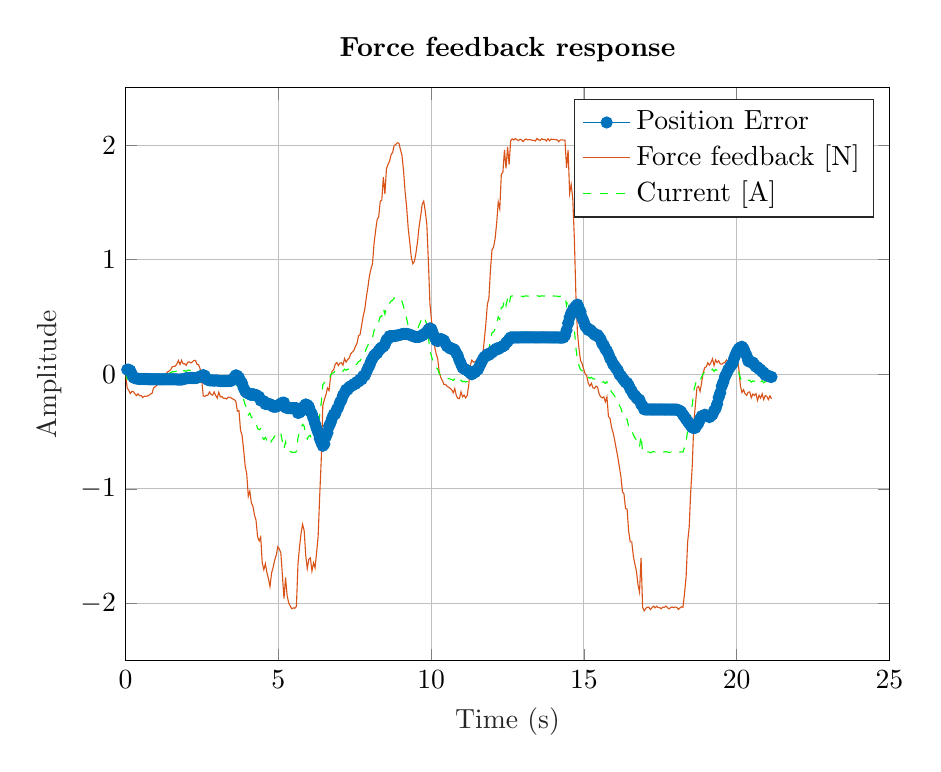
\begin{tikzpicture}

\begin{axis}[%
width=0.8\columnwidth,
height=0.6\columnwidth,
at={(2.512in,1.147in)},
scale only axis,
unbounded coords=jump,
xmin=0,
xmax=25,
xlabel style={font=\color{white!15!black}},
xlabel={Time (s)},
ymin=-2.5,
ymax=2.5,
ylabel style={font=\color{white!15!black}},
ylabel={Amplitude},
axis background/.style={fill=white},
title style={font=\bfseries},
title={Force feedback response},
xmajorgrids,
ymajorgrids,
legend style={legend cell align=left, align=left, draw=white!15!black}
]
\addplot [color=mycolor1, draw=none, mark=*, mark options={solid, mycolor1}]
  table[row sep=crcr]{%
0	nan\\
0.0508143901824951	0.040583486\\
0.10162878036499	0.040390871\\
0.152443170547485	0.0311559\\
0.20325756072998	0.000476299999999999\\
0.254071950912476	-0.0268124\\
0.304886341094971	-0.0342713\\
0.355700731277466	-0.03624\\
0.406515121459961	-0.0391465\\
0.457329511642456	-0.0405998\\
0.508143901824951	-0.0405998\\
0.558958292007446	-0.0405998\\
0.609772682189941	-0.0408916\\
0.660587072372437	-0.0408916\\
0.711401462554932	-0.041376\\
0.762215852737427	-0.0433137\\
0.813030242919922	-0.0433137\\
0.863844633102417	-0.0433137\\
0.914659023284912	-0.0433137\\
0.965473413467407	-0.0433137\\
1.0162878036499	-0.0433137\\
1.0671021938324	-0.0436055\\
1.11791658401489	-0.0438973\\
1.16873097419739	-0.0438973\\
1.21954536437988	-0.0438973\\
1.27035975456238	-0.0436055\\
1.32117414474487	-0.0436055\\
1.37198853492737	-0.0436055\\
1.42280292510986	-0.0436055\\
1.47361731529236	-0.043444\\
1.52443170547485	-0.043444\\
1.57524609565735	-0.043444\\
1.62606048583984	-0.0432825\\
1.67687487602234	-0.0450332\\
1.72768926620483	-0.0460389\\
1.77850365638733	-0.0453053\\
1.82931804656982	-0.0459625\\
1.88013243675232	-0.0421921\\
1.93094682693481	-0.0389003\\
1.98176121711731	-0.0347332\\
2.0325756072998	-0.0336029\\
2.0833899974823	-0.032634\\
2.13420438766479	-0.032634\\
2.18501877784729	-0.032634\\
2.23583316802979	-0.032634\\
2.28664755821228	-0.032634\\
2.33746194839478	-0.0296596\\
2.38827633857727	-0.0255746\\
2.43909072875977	-0.0201921\\
2.48990511894226	-0.0145179\\
2.54071950912476	-0.0069625\\
2.59153389930725	-0.0136706\\
2.64234828948975	-0.0365684\\
2.69316267967224	-0.0494236\\
2.74397706985474	-0.052231\\
2.79479146003723	-0.0535542\\
2.84560585021973	-0.0532625\\
2.89642024040222	-0.0552307\\
2.94723463058472	-0.053152\\
2.99804902076721	-0.0530524\\
3.04886341094971	-0.0577354\\
3.0996778011322	-0.0591572\\
3.1504921913147	-0.0591572\\
3.20130658149719	-0.0591572\\
3.25212097167969	-0.0591572\\
3.30293536186218	-0.0588654\\
3.35374975204468	-0.0580525\\
3.40456414222717	-0.0589219\\
3.45537853240967	-0.0569047\\
3.50619292259216	-0.0423154\\
3.55700731277466	-0.027021\\
3.60782170295715	-0.008766\\
3.65863609313965	-0.014097\\
3.70945048332214	-0.030031\\
3.76026487350464	-0.058569\\
3.81107926368713	-0.077869\\
3.86189365386963	-0.119089\\
3.91270804405212	-0.146783\\
3.96352243423462	-0.161049\\
4.01433682441711	-0.164225\\
4.06515121459961	-0.173349\\
4.1159656047821	-0.18127\\
4.1667799949646	-0.172498\\
4.21759438514709	-0.181538\\
4.26840877532959	-0.179804\\
4.31922316551208	-0.191297\\
4.37003755569458	-0.197869\\
4.42085194587708	-0.228469\\
4.47166633605957	-0.232812\\
4.52248072624207	-0.235036\\
4.57329511642456	-0.25948\\
4.62410950660706	-0.25948\\
4.67492389678955	-0.259803\\
4.72573828697205	-0.260449\\
4.77655267715454	-0.269814\\
4.82736706733704	-0.282409\\
4.87818145751953	-0.282409\\
4.92899584770203	-0.282118\\
4.97981023788452	-0.276282\\
5.03062462806702	-0.266653\\
5.08143901824951	-0.254981\\
5.13225340843201	-0.247979\\
5.1830677986145	-0.247389\\
5.233882188797	-0.287918\\
5.28469657897949	-0.2947\\
5.33551096916199	-0.295023\\
5.38632535934448	-0.295508\\
5.43713974952698	-0.295669\\
5.48795413970947	-0.295669\\
5.53876852989197	-0.295831\\
5.58958292007446	-0.295539\\
5.64039731025696	-0.337198\\
5.69121170043945	-0.333405\\
5.74202609062195	-0.320566\\
5.79284048080444	-0.301017\\
5.84365487098694	-0.278549\\
5.89446926116943	-0.262793\\
5.94528365135193	-0.268649\\
5.99609804153442	-0.282347\\
6.04691243171692	-0.323013\\
6.09772682189941	-0.346548\\
6.14854121208191	-0.386557\\
6.1993556022644	-0.42999\\
6.2501699924469	-0.472591\\
6.30098438262939	-0.507897\\
6.35179877281189	-0.561003\\
6.40261316299438	-0.594558\\
6.45342755317688	-0.624151\\
6.50424194335938	-0.608321\\
6.55505633354187	-0.54348\\
6.60587072372437	-0.5107469\\
6.65668511390686	-0.4528868\\
6.70749950408936	-0.4231707\\
6.75831389427185	-0.3834065\\
6.80912828445435	-0.3516815\\
6.85994267463684	-0.34493987\\
6.91075706481934	-0.3077656\\
6.96157145500183	-0.2868116\\
7.01238584518433	-0.2466247\\
7.06320023536682	-0.2251016\\
7.11401462554932	-0.1844754\\
7.16482901573181	-0.1635496\\
7.21564340591431	-0.134754\\
7.2664577960968	-0.1332392\\
7.3172721862793	-0.11288174\\
7.36808657646179	-0.1037071\\
7.41890096664429	-0.0974778\\
7.46971535682678	-0.0850794\\
7.52052974700928	-0.08391\\
7.57134413719177	-0.067102\\
7.62215852737427	-0.063412\\
7.67297291755676	-0.045387\\
7.72378730773926	-0.044334\\
7.77460169792175	-0.015388\\
7.82541608810425	-0.010635\\
7.87623047828674	0.018081\\
7.92704486846924	0.051138\\
7.97785925865173	0.074857\\
8.02867364883423	0.111797\\
8.07948803901672	0.136825\\
8.13030242919922	0.161369\\
8.18111681938171	0.17549\\
8.23193120956421	0.185346\\
8.2827455997467	0.206088\\
8.3335599899292	0.223054\\
8.38437438011169	0.235045\\
8.43518877029419	0.242634\\
8.48600316047668	0.260011\\
8.53681755065918	0.299249\\
8.58763194084167	0.309421\\
8.63844633102417	0.332673\\
8.68926072120667	0.332996\\
8.74007511138916	0.333741\\
8.79088950157166	0.335361\\
8.84170389175415	0.336528\\
8.89251828193665	0.338571\\
8.94333267211914	0.342364\\
8.99414706230164	0.345574\\
9.04496145248413	0.350242\\
9.09577584266663	0.352285\\
9.14659023284912	0.352285\\
9.19740462303162	0.352285\\
9.24821901321411	0.349498\\
9.29903340339661	0.345996\\
9.3498477935791	0.34029\\
9.4006621837616	0.334585\\
9.45147657394409	0.327874\\
9.50229096412659	0.326707\\
9.55310535430908	0.326415\\
9.60391974449158	0.326999\\
9.65473413467407	0.332543\\
9.70554852485657	0.338379\\
9.75636291503906	0.349467\\
9.80717730522156	0.357053\\
9.85799169540405	0.370183\\
9.90880608558655	0.389441\\
9.95962047576904	0.401113\\
10.0104348659515	0.393025\\
10.061249256134	0.356053\\
10.1120636463165	0.323989\\
10.162878036499	0.297009\\
10.2136924266815	0.290058\\
10.264506816864	0.297244\\
10.3153212070465	0.308417\\
10.366135597229	0.302251\\
10.4169499874115	0.29452\\
10.467764377594	0.270257\\
10.5185787677765	0.245764\\
10.569393157959	0.238884\\
10.6202075481415	0.225488\\
10.671021938324	0.221885\\
10.7218363285065	0.2212201\\
10.772650718689	0.2104693\\
10.8234651088715	0.1847531\\
10.874279499054	0.1603938\\
10.9250938892365	0.1209552\\
10.9759082794189	0.0912297\\
11.0267226696014	0.0590041\\
11.0775370597839	0.0485706\\
11.1283514499664	0.0414176\\
11.1791658401489	0.0339614\\
11.2299802303314	0.0249161\\
11.2807946205139	0.0109415\\
11.3316090106964	0.00018\\
11.3824234008789	0.016117\\
11.4332377910614	0.01702\\
11.4840521812439	0.035169\\
11.5348665714264	0.043953\\
11.5856809616089	0.074499\\
11.6364953517914	0.099936\\
11.6873097419739	0.12845\\
11.7381241321564	0.150425\\
11.7889385223389	0.1582\\
11.8397529125214	0.174709\\
11.8905673027039	0.169726\\
11.9413816928864	0.185867\\
11.9921960830688	0.190697\\
12.0430104732513	0.206431\\
12.0938248634338	0.211773\\
12.1446392536163	0.224959\\
12.1954536437988	0.220322\\
12.2462680339813	0.233812\\
12.2970824241638	0.237446\\
12.3478968143463	0.244452\\
12.3987112045288	0.25288\\
12.4495255947113	0.273871\\
12.5003399848938	0.285497\\
12.5511543750763	0.304228\\
12.6019687652588	0.321667\\
12.6527831554413	0.321667\\
12.7035975456238	0.321828\\
12.7544119358063	0.321828\\
12.8052263259888	0.321828\\
12.8560407161713	0.321828\\
12.9068551063538	0.32212\\
12.9576694965363	0.322411\\
13.0084838867188	0.322411\\
13.0592982769012	0.322411\\
13.1101126670837	0.322411\\
13.1609270572662	0.322411\\
13.2117414474487	0.322411\\
13.2625558376312	0.322411\\
13.3133702278137	0.322411\\
13.3641846179962	0.322411\\
13.4149990081787	0.32212\\
13.4658133983612	0.32212\\
13.5166277885437	0.32212\\
13.5674421787262	0.32212\\
13.6182565689087	0.322411\\
13.6690709590912	0.322411\\
13.7198853492737	0.322411\\
13.7706997394562	0.32212\\
13.8215141296387	0.32212\\
13.8723285198212	0.32212\\
13.9231429100037	0.321828\\
13.9739573001862	0.321828\\
14.0247716903687	0.321828\\
14.0755860805511	0.321828\\
14.1264004707336	0.321828\\
14.1772148609161	0.321536\\
14.2280292510986	0.320077\\
14.2788436412811	0.320369\\
14.3296580314636	0.321536\\
14.3804724216461	0.338845\\
14.4312868118286	0.384845\\
14.4821012020111	0.445114\\
14.5329155921936	0.498029\\
14.5837299823761	0.535446\\
14.6345443725586	0.556455\\
14.6853587627411	0.578339\\
14.7361731529236	0.594225\\
14.7869875431061	0.608372\\
14.8378019332886	0.57582\\
14.8886163234711	0.545835\\
14.9394307136536	0.493691\\
14.9902451038361	0.462122\\
15.0410594940186	0.42246\\
15.091873884201	0.406649\\
15.1426882743835	0.386664\\
15.193502664566	0.390257\\
15.2443170547485	0.377604\\
15.295131444931	0.3630856\\
15.3459458351135	0.3480997\\
15.396760225296	0.338608\\
15.4475746154785	0.34282107\\
15.498389005661	0.3233764\\
15.5492033958435	0.304621\\
15.600017786026	0.266437\\
15.6508321762085	0.254336\\
15.701646566391	0.2208409\\
15.7524609565735	0.2048468\\
15.803275346756	0.17702373\\
15.8540897369385	0.1404687\\
15.904904127121	0.1187586\\
15.9557185173035	0.087172\\
16.006532907486	0.072578\\
16.0573472976685	0.049791\\
16.108161687851	0.035707\\
16.1589760780334	-0.00040399999999996\\
16.2097904682159	-0.012885\\
16.2606048583984	-0.032746\\
16.3114192485809	-0.050281\\
16.3622336387634	-0.068699\\
16.4130480289459	-0.074883\\
16.4638624191284	-0.095201\\
16.5146768093109	-0.126279\\
16.5654911994934	-0.146333\\
16.6163055896759	-0.172684\\
16.6671199798584	-0.184956\\
16.7179343700409	-0.204978\\
16.7687487602234	-0.215635\\
16.8195631504059	-0.223709\\
16.8703775405884	-0.260686\\
16.9211919307709	-0.276026\\
16.9720063209534	-0.305898\\
17.0228207111359	-0.306965\\
17.0736351013184	-0.306965\\
17.1244494915009	-0.306965\\
17.1752638816833	-0.307257\\
17.2260782718658	-0.307257\\
17.2768926620483	-0.307257\\
17.3277070522308	-0.307257\\
17.3785214424133	-0.307257\\
17.4293358325958	-0.307257\\
17.4801502227783	-0.307257\\
17.5309646129608	-0.307257\\
17.5817790031433	-0.307257\\
17.6325933933258	-0.307549\\
17.6834077835083	-0.307549\\
17.7342221736908	-0.307549\\
17.7850365638733	-0.307549\\
17.8358509540558	-0.307841\\
17.8866653442383	-0.307841\\
17.9374797344208	-0.307841\\
17.9882941246033	-0.308003\\
18.0391085147858	-0.308003\\
18.0899229049683	-0.31238\\
18.1407372951508	-0.319674\\
18.1915516853333	-0.329887\\
18.2423660755157	-0.35323\\
18.2931804656982	-0.371612\\
18.3439948558807	-0.391454\\
18.3948092460632	-0.410128\\
18.4456236362457	-0.429094\\
18.4964380264282	-0.446601\\
18.5472524166107	-0.463947\\
18.5980668067932	-0.469659\\
18.6488811969757	-0.466103\\
18.6996955871582	-0.44126\\
18.7505099773407	-0.425339\\
18.8013243675232	-0.39075\\
18.8521387577057	-0.365842\\
18.9029531478882	-0.36368\\
18.9537675380707	-0.352947\\
19.0045819282532	-0.3586815\\
19.0553963184357	-0.3630554\\
19.1062107086182	-0.37384626\\
19.1570250988007	-0.3621307\\
19.2078394889832	-0.3507551\\
19.2586538791656	-0.318937\\
19.3094682693481	-0.300414\\
19.3602826595306	-0.2594797\\
19.4110970497131	-0.2013389\\
19.4619114398956	-0.1620305\\
19.5127258300781	-0.1028439\\
19.5635402202606	-0.06732\\
19.6143546104431	-0.021947\\
19.6651690006256	0.00479599999999999\\
19.7159833908081	0.03745\\
19.7667977809906	0.057155\\
19.8176121711731	0.078954\\
19.8684265613556	0.095168\\
19.9192409515381	0.140944\\
19.9700553417206	0.17606\\
20.0208697319031	0.203749\\
20.0716841220856	0.223615\\
20.1224985122681	0.235126\\
20.1733129024506	0.240159\\
20.2241272926331	0.2225424\\
20.2749416828156	0.1911464\\
20.325756072998	0.1617559\\
20.3765704631805	0.117119\\
20.427384853363	0.1086436\\
20.4781992435455	0.1076383\\
20.529013633728	0.1024425\\
20.5798280239105	0.0830015\\
20.630642414093	0.0668373\\
20.6814568042755	0.06150592\\
20.732271194458	0.04705583\\
20.7830855846405	0.03958864\\
20.833899974823	0.02269947\\
20.8847143650055	0.01466835\\
20.935528755188	-0.0050566\\
20.9863431453705	-0.0099262\\
21.037157535553	-0.0143794\\
21.0879719257355	-0.0206456\\
21.138786315918	-0.0232291\\
};
\addlegendentry{Position Error}

\addplot [color=mycolor2]
  table[row sep=crcr]{%
0	-0\\
0.0508143901824951	-0.120667\\
0.10162878036499	-0.13888\\
0.152443170547485	-0.168594\\
0.20325756072998	-0.14942\\
0.254071950912476	-0.152298\\
0.304886341094971	-0.170511\\
0.355700731277466	-0.185846\\
0.406515121459961	-0.170511\\
0.457329511642456	-0.186802\\
0.508143901824951	-0.185846\\
0.558958292007446	-0.202143\\
0.609772682189941	-0.191597\\
0.660587072372437	-0.192558\\
0.711401462554932	-0.18968\\
0.762215852737427	-0.184885\\
0.813030242919922	-0.171467\\
0.863844633102417	-0.165716\\
0.914659023284912	-0.119705\\
0.965473413467407	-0.108204\\
1.0162878036499	-0.0976639\\
1.0671021938324	-0.0775337\\
1.11791658401489	-0.066988\\
1.16873097419739	-0.0554867\\
1.21954536437988	-0.0305672\\
1.27035975456238	-0.0171432\\
1.32117414474487	0.00394249\\
1.37198853492737	0.0211945\\
1.42280292510986	0.0279064\\
1.47361731529236	0.0394077\\
1.52443170547485	0.0652885\\
1.57524609565735	0.0691223\\
1.62606048583984	0.0710392\\
1.67687487602234	0.0902081\\
1.72768926620483	0.119923\\
1.77850365638733	0.0854187\\
1.82931804656982	0.12184\\
1.88013243675232	0.0911694\\
1.93094682693481	0.0930862\\
1.98176121711731	0.0777512\\
2.0325756072998	0.106504\\
2.0833899974823	0.108421\\
2.13420438766479	0.0988369\\
2.18501877784729	0.10746\\
2.23583316802979	0.12184\\
2.28664755821228	0.120884\\
2.33746194839478	0.0863743\\
2.38827633857727	0.0835018\\
2.43909072875977	0.0470753\\
2.48990511894226	-0.0535698\\
2.54071950912476	-0.187763\\
2.59153389930725	-0.193514\\
2.64234828948975	-0.183929\\
2.69316267967224	-0.182013\\
2.74397706985474	-0.154215\\
2.79479146003723	-0.175301\\
2.84560585021973	-0.182013\\
2.89642024040222	-0.154215\\
2.94723463058472	-0.182968\\
2.99804902076721	-0.207893\\
3.04886341094971	-0.157093\\
3.0996778011322	-0.198309\\
3.1504921913147	-0.194475\\
3.20130658149719	-0.20981\\
3.25212097167969	-0.208849\\
3.30293536186218	-0.215561\\
3.35374975204468	-0.200226\\
3.40456414222717	-0.199265\\
3.45537853240967	-0.205976\\
3.50619292259216	-0.215561\\
3.55700731277466	-0.221312\\
3.60782170295715	-0.236647\\
3.65863609313965	-0.321957\\
3.70945048332214	-0.317162\\
3.76026487350464	-0.487782\\
3.81107926368713	-0.532831\\
3.86189365386963	-0.658401\\
3.91270804405212	-0.801218\\
3.96352243423462	-0.868315\\
4.01433682441711	-1.06482\\
4.06515121459961	-1.0188\\
4.1159656047821	-1.12328\\
4.1667799949646	-1.153\\
4.21759438514709	-1.22872\\
4.26840877532959	-1.27473\\
4.31922316551208	-1.41755\\
4.37003755569458	-1.45398\\
4.42085194587708	-1.42043\\
4.47166633605957	-1.64472\\
4.52248072624207	-1.70511\\
4.57329511642456	-1.65335\\
4.62410950660706	-1.73099\\
4.67492389678955	-1.78563\\
4.72573828697205	-1.85272\\
4.77655267715454	-1.73483\\
4.82736706733704	-1.68594\\
4.87818145751953	-1.62076\\
4.92899584770203	-1.57954\\
4.97981023788452	-1.50574\\
5.03062462806702	-1.52395\\
5.08143901824951	-1.56229\\
5.13225340843201	-1.7607\\
5.1830677986145	-1.9572\\
5.233882188797	-1.77316\\
5.28469657897949	-1.93037\\
5.33551096916199	-1.99459\\
5.38632535934448	-2.02142\\
5.43713974952698	-2.04539\\
5.48795413970947	-2.03868\\
5.53876852989197	-2.04155\\
5.58958292007446	-2.02622\\
5.64039731025696	-1.6591\\
5.69121170043945	-1.50766\\
5.74202609062195	-1.38784\\
5.79284048080444	-1.3102\\
5.84365487098694	-1.36483\\
5.89446926116943	-1.58146\\
5.94528365135193	-1.69552\\
5.99609804153442	-1.61501\\
6.04691243171692	-1.60255\\
6.09772682189941	-1.71757\\
6.14854121208191	-1.64568\\
6.1993556022644	-1.68882\\
6.2501699924469	-1.5575\\
6.30098438262939	-1.41276\\
6.35179877281189	-1.06194\\
6.40261316299438	-0.743706\\
6.45342755317688	-0.274029\\
6.50424194335938	-0.220356\\
6.55505633354187	-0.180096\\
6.60587072372437	-0.119705\\
6.65668511390686	-0.141752\\
6.70749950408936	-0.0238552\\
6.75831389427185	0.0269451\\
6.80912828445435	0.0403633\\
6.85994267463684	0.0873356\\
6.91075706481934	0.102671\\
6.96157145500183	0.0767899\\
7.01238584518433	0.0978756\\
7.06320023536682	0.100754\\
7.11401462554932	0.079668\\
7.16482901573181	0.137175\\
7.21564340591431	0.106504\\
7.2664577960968	0.128551\\
7.3172721862793	0.141008\\
7.36808657646179	0.179352\\
7.41890096664429	0.193731\\
7.46971535682678	0.208111\\
7.52052974700928	0.243576\\
7.57134413719177	0.268496\\
7.62215852737427	0.336548\\
7.67297291755676	0.346138\\
7.72378730773926	0.424736\\
7.77460169792175	0.507168\\
7.82541608810425	0.56468\\
7.87623047828674	0.669159\\
7.92704486846924	0.755424\\
7.97785925865173	0.85607\\
8.02867364883423	0.919333\\
8.07948803901672	0.963427\\
8.13030242919922	1.1398\\
8.18111681938171	1.2529\\
8.23193120956421	1.34971\\
8.2827455997467	1.37464\\
8.3335599899292	1.50883\\
8.38437438011169	1.52129\\
8.43518877029419	1.72162\\
8.48600316047668	1.57401\\
8.53681755065918	1.79351\\
8.58763194084167	1.83281\\
8.63844633102417	1.85965\\
8.68926072120667	1.91716\\
8.74007511138916	1.93729\\
8.79088950157166	1.99767\\
8.84170389175415	2.0063\\
8.89251828193665	2.02068\\
8.94333267211914	2.01781\\
8.99414706230164	1.96221\\
9.04496145248413	1.91045\\
9.09577584266663	1.77722\\
9.14659023284912	1.59606\\
9.19740462303162	1.45803\\
9.24821901321411	1.27686\\
9.29903340339661	1.15417\\
9.3498477935791	1.02189\\
9.4006621837616	0.964388\\
9.45147657394409	0.984512\\
9.50229096412659	1.05832\\
9.55310535430908	1.15513\\
9.60391974449158	1.28836\\
9.65473413467407	1.37655\\
9.70554852485657	1.4839\\
9.75636291503906	1.5117\\
9.80717730522156	1.42256\\
9.85799169540405	1.30754\\
9.90880608558655	0.987391\\
9.95962047576904	0.616442\\
10.0104348659515	0.473619\\
10.061249256134	0.339426\\
10.1120636463165	0.244532\\
10.162878036499	0.179352\\
10.2136924266815	0.136219\\
10.264506816864	0.018322\\
10.3153212070465	-0.027689\\
10.366135597229	-0.0535698\\
10.4169499874115	-0.089035\\
10.467764377594	-0.0880737\\
10.5185787677765	-0.103415\\
10.569393157959	-0.112999\\
10.6202075481415	-0.122583\\
10.671021938324	-0.135046\\
10.7218363285065	-0.161882\\
10.772650718689	-0.1245\\
10.8234651088715	-0.184885\\
10.874279499054	-0.210766\\
10.9250938892365	-0.212683\\
10.9759082794189	-0.153254\\
11.0267226696014	-0.196392\\
11.0775370597839	-0.182013\\
11.1283514499664	-0.205976\\
11.1791658401489	-0.185846\\
11.2299802303314	-0.0947857\\
11.2807946205139	0.0767899\\
11.3316090106964	0.123756\\
11.3824234008789	0.10746\\
11.4332377910614	0.106504\\
11.4840521812439	0.123756\\
11.5348665714264	0.10746\\
11.5856809616089	0.115133\\
11.6364953517914	0.118967\\
11.6873097419739	0.164972\\
11.7381241321564	0.296293\\
11.7889385223389	0.436237\\
11.8397529125214	0.60973\\
11.8905673027039	0.665325\\
11.9413816928864	0.914543\\
11.9921960830688	1.08612\\
12.0430104732513	1.11104\\
12.0938248634338	1.1858\\
12.1446392536163	1.32191\\
12.1954536437988	1.50403\\
12.2462680339813	1.4446\\
12.2970824241638	1.7475\\
12.3478968143463	1.76284\\
12.3987112045288	1.95742\\
12.4495255947113	1.79735\\
12.5003399848938	1.98522\\
12.5511543750763	1.82993\\
12.6019687652588	2.03889\\
12.6527831554413	2.05423\\
12.7035975456238	2.0456\\
12.7544119358063	2.05807\\
12.8052263259888	2.04752\\
12.8560407161713	2.04081\\
12.9068551063538	2.0504\\
12.9576694965363	2.0456\\
13.0084838867188	2.03027\\
13.0592982769012	2.04848\\
13.1101126670837	2.05327\\
13.1609270572662	2.0456\\
13.2117414474487	2.04944\\
13.2625558376312	2.0456\\
13.3133702278137	2.04272\\
13.3641846179962	2.04177\\
13.4149990081787	2.03602\\
13.4658133983612	2.05902\\
13.5166277885437	2.04656\\
13.5674421787262	2.04081\\
13.6182565689087	2.05615\\
13.6690709590912	2.04848\\
13.7198853492737	2.0504\\
13.7706997394562	2.03602\\
13.8215141296387	2.05615\\
13.8723285198212	2.03794\\
13.9231429100037	2.05327\\
13.9739573001862	2.04944\\
14.0247716903687	2.0504\\
14.0755860805511	2.04752\\
14.1264004707336	2.04656\\
14.1772148609161	2.03027\\
14.2280292510986	2.0456\\
14.2788436412811	2.04656\\
14.3296580314636	2.04369\\
14.3804724216461	2.04272\\
14.4312868118286	1.80214\\
14.4821012020111	1.95742\\
14.5329155921936	1.57976\\
14.5837299823761	1.6574\\
14.6345443725586	1.53471\\
14.6853587627411	1.19635\\
14.7361731529236	0.70079\\
14.7869875431061	0.368179\\
14.8378019332886	0.226318\\
14.8886163234711	0.12184\\
14.9394307136536	0.0950031\\
14.9902451038361	0.0461197\\
15.0410594940186	0.00394249\\
15.091873884201	-0.0123539\\
15.1426882743835	-0.0775337\\
15.193502664566	-0.102453\\
15.2443170547485	-0.0784893\\
15.295131444931	-0.117788\\
15.3459458351135	-0.123545\\
15.396760225296	-0.102453\\
15.4475746154785	-0.112038\\
15.498389005661	-0.172428\\
15.5492033958435	-0.196392\\
15.600017786026	-0.205976\\
15.6508321762085	-0.196392\\
15.701646566391	-0.24048\\
15.7524609565735	-0.196392\\
15.803275346756	-0.368923\\
15.8540897369385	-0.384258\\
15.904904127121	-0.465734\\
15.9557185173035	-0.507912\\
16.006532907486	-0.575964\\
16.0573472976685	-0.649773\\
16.108161687851	-0.720703\\
16.1589760780334	-0.80793\\
16.2097904682159	-0.889406\\
16.2606048583984	-1.02456\\
16.3114192485809	-1.04565\\
16.3622336387634	-1.17217\\
16.4130480289459	-1.17601\\
16.4638624191284	-1.36962\\
16.5146768093109	-1.46165\\
16.5654911994934	-1.4626\\
16.6163055896759	-1.58338\\
16.6671199798584	-1.65622\\
16.7179343700409	-1.71757\\
16.7687487602234	-1.83451\\
16.8195631504059	-1.90161\\
16.8703775405884	-1.60159\\
16.9211919307709	-2.03293\\
16.9720063209534	-2.06456\\
17.0228207111359	-2.04347\\
17.0736351013184	-2.03388\\
17.1244494915009	-2.03197\\
17.1752638816833	-2.05305\\
17.2260782718658	-2.03772\\
17.2768926620483	-2.02334\\
17.3277070522308	-2.03772\\
17.3785214424133	-2.0243\\
17.4293358325958	-2.0358\\
17.4801502227783	-2.03676\\
17.5309646129608	-2.04635\\
17.5817790031433	-2.03197\\
17.6325933933258	-2.03388\\
17.6834077835083	-2.02334\\
17.7342221736908	-2.03676\\
17.7850365638733	-2.0473\\
17.8358509540558	-2.0358\\
17.8866653442383	-2.03101\\
17.9374797344208	-2.03676\\
17.9882941246033	-2.03101\\
18.0391085147858	-2.03485\\
18.0899229049683	-2.0521\\
18.1407372951508	-2.03963\\
18.1915516853333	-2.02909\\
18.2423660755157	-2.03388\\
18.2931804656982	-1.91024\\
18.3439948558807	-1.77125\\
18.3948092460632	-1.46356\\
18.4456236362457	-1.3332\\
18.4964380264282	-1.0188\\
18.5472524166107	-0.792595\\
18.5980668067932	-0.41589\\
18.6488811969757	-0.266361\\
18.6996955871582	-0.116833\\
18.7505099773407	-0.105331\\
18.8013243675232	-0.14942\\
18.8521387577057	-0.0746555\\
18.9029531478882	0.0154438\\
18.9537675380707	0.0566597\\
19.0045819282532	0.0652885\\
19.0553963184357	0.100754\\
19.1062107086182	0.079668\\
19.1570250988007	0.101709\\
19.2078394889832	0.135258\\
19.2586538791656	0.0767899\\
19.3094682693481	0.126635\\
19.3602826595306	0.102671\\
19.4110970497131	0.118006\\
19.4619114398956	0.0911694\\
19.5127258300781	0.0882912\\
19.5635402202606	0.0997925\\
19.6143546104431	0.101709\\
19.6651690006256	0.125673\\
19.7159833908081	0.1113\\
19.7667977809906	0.1113\\
19.8176121711731	0.145803\\
19.8684265613556	0.161139\\
19.9192409515381	0.122801\\
19.9700553417206	0.129507\\
20.0208697319031	0.135258\\
20.0716841220856	0.0451584\\
20.1224985122681	-0.102453\\
20.1733129024506	-0.15901\\
20.2241272926331	-0.135046\\
20.2749416828156	-0.170511\\
20.325756072998	-0.182968\\
20.3765704631805	-0.156132\\
20.427384853363	-0.154215\\
20.4781992435455	-0.205015\\
20.529013633728	-0.172428\\
20.5798280239105	-0.183929\\
20.630642414093	-0.168594\\
20.6814568042755	-0.228024\\
20.732271194458	-0.182968\\
20.7830855846405	-0.207893\\
20.833899974823	-0.170511\\
20.8847143650055	-0.220356\\
20.935528755188	-0.185846\\
20.9863431453705	-0.192558\\
21.037157535553	-0.220356\\
21.0879719257355	-0.187763\\
21.138786315918	-0.213644\\
};
\addlegendentry{Force feedback [N]}

\addplot [color=green, dashed]
  table[row sep=crcr]{%
0	0\\
0.0508143901824951	-0.0402222\\
0.10162878036499	-0.0462933\\
0.152443170547485	-0.0561981\\
0.20325756072998	-0.0498066\\
0.254071950912476	-0.050766\\
0.304886341094971	-0.0568371\\
0.355700731277466	-0.0619488\\
0.406515121459961	-0.0568371\\
0.457329511642456	-0.0622673\\
0.508143901824951	-0.0619488\\
0.558958292007446	-0.0673809\\
0.609772682189941	-0.0638657\\
0.660587072372437	-0.0641861\\
0.711401462554932	-0.0632267\\
0.762215852737427	-0.0616283\\
0.813030242919922	-0.0571556\\
0.863844633102417	-0.0552387\\
0.914659023284912	-0.0399017\\
0.965473413467407	-0.036068\\
1.0162878036499	-0.0325546\\
1.0671021938324	-0.0258446\\
1.11791658401489	-0.0223293\\
1.16873097419739	-0.0184956\\
1.21954536437988	-0.0101891\\
1.27035975456238	-0.00571442\\
1.32117414474487	0.00131416\\
1.37198853492737	0.00706482\\
1.42280292510986	0.00930214\\
1.47361731529236	0.0131359\\
1.52443170547485	0.0217628\\
1.57524609565735	0.0230408\\
1.62606048583984	0.0236797\\
1.67687487602234	0.0300694\\
1.72768926620483	0.0399742\\
1.77850365638733	0.0284729\\
1.82931804656982	0.0406132\\
1.88013243675232	0.0303898\\
1.93094682693481	0.0310287\\
1.98176121711731	0.0259171\\
2.0325756072998	0.0355015\\
2.0833899974823	0.0361404\\
2.13420438766479	0.0329456\\
2.18501877784729	0.03582\\
2.23583316802979	0.0406132\\
2.28664755821228	0.0402946\\
2.33746194839478	0.0287914\\
2.38827633857727	0.0278339\\
2.43909072875977	0.0156918\\
2.48990511894226	-0.0178566\\
2.54071950912476	-0.0625877\\
2.59153389930725	-0.0645046\\
2.64234828948975	-0.0613098\\
2.69316267967224	-0.0606709\\
2.74397706985474	-0.051405\\
2.79479146003723	-0.0584335\\
2.84560585021973	-0.0606709\\
2.89642024040222	-0.051405\\
2.94723463058472	-0.0609894\\
2.99804902076721	-0.0692978\\
3.04886341094971	-0.0523643\\
3.0996778011322	-0.066103\\
3.1504921913147	-0.0648251\\
3.20130658149719	-0.0699368\\
3.25212097167969	-0.0696163\\
3.30293536186218	-0.0718536\\
3.35374975204468	-0.0667419\\
3.40456414222717	-0.0664215\\
3.45537853240967	-0.0686588\\
3.50619292259216	-0.0718536\\
3.55700731277466	-0.0737705\\
3.60782170295715	-0.0788822\\
3.65863609313965	-0.107319\\
3.70945048332214	-0.105721\\
3.76026487350464	-0.162594\\
3.81107926368713	-0.17761\\
3.86189365386963	-0.219467\\
3.91270804405212	-0.267073\\
3.96352243423462	-0.289438\\
4.01433682441711	-0.354939\\
4.06515121459961	-0.339602\\
4.1159656047821	-0.374428\\
4.1667799949646	-0.384333\\
4.21759438514709	-0.409575\\
4.26840877532959	-0.424911\\
4.31922316551208	-0.472517\\
4.37003755569458	-0.484659\\
4.42085194587708	-0.473476\\
4.47166633605957	-0.548241\\
4.52248072624207	-0.568371\\
4.57329511642456	-0.551117\\
4.62410950660706	-0.576996\\
4.67492389678955	-0.595209\\
4.72573828697205	-0.617575\\
4.77655267715454	-0.578276\\
4.82736706733704	-0.561979\\
4.87818145751953	-0.540253\\
4.92899584770203	-0.526514\\
4.97981023788452	-0.501913\\
5.03062462806702	-0.507982\\
5.08143901824951	-0.520763\\
5.13225340843201	-0.586901\\
5.1830677986145	-0.652401\\
5.233882188797	-0.591055\\
5.28469657897949	-0.643456\\
5.33551096916199	-0.664862\\
5.38632535934448	-0.673807\\
5.43713974952698	-0.681795\\
5.48795413970947	-0.67956\\
5.53876852989197	-0.680517\\
5.58958292007446	-0.675406\\
5.64039731025696	-0.553034\\
5.69121170043945	-0.502552\\
5.74202609062195	-0.462612\\
5.79284048080444	-0.436733\\
5.84365487098694	-0.454945\\
5.89446926116943	-0.527153\\
5.94528365135193	-0.565174\\
5.99609804153442	-0.538336\\
6.04691243171692	-0.534184\\
6.09772682189941	-0.572523\\
6.14854121208191	-0.548561\\
6.1993556022644	-0.562939\\
6.2501699924469	-0.519165\\
6.30098438262939	-0.470921\\
6.35179877281189	-0.353979\\
6.40261316299438	-0.247902\\
6.45342755317688	-0.0913429\\
6.50424194335938	-0.073452\\
6.55505633354187	-0.0600319\\
6.60587072372437	-0.0399017\\
6.65668511390686	-0.0472507\\
6.70749950408936	-0.00795174\\
6.75831389427185	0.0089817\\
6.80912828445435	0.0134544\\
6.85994267463684	0.0291119\\
6.91075706481934	0.0342236\\
6.96157145500183	0.0255966\\
7.01238584518433	0.0326252\\
7.06320023536682	0.0335846\\
7.11401462554932	0.026556\\
7.16482901573181	0.0457249\\
7.21564340591431	0.0355015\\
7.2664577960968	0.0428505\\
7.3172721862793	0.0470028\\
7.36808657646179	0.0597839\\
7.41890096664429	0.0645771\\
7.46971535682678	0.0693703\\
7.52052974700928	0.081192\\
7.57134413719177	0.0894985\\
7.62215852737427	0.112183\\
7.67297291755676	0.115379\\
7.72378730773926	0.141579\\
7.77460169792175	0.169056\\
7.82541608810425	0.188227\\
7.87623047828674	0.223053\\
7.92704486846924	0.251808\\
7.97785925865173	0.285357\\
8.02867364883423	0.306444\\
8.07948803901672	0.321142\\
8.13030242919922	0.379932\\
8.18111681938171	0.417633\\
8.23193120956421	0.449903\\
8.2827455997467	0.458212\\
8.3335599899292	0.502943\\
8.38437438011169	0.507097\\
8.43518877029419	0.573874\\
8.48600316047668	0.52467\\
8.53681755065918	0.597837\\
8.58763194084167	0.610937\\
8.63844633102417	0.619883\\
8.68926072120667	0.639053\\
8.74007511138916	0.645763\\
8.79088950157166	0.665892\\
8.84170389175415	0.668768\\
8.89251828193665	0.673561\\
8.94333267211914	0.672602\\
8.99414706230164	0.65407\\
9.04496145248413	0.636816\\
9.09577584266663	0.592405\\
9.14659023284912	0.532019\\
9.19740462303162	0.48601\\
9.24821901321411	0.425621\\
9.29903340339661	0.384724\\
9.3498477935791	0.340631\\
9.4006621837616	0.321463\\
9.45147657394409	0.328171\\
9.50229096412659	0.352774\\
9.55310535430908	0.385044\\
9.60391974449158	0.429455\\
9.65473413467407	0.458851\\
9.70554852485657	0.494635\\
9.75636291503906	0.503901\\
9.80717730522156	0.474186\\
9.85799169540405	0.435846\\
9.90880608558655	0.32913\\
9.95962047576904	0.205481\\
10.0104348659515	0.157873\\
10.061249256134	0.113142\\
10.1120636463165	0.0815105\\
10.162878036499	0.0597839\\
10.2136924266815	0.0454063\\
10.264506816864	0.00610733\\
10.3153212070465	-0.00922966\\
10.366135597229	-0.0178566\\
10.4169499874115	-0.0296783\\
10.467764377594	-0.0293579\\
10.5185787677765	-0.0344715\\
10.569393157959	-0.0376663\\
10.6202075481415	-0.0408611\\
10.671021938324	-0.0450153\\
10.7218363285065	-0.0539608\\
10.772650718689	-0.0415001\\
10.8234651088715	-0.0616283\\
10.874279499054	-0.0702553\\
10.9250938892365	-0.0708942\\
10.9759082794189	-0.0510845\\
11.0267226696014	-0.065464\\
11.0775370597839	-0.0606709\\
11.1283514499664	-0.0686588\\
11.1791658401489	-0.0619488\\
11.2299802303314	-0.0315952\\
11.2807946205139	0.0255966\\
11.3316090106964	0.0412521\\
11.3824234008789	0.03582\\
11.4332377910614	0.0355015\\
11.4840521812439	0.0412521\\
11.5348665714264	0.03582\\
11.5856809616089	0.0383778\\
11.6364953517914	0.0396557\\
11.6873097419739	0.0549908\\
11.7381241321564	0.0987644\\
11.7889385223389	0.145412\\
11.8397529125214	0.203243\\
11.8905673027039	0.221775\\
11.9413816928864	0.304848\\
11.9921960830688	0.36204\\
12.0430104732513	0.370346\\
12.0938248634338	0.395267\\
12.1446392536163	0.440638\\
12.1954536437988	0.501345\\
12.2462680339813	0.481535\\
12.2970824241638	0.5825\\
12.3478968143463	0.587612\\
12.3987112045288	0.652473\\
12.4495255947113	0.599115\\
12.5003399848938	0.661739\\
12.5511543750763	0.609978\\
12.6019687652588	0.67963\\
12.6527831554413	0.684744\\
12.7035975456238	0.681868\\
12.7544119358063	0.686022\\
12.8052263259888	0.682507\\
12.8560407161713	0.680269\\
12.9068551063538	0.683466\\
12.9576694965363	0.681868\\
13.0084838867188	0.676756\\
13.0592982769012	0.682827\\
13.1101126670837	0.684423\\
13.1609270572662	0.681868\\
13.2117414474487	0.683146\\
13.2625558376312	0.681868\\
13.3133702278137	0.680908\\
13.3641846179962	0.68059\\
13.4149990081787	0.678673\\
13.4658133983612	0.68634\\
13.5166277885437	0.682186\\
13.5674421787262	0.680269\\
13.6182565689087	0.685383\\
13.6690709590912	0.682827\\
13.7198853492737	0.683466\\
13.7706997394562	0.678673\\
13.8215141296387	0.685383\\
13.8723285198212	0.679312\\
13.9231429100037	0.684423\\
13.9739573001862	0.683146\\
14.0247716903687	0.683466\\
14.0755860805511	0.682507\\
14.1264004707336	0.682186\\
14.1772148609161	0.676756\\
14.2280292510986	0.681868\\
14.2788436412811	0.682186\\
14.3296580314636	0.681229\\
14.3804724216461	0.680908\\
14.4312868118286	0.600712\\
14.4821012020111	0.652473\\
14.5329155921936	0.526587\\
14.5837299823761	0.552467\\
14.6345443725586	0.51157\\
14.6853587627411	0.398783\\
14.7361731529236	0.233597\\
14.7869875431061	0.122726\\
14.8378019332886	0.0754395\\
14.8886163234711	0.0406132\\
14.9394307136536	0.0316677\\
14.9902451038361	0.0153732\\
15.0410594940186	0.00131416\\
15.091873884201	-0.00411797\\
15.1426882743835	-0.0258446\\
15.193502664566	-0.0341511\\
15.2443170547485	-0.0261631\\
15.295131444931	-0.0392628\\
15.3459458351135	-0.0411816\\
15.396760225296	-0.0341511\\
15.4475746154785	-0.0373459\\
15.498389005661	-0.057476\\
15.5492033958435	-0.065464\\
15.600017786026	-0.0686588\\
15.6508321762085	-0.065464\\
15.701646566391	-0.0801601\\
15.7524609565735	-0.065464\\
15.803275346756	-0.122974\\
15.8540897369385	-0.128086\\
15.904904127121	-0.155245\\
15.9557185173035	-0.169304\\
16.006532907486	-0.191988\\
16.0573472976685	-0.216591\\
16.108161687851	-0.240234\\
16.1589760780334	-0.26931\\
16.2097904682159	-0.296469\\
16.2606048583984	-0.341518\\
16.3114192485809	-0.348549\\
16.3622336387634	-0.390722\\
16.4130480289459	-0.392002\\
16.4638624191284	-0.456541\\
16.5146768093109	-0.487215\\
16.5654911994934	-0.487534\\
16.6163055896759	-0.527792\\
16.6671199798584	-0.552074\\
16.7179343700409	-0.572523\\
16.7687487602234	-0.611504\\
16.8195631504059	-0.633869\\
16.8703775405884	-0.533863\\
16.9211919307709	-0.677643\\
16.9720063209534	-0.688187\\
17.0228207111359	-0.681156\\
17.0736351013184	-0.677961\\
17.1244494915009	-0.677322\\
17.1752638816833	-0.684351\\
17.2260782718658	-0.679239\\
17.2768926620483	-0.674446\\
17.3277070522308	-0.679239\\
17.3785214424133	-0.674767\\
17.4293358325958	-0.6786\\
17.4801502227783	-0.678921\\
17.5309646129608	-0.682116\\
17.5817790031433	-0.677322\\
17.6325933933258	-0.677961\\
17.6834077835083	-0.674446\\
17.7342221736908	-0.678921\\
17.7850365638733	-0.682434\\
17.8358509540558	-0.6786\\
17.8866653442383	-0.677004\\
17.9374797344208	-0.678921\\
17.9882941246033	-0.677004\\
18.0391085147858	-0.678282\\
18.0899229049683	-0.684032\\
18.1407372951508	-0.679878\\
18.1915516853333	-0.676365\\
18.2423660755157	-0.677961\\
18.2931804656982	-0.636745\\
18.3439948558807	-0.590416\\
18.3948092460632	-0.487854\\
18.4456236362457	-0.444401\\
18.4964380264282	-0.339602\\
18.5472524166107	-0.264198\\
18.5980668067932	-0.13863\\
18.6488811969757	-0.0887871\\
18.6996955871582	-0.0389442\\
18.7505099773407	-0.0351105\\
18.8013243675232	-0.0498066\\
18.8521387577057	-0.0248852\\
18.9029531478882	0.00514793\\
18.9537675380707	0.0188866\\
19.0045819282532	0.0217628\\
19.0553963184357	0.0335846\\
19.1062107086182	0.026556\\
19.1570250988007	0.0339031\\
19.2078394889832	0.0450859\\
19.2586538791656	0.0255966\\
19.3094682693481	0.0422115\\
19.3602826595306	0.0342236\\
19.4110970497131	0.0393353\\
19.4619114398956	0.0303898\\
19.5127258300781	0.0294304\\
19.5635402202606	0.0332642\\
19.6143546104431	0.0339031\\
19.6651690006256	0.0418911\\
19.7159833908081	0.0370998\\
19.7667977809906	0.0370998\\
19.8176121711731	0.0486012\\
19.8684265613556	0.0537128\\
19.9192409515381	0.0409336\\
19.9700553417206	0.043169\\
20.0208697319031	0.0450859\\
20.0716841220856	0.0150528\\
20.1224985122681	-0.0341511\\
20.1733129024506	-0.0530033\\
20.2241272926331	-0.0450153\\
20.2749416828156	-0.0568371\\
20.325756072998	-0.0609894\\
20.3765704631805	-0.0520439\\
20.427384853363	-0.051405\\
20.4781992435455	-0.0683384\\
20.529013633728	-0.057476\\
20.5798280239105	-0.0613098\\
20.630642414093	-0.0561981\\
20.6814568042755	-0.0760078\\
20.732271194458	-0.0609894\\
20.7830855846405	-0.0692978\\
20.833899974823	-0.0568371\\
20.8847143650055	-0.073452\\
20.935528755188	-0.0619488\\
20.9863431453705	-0.0641861\\
21.037157535553	-0.073452\\
21.0879719257355	-0.0625877\\
21.138786315918	-0.0712147\\
};
\addlegendentry{Current [A]}

\end{axis}
\end{tikzpicture}%
  \caption{Response of the force feedback for the roll while varying command with a refresh rate of 100 Hz for the communication}
  \label{fig:fbkm_roll_100}
\end{figure}


\todo{add pitch is unstable / shitty, i don't know why}


\section{Discussion}


From \figref{fig:fbkm}, the yaw force fed back to the user by the Geomagic Touch dynamically corresponds to both the current increase and the position error. From \secref{sec:friction}, the friction value computed for the gripping force are 0.20 and 0.21 A. This value is overcome at 2 s and the force fed back starts to increase at 2.2 s. Thus a delay of 0.2 s between applying force to the external environment and receiving feedback is present. Considering that the communication loops have a refresh rate of 638 Hz and 1000 Hz, amounting to a delay of 2.6 ms, the delay resulting from the communication can be neglected in front of the one resulting from the model. In addition, delay of 0.7 s is present when releasing the finger.
From \figref{fig:fbkm_100}, it can be seen that with a refresh rate of a 100 Hz the model can still estimate the dynamics of the force applied to the end-effector even when varying the command sent.

The roll model of a lower order can accurately track the dynamics of the force without showing the same delay, however it is more sensitive to noise as it can be seen at 6 s in \figref{fig:fbkm_roll_100}.

\todo{add stuff about pitch}

In \figref{fig:fbkm}, the operator attempted to reach a point with no feedback outside of the main clamping. However it can be seen than before 2 s and after 11 s, the operator moved trying to find that point and received feedback at that time. The first deduction is that the mapping and scaling of the command should not allow to attempt to open the clamp more that it is possible as the current increases when trying to exceed the range of movement possible. This conclusion was supported by the negative feedback visible in \figref{fig:fbkm_100}. The second deduction was that an accurate model of the nonlinearities was required. A model of friction was derived in \secref{sec:friction} and promising results were obtained in simulation. It is believed that implementing this model would reduced the oscillations even further than it does in the simulation as the operator would have less difficulty in finding the point were there is no feedback.

Although the refresh rate of the communication does not allow to reach the goal of 550 Hz for the feedback loop, a significant improvement can be noted.  To further increase the refresh rate three axis are considered: compressing data, optimizing the programs and implementing on a real-time system.\\
Compression of exchanged data was evoked in \secref{subsec:minimizing}. It is believed that the implementation of a fast compression algorithm would improve the refresh rate in a communication between two computers. However additional precautions must be taken when implementing one the embedded system as the computation power is not as high as it is for a computer. The computation time required to compress the small amount of data sent should be compared to the transmission time of said data.\\
From \cite{million_packets} it is possible to receive a million packets per second on a Linux system. Although such a high frequency cannot be reached when other tasks have to be performed on the computer, it should be possible to increase the frequency by optimizing the programs used for the project. Using low level libraries for communication would be the first step to improve the communication. In addition, the program currently runs many thread to communicate with external devices and between internal processes. These threads are not synchronized or prioritized, thus a new software architecture could reduce the load on the processing unit and ensure all threads can be properly executed.\\
The last axis considered is an extension of the previous suggestion to create a new software architecture to increase control over the different thread. It is believed that implementing the force feedback on a real-time system such as Real Time Application Interface (RTAI). By using a real-time system, better control over the priority of each process can be achieved and thus less computation power can be allowed to processes non-essential for the force feedback such as the graphical interface.\\
Another aspect that should be considered for future works is the safety in the communication. Currently only a simple detection of connexion timeout has been implemented. In future application, security against cyber-attacks should be considered as the system could be extended to remote teleoperation.
